% !TEX TS-program = pdflatex
% !TEX encoding   = UTF-8
% ================================================================
%  AutoFlow — Rapport de stage (version officielle pour jury)
%  AI Engineer — automatisation des workflows metier
%  Structure : chapitres (>= 4 pages chacun), template inspire du
%  rapport Glow-E. Packages minimaux -> compile Overleaf sans timeout.
% ================================================================
\documentclass[12pt,a4paper,openany]{report}

\usepackage[utf8]{inputenc}
\usepackage[T1]{fontenc}
\usepackage[french]{babel}
\usepackage{lmodern}
\usepackage{microtype}
\usepackage{geometry}
\usepackage{graphicx}
\usepackage[table]{xcolor}
\usepackage{tikz}
\usepackage{amsmath,amssymb}
\usepackage{booktabs}
\usepackage{array}
\usepackage{tabularx}
\usepackage{longtable}
\usepackage{fancyhdr}
\usepackage{titlesec}
\usepackage{caption}
\usepackage{enumitem}
\usepackage{hyperref}
\usepackage{float}
\usepackage{listings}
\usepackage{setspace}
\usepackage[most]{tcolorbox}
\usepackage{multicol}

% ==================== COULEURS EMSI & PROJET ====================
\definecolor{emsiGreen}{RGB}{0,100,60}
\definecolor{emsiDarkGreen}{RGB}{0,60,40}
\definecolor{titleBlue}{RGB}{0,40,80}
\definecolor{boxBlue}{RGB}{0,30,80}
\definecolor{boxOrange}{RGB}{180,90,20}
\definecolor{softBlue}{RGB}{230,240,250}
\definecolor{softGreen}{RGB}{230,250,240}
\definecolor{softOrange}{RGB}{255,245,230}
\definecolor{softPurple}{RGB}{245,230,250}
\definecolor{layerPres}{RGB}{186,85,211}
\definecolor{accentRed}{RGB}{220,50,50}

% ==================== GEOMETRIE ====================
\geometry{top=2.5cm, bottom=2.5cm, left=2.5cm, right=2.5cm, headheight=15pt}
\setstretch{1.15}

% ==================== EN-TETES ====================
\pagestyle{fancy}
\fancyhf{}
\fancyhead[L]{\nouppercase{\textit{Rapport de stage --- AutoFlow}}}
\fancyhead[R]{\thepage}
\renewcommand{\headrulewidth}{0.4pt}
\fancyfoot[C]{\textcolor{emsiGreen}{\textbf{4\textsuperscript{e} annee IASD --- EMSI Rabat}}}
\renewcommand{\footrulewidth}{0.4pt}
\fancypagestyle{plain}{\fancyhf{}\fancyfoot[C]{\textcolor{emsiGreen}{\textbf{4\textsuperscript{e} annee IASD --- EMSI Rabat}}}\renewcommand{\headrulewidth}{0pt}\renewcommand{\footrulewidth}{0.4pt}}

% ==================== TITRES ====================
\titleformat{\chapter}[display]
  {\normalfont\huge\bfseries\color{titleBlue}}
  {\chaptertitlename\ \thechapter}{20pt}{\Huge}
\titlespacing*{\chapter}{0pt}{-10pt}{40pt}
\titleformat{\section}{\normalfont\Large\bfseries\color{titleBlue}}{\thesection}{1em}{}
\titleformat{\subsection}{\normalfont\large\bfseries\color{titleBlue!80}}{\thesubsection}{1em}{}
\titleformat{\subsubsection}{\normalfont\normalsize\bfseries\color{titleBlue!60}}{\thesubsubsection}{1em}{}

% ==================== BOITES ====================
\newtcolorbox{problembox}[1][]{enhanced, colback=softBlue, colframe=boxBlue, boxrule=1.2pt, arc=4pt,
  left=12pt, right=12pt, top=10pt, bottom=10pt,
  fonttitle=\bfseries\color{white}, coltitle=white,
  attach boxed title to top left={yshift=-3mm, xshift=8mm},
  boxed title style={colback=boxBlue, arc=3pt, boxrule=0pt, left=8pt, right=8pt},
  title={#1}, breakable, shadow={2pt}{-2pt}{0pt}{black!30}}
\newtcolorbox{mechanismbox}[1][]{enhanced, colback=softGreen, colframe=emsiGreen, boxrule=1.2pt, arc=4pt,
  left=12pt, right=12pt, top=10pt, bottom=10pt,
  fonttitle=\bfseries\color{white}, coltitle=white,
  attach boxed title to top left={yshift=-3mm, xshift=8mm},
  boxed title style={colback=emsiGreen, arc=3pt, boxrule=0pt, left=8pt, right=8pt},
  title={#1}, breakable, shadow={2pt}{-2pt}{0pt}{black!30}}
\newtcolorbox{alertbox}[1][]{enhanced, colback=softOrange, colframe=boxOrange, boxrule=1.2pt, arc=4pt,
  left=12pt, right=12pt, top=10pt, bottom=10pt,
  fonttitle=\bfseries\color{white}, coltitle=white,
  attach boxed title to top left={yshift=-3mm, xshift=8mm},
  boxed title style={colback=boxOrange, arc=3pt, boxrule=0pt, left=8pt, right=8pt},
  title={#1}, breakable, shadow={2pt}{-2pt}{0pt}{black!30}}
\newtcolorbox{infobox}[1][]{enhanced, colback=softPurple, colframe=layerPres, boxrule=1.2pt, arc=4pt,
  left=12pt, right=12pt, top=10pt, bottom=10pt,
  fonttitle=\bfseries\color{white}, coltitle=white,
  attach boxed title to top left={yshift=-3mm, xshift=8mm},
  boxed title style={colback=layerPres, arc=3pt, boxrule=0pt, left=8pt, right=8pt},
  title={#1}, breakable, shadow={2pt}{-2pt}{0pt}{black!30}}

% ==================== LISTINGS ====================
\lstdefinestyle{afcode}{basicstyle=\ttfamily\footnotesize, breaklines=true, frame=single,
  backgroundcolor=\color{gray!8}, rulecolor=\color{gray!40}, showstringspaces=false,
  keywordstyle=\color{titleBlue}\bfseries, commentstyle=\color{emsiGreen}\itshape,
  stringstyle=\color{boxOrange}, columns=fullflexible, keepspaces=true}
\lstset{style=afcode}

\captionsetup{font=small, labelfont=bf, skip=8pt, format=plain}

\hypersetup{colorlinks=true, linkcolor=titleBlue, urlcolor=emsiGreen, citecolor=emsiGreen,
  pdftitle={AutoFlow --- Rapport de stage}, pdfauthor={Auteur a completer}}

% Le rapport est autonome : sur Overleaf, envoyer rapport.tex et le dossier
% rapport_assets/ sans modifier les chemins. Les deux logos restent optionnels.
\graphicspath{{rapport_assets/figures/}}
\newcommand{\reportauthor}{\textit{Nom et prenom a completer}}
\newcommand{\academicadvisor}{\textit{Nom de l'encadrant a completer}}
\newcommand{\companyadvisor}{\textit{Nom du tuteur a completer}}
\newcommand{\hostcompany}{\textit{Structure d'accueil a completer}}
\newcommand{\institutionlogo}[2]{%
  \IfFileExists{rapport_assets/figures/#1}{\includegraphics[width=5.6cm]{#1}}{%
    \fcolorbox{emsiGreen}{softGreen}{\parbox[c][1.55cm][c]{5.2cm}{\centering\bfseries\color{emsiDarkGreen}#2}}}}

\usetikzlibrary{shapes.geometric, arrows.meta, positioning, fit, calc, backgrounds}

% ==================== DOCUMENT ====================
\begin{document}

% ==================== PAGE DE GARDE ====================
\begin{titlepage}
\begin{tikzpicture}[remember picture, overlay]
  \fill[emsiGreen] (current page.north west) rectangle ([xshift=1.5cm]current page.south west);
  \fill[emsiGreen] (current page.south west) rectangle ([yshift=1.2cm]current page.south east);
  \node[anchor=south, yshift=0.3cm, text=white, font=\small\bfseries]
    at (current page.south) {Annee Universitaire 2026--2027 \quad|\quad 4\textsuperscript{e} Annee IASD --- EMSI Rabat};
\end{tikzpicture}

\begin{center}
% All administrative information is intentionally kept on this single cover.
\vspace*{0.25cm}

\begin{minipage}{0.42\textwidth}\centering
  \institutionlogo{logoEmsi.png}{EMSI\\Rabat}
\end{minipage}\hfill
\begin{minipage}{0.42\textwidth}\centering
  \institutionlogo{honoris_logo.png}{Honoris\\United Universities}
\end{minipage}

\vspace{0.28cm}
\textcolor{emsiGreen}{\rule{0.75\linewidth}{0.8pt}}
\vspace{0.15cm}

{\large\textsc{\color{emsiGreen}\textbf{Ecole Marocaine des Sciences de l'Ingenieur}}}\\[0.1cm]
{\small\textit{Honoris United Universities --- EMSI Rabat}}\\[0.12cm]
{\large\textbf{Filiere : Intelligence Artificielle \& Science des Donnees}}\\[0.05cm]
{\normalsize 4\textsuperscript{e} Annee --- 4IASD}

\vspace{0.45cm}
\textcolor{emsiGreen}{\rule{0.75\linewidth}{0.8pt}}

\vspace{0.38cm}

\begin{tcolorbox}[width=0.78\textwidth, colback=white, colframe=emsiGreen, arc=4pt, boxrule=1.5pt,
  halign=center, shadow={2pt}{-2pt}{0pt}{black!20}]
  \textbf{\normalsize Rapport de Stage}\\[0.12cm]
  \textbf{\normalsize $\triangleright$ Projet \textit{AutoFlow} v1.1 --- prototype supervise}
\end{tcolorbox}

\vspace{0.48cm}

{\LARGE\bfseries\color{titleBlue}
  AutoFlow : Systeme d'Automatisation\\[0.15cm]
  Intelligent des Workflows d'Entreprise}\\[0.25cm]

{\small\itshape\color{titleBlue!80} Cas d'application : agence de location de voitures --- Rabat}

\vspace{0.38cm}

\begin{minipage}{0.82\textwidth}\centering
\small
\begin{tabular}{@{}r@{\hspace{0.35cm}}l@{}}
\textbf{Intitule du stage :} & \textit{AI Engineer --- automatisation des workflows metier} \\[0.18cm]
\textbf{Encadrant academique :} & \academicadvisor \\[0.16cm]
\textbf{Tuteur entreprise :}    & \companyadvisor \\[0.16cm]
\textbf{Entreprise d'accueil :} & \hostcompany \\[0.32cm]
\multicolumn{2}{c}{\textbf{Realise par :}} \\[0.16cm]
\multicolumn{2}{c}{\reportauthor} \\
\end{tabular}
\end{minipage}

\vspace{0.22cm}
{\scriptsize\color{gray!100}\textit{Soutenue publiquement le :} \rule{3cm}{0.4pt}}
\end{center}
\end{titlepage}

% ==================== REMERCIEMENTS ====================
\chapter*{Remerciements}
\addcontentsline{toc}{chapter}{Remerciements}
\thispagestyle{plain}

Je tiens en premier lieu a exprimer ma profonde gratitude a l'ensemble du corps enseignant de l'\textbf{Ecole Marocaine des Sciences de l'Ingenieur (EMSI)}, dont la rigueur pedagogique et l'exigence intellectuelle ont forge les competences mobilisees tout au long de ce projet. Le parcours en Intelligence Artificielle et Science des Donnees m'a offert un socle solide, tant sur les fondamentaux mathematiques que sur les technologies emergentes de l'ecosysteme IA.

J'adresse mes remerciements les plus sinceres a mon \textbf{encadrant academique}, \rule{4cm}{0.4pt}, pour la qualite de son accompagnement, sa disponibilite et la pertinence de ses orientations methodologiques. Ses relectures critiques et ses questions exigeantes ont considerablement structure la demarche d'ingenierie de ce travail.

Ma reconnaissance va egalement a mon \textbf{tuteur entreprise}, \rule{4cm}{0.4pt}, ainsi qu'a l'ensemble de l'equipe de l'agence d'accueil, qui a accepte d'ouvrir ses operations quotidiennes a l'observation. Leur confiance et la transparence de leurs echanges ont rendu possible la reconstruction fidele du contexte metier et la validation successive des hypotheses d'audit.

Je remercie enfin mes camarades de promotion IASD pour les echanges techniques, les sessions de revue de code et l'atmosphere collaborative qui ont enrichi ce travail, ainsi que ma famille pour son soutien indefectible tout au long de ce cursus.

\vfill
\begin{flushright}
\textit{L'auteur}
\end{flushright}

% ==================== RESUME ====================
\chapter*{Resume}
\addcontentsline{toc}{chapter}{Resume}

Les petites et moyennes entreprises de services au Maroc recoivent leurs demandes clients par des canaux dispersés --- WhatsApp, reseaux sociaux, telephone, formulaire, comptoir --- et les traitent manuellement. Il en resulte des re-saisies, des verifications lentes, des relances oubliees et une faible visibilite pour le dirigeant. Ce rapport de stage etudie ce probleme dans le cas d'une \textbf{agence de location de voitures a Rabat} et propose \textbf{AutoFlow}, un systeme d'automatisation \emph{supervise} qui structure chaque demande, verifie la disponibilite selon des regles deterministes, prepare reponses et relances, trace chaque decision, et transmet a une personne tout cas ambigu ou sensible.

L'architecture est volontairement compacte : un \textbf{orchestrateur LangGraph} coordonne \textbf{trois agents specialises} --- \emph{comprendre}, \emph{verifier}, \emph{preparer} --- separes par un \textbf{point de controle humain} obligatoire pour toute decision commerciale. Elle privilegie la fiabilite a l'autonomie : aucune disponibilite n'est inventee (verification deterministe), aucun message n'est envoye sans clic humain (\texttt{interrupt()} + \texttt{Command(resume)}), tout indicateur est calcule depuis un journal d'evenements auditable. L'extraction d'information est \emph{gardee par la preuve} (\emph{evidence gate}) : un champ produit par un LLM est rejete s'il ne cite pas un passage exact du message source.

Le prototype livre comporte un \textbf{espace d'administration} en dix ecrans, un \textbf{jeu de donnees fictives controlees} de V1 (24 vehicules, 80 reservations et 45 messages sur six semaines) rejoue a travers le vrai graphe, et \textbf{sept simulations metier} automatisees. Sur 45 messages etiquetes, l'agent Intake atteint \textbf{82--100~\% d'exactitude selon le champ}. Dans cet echantillon, les \textbf{8/8 extractions comportant une erreur sont routees vers une revue humaine}. Ces chiffres de validation ne sont pas des gains metier ; les indicateurs d'impact sont encadres pour une mesure avant/apres en pilote.

\noindent\textbf{Mots-cles :} systemes multi-agents, LangGraph, human-in-the-loop, orchestration de workflows, extraction d'information, evidence-gated LLM, PME, automatisation supervisee.

\chapter*{Abstract}
\addcontentsline{toc}{chapter}{Abstract}

Moroccan service SMEs receive customer requests through scattered channels --- WhatsApp, social networks, phone, form, front desk --- and process them by hand. This internal friction produces re-typing, slow checks, forgotten follow-ups and poor managerial visibility. This report studies the problem for a \textbf{car-rental agency in Rabat} and proposes \textbf{AutoFlow}, a \emph{supervised} workflow-automation system that structures every request, checks availability deterministically, drafts replies and reminders, traces every decision and hands any ambiguous or sensitive case to a human.

The architecture is deliberately compact: one \textbf{LangGraph orchestrator} coordinates \textbf{three narrow agents} --- \emph{understand}, \emph{verify}, \emph{prepare} --- separated by a mandatory \textbf{human-in-the-loop gate}. It favours reliability over autonomy: no availability is fabricated (deterministic verification), nothing is sent without a human click (\texttt{interrupt()} + \texttt{Command(resume)}), every KPI is derived from an auditable event log. Information extraction is \emph{evidence-gated}: a field produced by an LLM is rejected if it does not cite an exact substring of the source message.

The delivered prototype includes a ten-screen \textbf{admin dashboard}, a controlled \textbf{fictional V1 dataset} (24 vehicles, 80 bookings and 45 messages over six weeks) replayed through the actual graph, and \textbf{seven automated business simulations}. On 45 labelled messages, the Intake agent reaches \textbf{82--100~\% accuracy depending on the field}; all \textbf{8/8 erroneous extractions in this sample are routed to human review}. These validation results are not business outcomes. Business KPIs are framed for before/after measurement during a pilot, with no figure claimed in advance.

\noindent\textbf{Keywords:} multi-agent systems, LangGraph, human-in-the-loop, workflow orchestration, information extraction, evidence-gated LLM, SME, supervised automation.

\chapter*{Note de methodologie et de reproductibilite}
\addcontentsline{toc}{chapter}{Note de methodologie et de reproductibilite}
Ce manuscrit distingue trois niveaux de preuve. Les \textbf{faits implementes} sont traces dans le depot (code, schemas, tests et journal d'evenements). Les \textbf{resultats de validation} proviennent d'un jeu de donnees fictives etiquetees et de simulations end-to-end. Les \textbf{effets metier} (temps de reponse, conversion, charge de l'equipe) ne sont pas encore mesures : ils constituent l'objet d'un pilote aupres d'une agence.

Le module d'import Excel, ajoute a la V1, permet de charger un fichier d'agence ; ses donnees ne sont pas utilisees pour etablir les metriques du chapitre~7. Cette separation evite de confondre donnees d'interface, donnees de demonstration et donnees d'evaluation. Les commandes de reproduction et la provenance de chaque figure sont documentees en annexe et dans \texttt{rapport\_assets/README.md}.

% ==================== TOCS ====================
\tableofcontents
\listoffigures
\listoftables

% ==================== INTRODUCTION GENERALE ====================
\cleardoublepage
\addcontentsline{toc}{chapter}{Introduction generale}

\vspace*{1cm}
{\noindent \Huge \bfseries \color{titleBlue} Introduction generale \par}
\vspace{1.2cm}

La derniere decennie a vu le tissu economique marocain se digitaliser a un rythme inegal. Les grandes structures se sont dotees d'ERP, de CRM et de plateformes analytiques ; les tres petites entreprises, majoritaires en volume, continuent de piloter leur relation client au fil de l'eau, entre WhatsApp, Facebook Messenger, appels telephoniques, formulaires web et carnets papier. Cette \textbf{fracture d'outillage} n'est pas anecdotique : elle se traduit chaque jour en re-saisies, en delais de reponse allonges, en devis oublies et en clients silencieux qui finissent par acheter ailleurs.

Le present rapport documente un stage realise sous l'intitule \emph{AI Engineer --- automatisation des workflows metier}, dont la mission etait de concevoir, realiser et evaluer un prototype de systeme d'automatisation intelligent applicable aux PME de services. Le cas d'application retenu est une \textbf{agence de location de voitures a Rabat}, secteur representatif ou la demande arrive massivement par WhatsApp, ou la disponibilite se verifie encore sur un tableur, et ou la moindre remise doit rester une decision humaine.

Le projet AutoFlow prend le contre-pied de la promesse dominante des \emph{agents LLM autonomes}. Plutot qu'un modele libre equipe d'outils qui deciderait a la place de l'equipe, il propose un \textbf{workflow supervise} :
\begin{itemize}
    \item[---] \textbf{Un orchestrateur LangGraph} pilote une machine a dix etats et applique une matrice d'escalade explicite.
    \item[---] \textbf{Trois agents specialises} (Intake, Disponibilite, Suivi) accomplissent chacun une responsabilite unique.
    \item[---] \textbf{Un point de controle humain} obligatoire (\texttt{interrupt()}) suspend le graphe pour toute decision commerciale.
    \item[---] \textbf{Un journal d'evenements} exhaustif rend chaque decision auditable et chaque indicateur calculable.
\end{itemize}

Ce parti-pris architectural repose sur trois invariants non negociables : \emph{le systeme n'envoie jamais un message client seul}, \emph{le systeme n'invente jamais une disponibilite ou un champ non prouve par le message source}, et \emph{tout est trace}. Ces invariants transforment la question de la confiance --- centrale pour tout systeme d'IA en production --- en propriete structurelle du code, verifiable par le jury comme par le gerant.

Le manuscrit est organise en \textbf{sept chapitres}. Le premier pose le contexte de l'entreprise et la problematique metier. Le deuxieme presente l'etat de l'art 2026 des cadres d'orchestration d'agents et justifie les choix techniques. Le troisieme formalise le cahier des charges. Le quatrieme detaille la conception architecturale selon la methodologie C4 en sept vues, la machine a etats et la matrice d'escalade. Le cinquieme decrit la realisation des trois agents et de l'orchestrateur. Le sixieme presente l'API FastAPI, l'espace d'administration React et les integrations. Le septieme rend compte de l'evaluation quantitative (tests, exactitude, calibration, robustesse) et cadre la mesure des indicateurs metier en pilote. Une discussion critique, un bilan de competences et les perspectives concluent le rapport.

\vspace{0.3cm}
\begin{infobox}[Note de lecture]
Les chiffres cites dans ce rapport sont reproductibles par les commandes \texttt{pytest -q} et \texttt{python -m eval.eval\_intake} dans le depot du projet. Les diagrammes et schemas d'interface sont packages localement dans \texttt{rapport\_assets/figures/}; leurs sources editables sont dans \texttt{rapport\_assets/sources/}. Les figures de l'espace admin sont des schemas de navigation et de tracabilite, non des captures d'un jeu de donnees reel.
\end{infobox}

% ================================================================
\chapter{Contexte General et Problematique}\label{chap:contexte}
% ================================================================
Ce premier chapitre etablit le socle du projet AutoFlow. Il decrit l'entreprise d'accueil et son marche, restitue une journee-type d'operations telle qu'observee lors de la phase d'audit, formalise les six frictions structurantes qui ont motive l'intervention, precise les objectifs pedagogiques, techniques et fonctionnels du stage, et presente l'organisation logique du manuscrit.

\section{Introduction}
La conception d'un systeme d'automatisation credible commence par une comprehension fine du contexte metier. Ce chapitre ne cherche pas a affirmer des faits universels sur le marche de la location marocain, mais a documenter avec honnetete ce qui a ete observe, les hypotheses formulees et les objectifs poursuivis. Il pose les fondations sur lesquelles se construiront le cahier des charges, l'architecture et l'evaluation.

\section{L'entreprise d'accueil et son marche}

L'entreprise d'accueil est une \textbf{agence de location de voitures de taille moyenne} operant a Rabat, avec trois points de service : Agdal, Hay Riad et l'aeroport Rabat-Sale. Sa flotte comprend une vingtaine de vehicules repartis en quatre categories : citadines (Dacia Sandero et Logan, Renault Clio, Hyundai i10, Kia Picanto, Peugeot 208, Toyota Yaris), berlines (Volkswagen Polo, Hyundai Accent, Toyota Corolla, Skoda Octavia, Mercedes Classe A), SUV (Dacia Duster, Hyundai Tucson, Kia Sportage, Hyundai Creta, Peugeot 3008, Toyota Hilux) et utilitaires (Renault Kangoo, Fiat Doblo). Les tarifs journaliers s'echelonnent de 230 a 800~MAD selon la categorie et la saison.

Le marche marocain de la location courte duree presente plusieurs specificites qui orientent la conception :
\begin{itemize}[leftmargin=1.5cm]
    \item Une \textbf{saisonnalite marquee} avec des pics estivaux (juin-aout), autour des ceremonies (mariages) et durant les vacances scolaires.
    \item Une \textbf{multi-canalité extreme} : WhatsApp est le canal dominant (estimation interne 60~\%), suivi de Facebook et Instagram (20~\%), du telephone (10~\%), du formulaire web (5~\%) et du comptoir (5~\%).
    \item Un \textbf{multilinguisme informel} : les messages sont majoritairement en francais, souvent en darija (\emph{arabe dialectal marocain}), parfois melangés dans la meme phrase.
    \item Une \textbf{expression des dates variee} : le meme intervalle peut s'ecrire ``du 12 au 15 octobre'', ``12/10 au 15/10'', ``le week-end prochain'' ou ``vers la fin du mois''.
    \item Une \textbf{sensibilite au prix} et une pratique repandue de la negociation, notamment sur les longues durees et pour les clients reguliers.
\end{itemize}

\begin{figure}[H]\centering
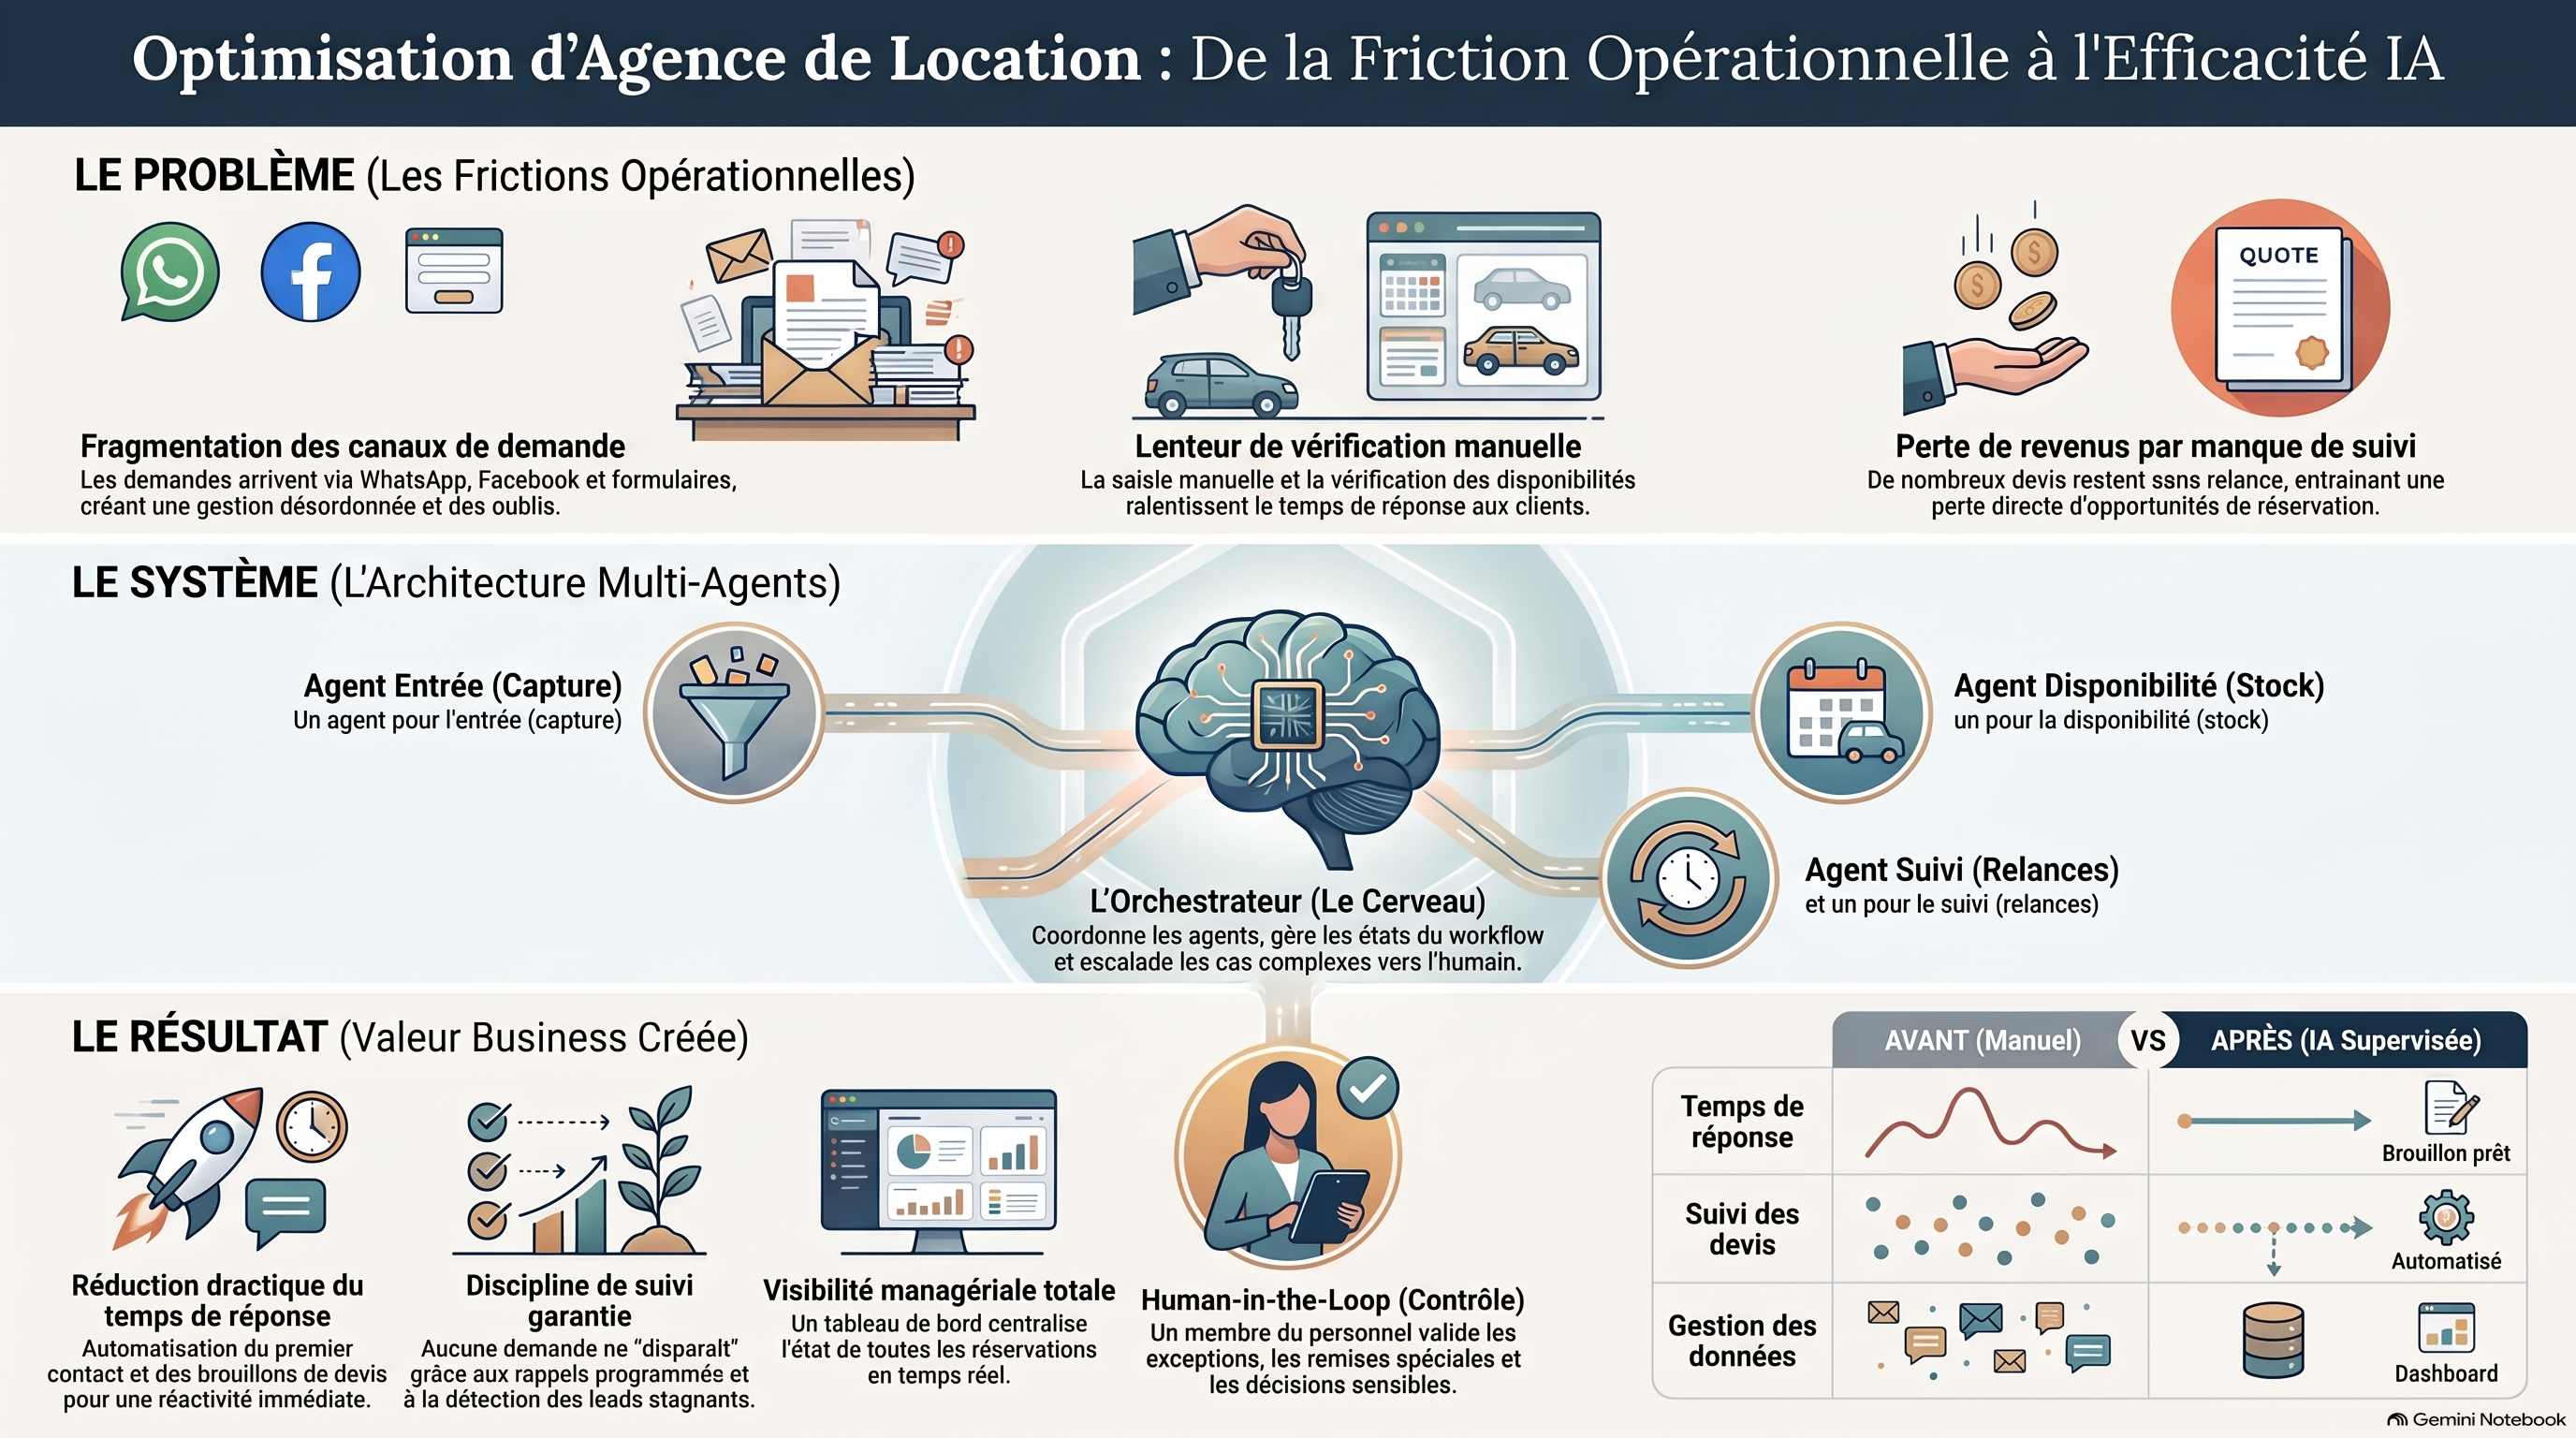
\includegraphics[width=0.95\linewidth]{fig_infographie_probleme_solution.png}
\caption{Infographie de synthese : du chaos operationnel multi-canal (WhatsApp, Facebook, telephone, comptoir) au workflow supervise AutoFlow. La partie centrale represente l'ossature du systeme, la partie droite le resultat metier attendu (file de validation lisible, brouillons prets, KPI auditables).}
\label{fig:infoproblem}
\end{figure}

\vspace{0.3cm}

\section{Observation d'une journee-type}

L'audit d'observation, mene sur site pendant deux journees, a permis de reconstruire la sequence typique d'une matinee operationnelle. Cette narration, qui n'a pas vocation a etre exhaustive, illustre le probleme mieux qu'une liste theorique :

\begin{infobox}[Une matinee dans l'agence --- reconstruction narrative]
\itshape Une demande arrive sur WhatsApp pendant qu'un client est au comptoir ; un collegue note les dates sur un carnet ; un autre ouvre le tableur des vehicules ; on verifie si le SUV est revenu de maintenance ; un devis part par retour de message ; le client ne repond pas ; personne n'a le temps de relancer ; trois jours plus tard il a loue ailleurs ; le gerant demande << on en est ou ? >> et la reponse depend de la memoire de chacun.
\end{infobox}

Cette scene, banale, condense les six frictions structurantes que la section suivante formalise. Elle montre egalement que le probleme n'est \emph{pas} la vitesse individuelle des employes --- qui sont competents et efficaces --- mais la \textbf{coordination} et la \textbf{tracabilite} qui manquent des que plusieurs canaux, plusieurs demandes et plusieurs collaborateurs s'entrelacent.

\section{Les six frictions operationnelles}

L'analyse de l'audit permet de synthetiser six frictions structurantes, notees F1 a F6. Ces frictions sont presentees comme des \emph{hypotheses a valider}, jamais comme des faits definitifs : la grille d'audit du kit de prospection permet ulterieurement de les quantifier avec l'agence.

\begin{table}[H]\centering\small
\caption{Les six frictions operationnelles (hypotheses a valider en audit).}
\label{tab:frictions}
\rowcolors{2}{softBlue}{white}
\begin{tabularx}{\textwidth}{c l X}\toprule
\rowcolor{boxBlue!30}\textbf{\#} & \textbf{Friction observee} & \textbf{Cout probable}\\\midrule
F1 & Demandes dispersees sur plusieurs canaux            & Re-saisie, informations incompletes, oublis silencieux\\
F2 & Disponibilite verifiee a la main dans un tableau    & Reponses lentes, risque de double reservation, indisponibilites manquees\\
F3 & Questions repetitives (prix, caution, kilometrage, livraison) & Attention de l'equipe consommee sur du << bruit >>\\
F4 & Relances oubliees apres devis                        & Devis perdus sans que personne ne le voie\\
F5 & Statut des demandes flou (\emph{qui gere ? ou en est-on ?}) & Coordination par messages et memoire, doublons\\
F6 & Visibilite du gerant limitee                         & Pilotage a l'instinct, pas de mesure objective\\
\bottomrule
\end{tabularx}
\end{table}

Ces frictions n'apparaissent dans \emph{aucun bilan comptable}. Elles se paient en minutes perdues, en charge mentale et en clients silencieux --- trois metriques dont la mesure requiert justement l'outil que ce stage vise a produire.

\section{Problematique}

\begin{problembox}[Problematique centrale du stage]
Comment automatiser le traitement des demandes clients d'une PME de services \textbf{sans retirer la decision aux humains ni inventer d'information}, et comment \emph{prouver} --- a un jury academique comme a un gerant non technique --- que le systeme resultant est \textbf{fiable, explicable et mesurable} ?
\end{problembox}

Cette formulation cristallise trois exigences simultanees qui, prises ensemble, excluent plusieurs approches populaires :
\begin{enumerate}[leftmargin=1.5cm]
    \item \emph{Sans retirer la decision aux humains} exclut les agents autonomes qui envoient, remboursent ou refusent sans validation.
    \item \emph{Sans inventer d'information} exclut les extractions LLM non ancrees et les generations de disponibilite hallucinees.
    \item \emph{Prouver au jury et au gerant} exclut les architectures ``boite noire'' inexplicables.
\end{enumerate}

\section{Objectifs du stage}

\subsection{Objectif pedagogique}
Le projet vise a maitriser la chaine complete d'un \emph{AI Engineer} moderne : conception d'architecture multi-agents, orchestration de workflows persistants (LangGraph avec \texttt{interrupt} / \texttt{Command}), ingenierie de prompts structures (\emph{structured output}, \emph{evidence gate}, calibration de confiance), API REST (FastAPI, Pydantic), interface d'operateur (React + TypeScript), tests d'integration (pytest), evaluation (metriques, calibration), deploiement conteneurise (Docker, Vercel/Render). Il exige egalement le developpement de competences transverses : communication metier a un dirigeant non technique, kit de prospection commerciale, conformite reglementaire (loi 09-08 marocaine).

\subsection{Objectif technique}
Livrer un prototype V1 demontrable :
\begin{itemize}[leftmargin=1.5cm]
    \item \textbf{Backend} FastAPI exposant $\geq$ 20 routes, orchestrateur LangGraph a 7 noeuds, 3 agents Python, persistance SQLite $\rightarrow$ PostgreSQL, checkpointer.
    \item \textbf{Frontend} React 19 + Vite + TypeScript, 10 ecrans admin, formulaire client public.
    \item \textbf{Donnees} : generateur d'agence realiste, 6 semaines d'historique rejouees a travers le vrai graphe.
    \item \textbf{Tests} : $\geq$ 15 tests d'integration verts, 7 simulations metier jouables.
    \item \textbf{Deploiement} : Docker Compose local, deployable sur Vercel + Render / Railway / Fly, ou tout-Vercel serverless.
\end{itemize}

\subsection{Objectif fonctionnel}
Ameliorer, pour l'agence d'accueil, la \textbf{lisibilite} de sa file de demandes (savoir a tout instant qui gere quoi, dans quel etat, pourquoi), la \textbf{securite} de ses reponses client (aucune information inventee, aucun envoi automatique) et la \textbf{mesurabilite} de sa performance (KPI calculables depuis un journal, comparaison avant/apres pilote). L'objectif n'est \emph{pas} de reduire la charge de travail commerciale --- c'est un effet possible a mesurer en pilote --- mais d'\textbf{organiser} l'existant.

\section{Organisation du rapport}

Le manuscrit se deroule en sept chapitres logiquement enchaines. Le present chapitre pose le contexte. Le \textbf{chapitre~2} presente l'etat de l'art des systemes multi-agents et des cadres d'orchestration en septembre 2026, et justifie les choix techniques par des \emph{decision records}. Le \textbf{chapitre~3} formalise le cahier des charges (acteurs, exigences fonctionnelles et non fonctionnelles, perimetre, contraintes). Le \textbf{chapitre~4} detaille la conception architecturale selon la methodologie C4 en sept vues, la machine a dix etats et la matrice d'escalade. Le \textbf{chapitre~5} decrit la realisation des trois agents et de l'orchestrateur LangGraph, avec extraits de code commentes. Le \textbf{chapitre~6} presente l'API FastAPI, l'espace d'administration React et les integrations n8n. Le \textbf{chapitre~7} rend compte de l'evaluation quantitative (16 tests, exactitude, calibration, robustesse) et cadre la mesure des indicateurs metier. Une conclusion generale, une bibliographie et des annexes cloturent le rapport.

\section{Conclusion}

Ce chapitre a pose le contexte metier et formule la problematique centrale du stage. L'agence de location de voitures de Rabat presente un cas d'usage representatif des PME de services marocaines : multi-canalité, multilinguisme informel, sensibilite au prix, absence d'outillage integre. Les six frictions F1--F6 identifiees en audit motivent une intervention ciblee, dont la valeur reside moins dans la reduction d'effectif que dans la mise en ordre de la coordination et la production d'une visibilite auditable. Le chapitre suivant examine l'etat de l'art des solutions techniques susceptibles de repondre a cette problematique et justifie les choix retenus par des \emph{decision records} explicites.

% ================================================================
\chapter{Etat de l'Art et Choix Techniques}\label{chap:etat_art}
% ================================================================
Ce chapitre positionne AutoFlow dans le paysage technologique de septembre 2026. Il passe en revue les approches classiques d'automatisation (RPA, low-code) et leurs limites face au langage naturel, presente les cadres d'orchestration d'agents fondes sur les LLM (LangGraph, Microsoft Agent Framework, CrewAI, AutoGen), analyse les techniques d'extraction d'information structuree \emph{gardees par la preuve}, discute la place de l'humain dans la boucle (\emph{human-in-the-loop}) et conclut par un tableau de decisions techniques explicites.

\section{Introduction}
Un projet d'IA en 2026 se construit rarement \emph{ex nihilo} : il assemble des briques open source matures dont il faut connaitre les forces, les faiblesses et les tendances d'adoption. Ce chapitre etablit la cartographie technique dans laquelle AutoFlow s'inscrit, puis justifie chaque choix majeur par un \emph{decision record} qui explicite le contexte, l'option retenue, les alternatives ecartees et le cout de retour arriere.

\section{Automatisation classique : RPA et plateformes low-code}

Les plateformes d'\textbf{automatisation robotisee des processus (RPA)} --- UiPath, Automation Anywhere, Blue Prism --- et les plateformes \textbf{low-code} --- n8n, Make, Zapier, Power Automate --- constituent la premiere generation d'outils d'automatisation d'entreprise. Elles excellent dans un scenario bien defini : \emph{relier des applications, transformer des payloads structures, declencher des actions sur des evenements calendaires ou webhooks}. Un devis Salesforce declenche l'envoi d'un email Mailchimp, une commande Shopify cree une ligne dans Google Sheets, un formulaire Typeform poste dans Slack : ces cas sont resolus en minutes.

Leur limite apparait des que \textbf{l'entree est du langage naturel} et que l'\textbf{etat metier} doit etre tenu et raisonne. n8n ne comprend pas << je voudrais un SUV a partir du week-end prochain, avec livraison a l'aeroport si possible >> : il faut lui donner des champs deja extraits. Il ne sait pas non plus qu'une demande << attend le client depuis 48h et il faut la relancer >> : il faut lui construire un cron. Ces plateformes restent donc precieuses en \textbf{peripherie} d'un systeme, comme colle vers les canaux et couche de notifications, mais elles ne peuvent pas etre le \textbf{coeur de decision} d'un workflow qui traite du langage.

\section{Agents LLM et cadres d'orchestration}

\subsection{L'emergence des cadres orientes graphes d'etats}
Depuis 2024, une convergence architecturale s'est produite : les cadres d'orchestration d'agents ont abandonne le paradigme du << LLM libre equipe d'outils >> pour adopter des \textbf{graphes d'etats persistants}. La motivation est double : besoin de \emph{reprise apres arret} (checkpointing), et besoin de \emph{validation humaine} sur les decisions a enjeu.

\subsection{LangGraph (LangChain)}
\textbf{LangGraph} modelise un workflow comme un graphe dont les noeuds sont des fonctions Python et les aretes sont des decisions conditionnelles. Il offre le \textbf{checkpointing} (persistance par \texttt{SqliteSaver}, \texttt{PostgresSaver}, etc.), l'\textbf{interruption} pour validation humaine (\texttt{interrupt(payload)}) et la reprise par commande (\texttt{Command(resume=decision)} ou \texttt{Command(goto=noeud)}). Le choix est justifie ici par ces proprietes verifiables dans le code --- persistance, suspension, reprise et visualisation du graphe --- plutot que par des compteurs publics instables. Sa documentation et son integration a l'ecosysteme LangChain (\texttt{init\_chat\_model}, \texttt{with\_structured\_output}) en font un choix adapte a un prototype supervise.

\subsection{Microsoft Agent Framework}
Le \textbf{Microsoft Agent Framework} (2025--2026) propose des graphes de workflows, l'observabilite integree (OpenTelemetry, Azure Monitor) et le checkpointing en Python, .NET et Go. Il est particulierement attractif pour les organisations deja engagees dans l'ecosysteme Azure. Sa courbe d'adoption est prometteuse (13,6~k etoiles en un an), mais son integration a l'infrastructure Azure --- Key Vault, Service Bus, Cosmos DB --- consommerait le budget-temps d'un pilote de PME sans apporter de valeur incrementale. Il est retenu comme candidat serieux pour une \emph{version entreprise ulterieure}, hors perimetre du present stage.

\subsection{CrewAI et AutoGen}
Les cadres \textbf{CrewAI} et \textbf{AutoGen} privilegient la \emph{conversation entre agents} : plusieurs LLM se parlent pour resoudre une tache. Ce paradigme excelle pour des taches ouvertes de recherche ou de creation collective, mais s'accommode mal d'une \textbf{machine a etats explicite} avec transitions legales, ce qui est justement la contrainte imposee par la matrice d'escalade d'AutoFlow.

\subsection{Standards emergents : MCP et A2A}
Deux standards emergent en 2025--2026 : \textbf{MCP (Model Context Protocol)}, propose par Anthropic, qui standardise l'exposition d'outils aux modeles LLM ; et \textbf{A2A (Agent-to-Agent)}, qui specifie la communication entre agents autonomes. AutoFlow reste en \textbf{veille} sur ces standards : MCP deviendra pertinent si un LLM avec outils est retenu apres le pilote ; A2A est inutile a un seul orchestrateur.

\begin{table}[H]\centering\small
\caption{Comparaison des cadres d'orchestration multi-agents (septembre 2026).}
\label{tab:frameworks}
\rowcolors{2}{softBlue}{white}
\begin{tabularx}{\textwidth}{l X X X}\toprule
\rowcolor{boxBlue!30}\textbf{Critere} & \textbf{LangGraph} & \textbf{MS Agent Framework} & \textbf{CrewAI / AutoGen}\\\midrule
Paradigme      & Graphe d'etats + noeuds & Graphe de workflows + observabilite & Conversation multi-agents\\
HITL natif     & \checkmark (\texttt{interrupt}) & \checkmark & Partiel\\
Checkpointing  & \checkmark (SqliteSaver, PostgresSaver) & \checkmark & Non\\
Adoption 2026  & $\sim$42k etoiles         & $\sim$13,6k etoiles & Communautaire\\
Dependance cloud & Aucune               & Azure                & Aucune\\
Cout d'entree PME & Faible              & Eleve (infra Azure)  & Faible\\
\bottomrule
\end{tabularx}
\end{table}

\section{Extraction d'information structuree et confiance}

\subsection{Le probleme de l'hallucination}
Les LLM produisent des sorties structurees fiables lorsqu'un schema est impose (\emph{structured output} via \texttt{with\_structured\_output}, JSON Schema, fonction calling), mais restent \textbf{intrinsequement sujets a l'hallucination} : ils peuvent generer une date qui n'est pas dans le message source, une categorie de vehicule non demandee, un lieu invente. Cette propriete rend l'extraction LLM \emph{non deployable seule} dans un contexte commercial ou l'agent commercial engage la parole de l'entreprise.

\subsection{L'ancrage par la preuve (\emph{evidence gate})}
Deux garde-fous ont ete retenus. Le premier est l'\textbf{ancrage par la preuve} : chaque champ produit par le LLM doit citer un passage \emph{exactement present} dans le texte source. Techniquement, apres extraction, on verifie que le champ \texttt{evidence[k]} est une sous-chaine de la variante normalisee du message ; sinon, le champ est \textbf{rejete} (valeur \texttt{null}, confiance $= 0$). Ce mecanisme rend l'hallucination \emph{structurellement impossible pour les champs}.

\subsection{La calibration de la confiance}
Le second est la \textbf{calibration} : un score de confiance n'a de valeur que s'il predit reellement la justesse. La calibration se mesure : sur les extractions ayant re\c cu une confiance $\geq 0{,}8$, quelle proportion est effectivement correcte ? AutoFlow expose \texttt{field\_confidence[k]} par champ et une \texttt{confidence} globale, comparees a des seuils versionnes dans \texttt{rules.json}. La section 7.4 confirme empiriquement que le seuil est bien place.

\subsection{Inspiration : Jev AI --- << probabilites, pas prose >>}
L'approche de \emph{Jev AI (TypeSafe)} --- << des decisions typees avec une probabilite calibree, pas de la prose >> --- inspire la representation des sorties de l'agent Intake sous forme de \texttt{signals} numeriques : \texttt{is\_complaint: 0.92}, \texttt{discount\_requested: 0.85}, \texttt{dates\_ambiguous: 0.55}. L'orchestrateur ne lit \emph{jamais} du texte libre : il compare des nombres a des seuils. Cette discipline supprime la principale source de fragilite des orchestrateurs << conversationnels >> : la sensibilite au phrasing des sorties LLM.

\section{Human-in-the-loop : de la contrainte a la feature}

La litterature sur l'automatisation sure converge : les decisions a enjeu --- argent, identite, emotion --- doivent rester humaines. L'ecole de \emph{safe AI} formalise ce principe sous le nom de \textbf{human-in-the-loop (HITL)} : l'humain n'est pas un repli de l'IA faible, mais un \textbf{point de controle structurel} qui garantit la responsabilite juridique et commerciale.

Dans AutoFlow, HITL n'est pas un \emph{fallback} d'exception : c'est une \textbf{feature centrale}. Chaque demande passe par un \texttt{interrupt()} au moins une fois avant d'atteindre le client. Le payload d'interruption --- persiste par le checkpointer LangGraph --- contient la raison de la revue, le niveau requis (equipe ou manager), le brouillon prepare et les actions autorisees. L'humain \emph{approuve}, \emph{modifie}, \emph{refuse}, \emph{complete} ou \emph{clot} ; l'orchestrateur reprend via \texttt{Command(resume=\dots)} ou \texttt{Command(goto=availability)}.

\begin{mechanismbox}[Le contrat de fiabilite d'AutoFlow]
Trois invariants non negociables :
\begin{enumerate}
\item Le systeme \textbf{n'envoie jamais} un message au client seul (l'envoi est un clic humain).
\item Le systeme \textbf{n'invente jamais} une disponibilite (code deterministe) ni un champ (evidence gate).
\item \textbf{Tout est trace} : chaque transition ecrit un evenement (acteur, raison, horodatage).
\end{enumerate}
Ces trois invariants sont verifiables par relecture de code et par tests d'integration (chapitre~7).
\end{mechanismbox}

\section{Synthese : le stack technique retenu}

\begin{table}[H]\centering\small
\caption{Stack technique d'AutoFlow --- decision records synthetises.}
\label{tab:stack}
\rowcolors{2}{softGreen}{white}
\begin{tabularx}{\textwidth}{l l X}\toprule
\rowcolor{emsiGreen!30}\textbf{Composant} & \textbf{Techno} & \textbf{Justification courte}\\\midrule
Orchestrateur        & LangGraph 1.2                 & HITL + checkpointing natifs, graphe lisible, adoption\\
Backend API          & FastAPI + Pydantic            & Schemas partages avec les agents, OpenAPI gratuit\\
Persistance          & SQLAlchemy 2 + SQLite/Postgres & Laptop en pilote, cloud sans redesign\\
Extraction LLM       & LangChain \texttt{with\_structured\_output} + \emph{evidence gate} & Optionnel, anti-hallucination structurelle\\
Frontend             & React 19 + Vite + TypeScript  & Build statique deployable sur Vercel/Netlify\\
Diagramme workflow   & Mermaid inline (SVG)          & Le graphe et le code ne divergent pas\\
Notifications        & n8n (community)               & 280+ templates, notifie sans envoyer\\
Tests                & pytest + FastAPI TestClient   & 16 tests couvrant les scenarios metier\\
Deploiement          & Docker + Vercel/Render/Fly    & Cout $\approx$ 0~MAD en pilote\\
\bottomrule
\end{tabularx}
\end{table}

\section{Modele economique pour l'agence}

Le stack a ete choisi non seulement pour ses proprietes techniques, mais aussi pour son \textbf{cout d'operation quasi nul}. Un pilote peut tourner sur le laptop du gerant sans installation payante ; une phase distante utilise les offres gratuites de Vercel + Render + Neon. Le LLM est optionnel : en mode \texttt{LLM\_PROVIDER=none}, le moteur de regles suffit a operer, et le cout d'appel LLM (Anthropic Haiku, OpenAI GPT-4o-mini) plafonne a quelques centimes de MAD par demande. Toutes les licences sont libres (MIT/Apache).

Positionnement commercial : \emph{un outil quasi gratuit a faire tourner, facture sur le temps d'audit et d'adaptation, jamais sur une licence}.

\section{Conclusion}

Ce chapitre a etabli que le paysage 2026 privilegie les \textbf{graphes d'etats persistants} sur les agents LLM libres. LangGraph a ete retenu pour sa maturite, son support natif du HITL et son integration a l'ecosysteme LangChain. L'extraction d'information est \emph{gardee par la preuve} et exprimee sous forme de signaux calibres. L'humain dans la boucle est promu au rang de \emph{feature centrale}, non de repli. Le chapitre suivant traduit ces choix en un cahier des charges fonctionnel et non fonctionnel formel.

% ================================================================
\chapter{Analyse des Besoins et Cahier des Charges}\label{chap:besoins}
% ================================================================
Ce chapitre transforme les intentions du chapitre~1 et les choix techniques du chapitre~2 en un cahier des charges verifiable. Il identifie les acteurs du systeme et leurs attentes, formalise les exigences fonctionnelles (RF1--RF10) et non fonctionnelles, precise le perimetre inclus et exclu, expose les contraintes et hypotheses, et etablit la matrice d'alignement avec les objectifs pedagogiques du stage.

\section{Introduction}
Un cahier des charges bien redige n'est pas une liste de vux, c'est un \emph{contrat verifiable}. Chaque exigence de ce chapitre est associee a un moyen de verification --- test automatise, code source, mesure --- de sorte que la conformite du prototype puisse etre objectivement etablie au chapitre~7.

\section{Identification des acteurs}

L'analyse fonctionnelle fait emerger quatre acteurs dont les perimetres d'action et les attentes sont distincts. Le tableau~\ref{tab:acteurs} les synthetise.

\begin{table}[H]\centering\small
\caption{Acteurs du systeme AutoFlow et leurs attentes prioritaires.}
\label{tab:acteurs}
\rowcolors{2}{softPurple}{white}
\begin{tabularx}{\textwidth}{l X X}\toprule
\rowcolor{layerPres!30}\textbf{Acteur} & \textbf{Role dans le workflow} & \textbf{Besoins prioritaires}\\\midrule
Client              & Emetteur des demandes, en langage naturel & Reponse rapide, precise, propositions d'alternatives\\
Equipe commerciale  & Validation, envoi, modification des brouillons, saisie des reponses client & File claire, brouillons pertinents, raison lisible\\
Manager             & Decisions sensibles : remises, reclamations, longues durees, valeurs elevees, refus & Vue synthetique, matrice d'escalade explicite, tracabilite\\
Systeme             & Structure, verifie, prepare, route, journalise, rappelle & Regles versionnees, invariants respectes, aucun envoi seul\\
\bottomrule
\end{tabularx}
\end{table}

Le \textbf{client} n'interagit \emph{jamais} directement avec le systeme : il ecrit sur WhatsApp, Facebook ou remplit un formulaire ; c'est l'equipe qui manipule l'interface. Cette separation garantit que la relation commerciale reste humaine, meme si sa preparation est assistee.

\section{Exigences fonctionnelles (RF1--RF10)}

\begin{table}[H]\centering\small
\caption{Exigences fonctionnelles et moyens de verification associes.}
\label{tab:rf}
\rowcolors{2}{softBlue}{white}
\begin{tabularx}{\textwidth}{l X l}\toprule
\rowcolor{boxBlue!30}\textbf{ID} & \textbf{Exigence} & \textbf{Verification}\\\midrule
RF1  & Toute demande recue obtient un identifiant, un etat initial et un evenement journalisation & \texttt{test\_scenario\_a\_standard\_quote}\\
RF2  & Le systeme ne declare jamais un vehicule disponible sans verification deterministe & \texttt{availability.py}, \texttt{test\_scenario\_b}\\
RF3  & Un champ extrait par LLM sans preuve verbatim est rejete (\emph{evidence gate}) & \texttt{extract\_llm} + \texttt{test\_llm\_gate}\\
RF4  & Toute reclamation est escaladee au manager sans brouillon automatique & \texttt{test\_scenario\_d\_complaint}\\
RF5  & Remise demandee, location $>$14 j, valeur $>$6000 MAD $\rightarrow$ manager & \texttt{decide\_after\_availability}\\
RF6  & Aucun message n'est envoye sans clic humain & \texttt{finalize\_node} uniquement via \texttt{Command(resume)}\\
RF7  & Une relance est planifiee a l'envoi ; au-dela de la politique, \emph{stalled} $\rightarrow$ humain & \texttt{test\_follow\_up\_engine}\\
RF8  & Chaque transition est journalisee avec acteur, raison, horodatage & \texttt{store.transition}\\
RF9  & Les KPI sont calcules depuis le journal, jamais stockes & \texttt{orchestrator.kpis}\\
RF10 & L'espace admin exige un token ; le formulaire public n'en exige pas & \texttt{test\_auth\_required}\\
\bottomrule
\end{tabularx}
\end{table}

Ces dix exigences couvrent l'integralite du perimetre V1. Chacune est \textbf{tracee a un moyen de verification} : test automatise, module de code, ou combinaison des deux. La matrice de couverture est presentee au chapitre~7.

\section{Exigences non fonctionnelles}

\begin{table}[H]\centering\small
\caption{Exigences non fonctionnelles et metriques cibles.}
\label{tab:nfr}
\rowcolors{2}{softOrange}{white}
\begin{tabularx}{\textwidth}{>{\bfseries}l X X}\toprule
\rowcolor{boxOrange!30}Critere & Exigence & Metrique cible\\\midrule
Autonomie      & Fonctionnement hors ligne complet (\texttt{LLM\_PROVIDER=none}) & La demo ne depend d'aucune API externe\\
Explicabilite  & Chaque routage doit etre justifiable par une regle et une valeur mesuree & Panneau \emph{Suivi en direct} avec chemin allume\\
Reprise        & L'etat du workflow survit a un redemarrage & Checkpointer SQLite, \texttt{pending\_interrupt} conserve\\
Confidentialite & Telephones masques, donnees fictives ; seul le texte du message vers un LLM (si active) & Conforme au principe de minimisation\\
Reglementation & Loi 09-08 (protection des donnees personnelles au Maroc) & A cadrer avec l'agence avant tout usage de donnees reelles\\
Simplicite     & Code metier concis, lisible en journee & $<$ 1500 lignes de Python metier\\
Deployabilite  & Deployable sur laptop, cloud gere ou serverless & Docker Compose, Vercel/Render, Vercel Python\\
Cout           & Infrastructure quasi nulle pour l'agence & $\approx$~0 MAD en pilote local, $\sim$5--7~\$/mois cloud\\
\bottomrule
\end{tabularx}
\end{table}

\section{Perimetre inclus et exclu}

\subsection{Fonctionnalites incluses (V1 demontrable)}
Le perimetre V1 comprend : saisie manuelle et formulaire public \texttt{/demande} et webhook n8n ; les trois agents (Intake, Disponibilite, Suivi) ; l'orchestrateur LangGraph ; l'espace d'administration en dix ecrans (tableau de bord, file a valider, suivi en direct, simulations, demandes, fiche demande, nouvelle demande, flotte \& regles, architecture, mode presentation) ; le jeu de donnees realiste (24 vehicules, 80 reservations, 40 clients, 45 demandes sur 6 semaines rejouees) ; les sept simulations metier jouables ; le deploiement Vercel/Netlify + Docker ou Vercel Python.

\subsection{Fonctionnalites exclues (\emph{audit-gated})}
Sont \textbf{explicitement exclues} du perimetre V1 : le paiement en ligne, la tarification dynamique, l'envoi automatique de messages au client, le connecteur WhatsApp Business ou Instagram \emph{en direct} (n8n reste en peripherie), l'integration CRM/ERP, la maintenance predictive, la voix. Chaque exclusion est \emph{audit-gated} : elle n'entre au perimetre que si l'audit sur site prouve son besoin operationnel.

\section{Contraintes et hypotheses}

\begin{itemize}[leftmargin=1.5cm]
\item \textbf{Environnement de developpement} : Windows 11 avec Python 3.12+, Node 20+, PowerShell. La compatibilite Linux/mac est assuree par le \texttt{run.sh} et Docker.
\item \textbf{Donnees d'entrainement} : \emph{aucune donnee reelle client n'est utilisee}. Le pilote fonctionne sur un jeu synthetique realiste genere de facon deterministe.
\item \textbf{Compatibilite navigateur} : Chrome, Firefox et Safari recents (ES2020+).
\item \textbf{Absence de secret dans le frontend} : le token admin est saisi a la connexion et stocke uniquement en \texttt{localStorage}.
\item \textbf{Loi 09-08} : le traitement de donnees personnelles reelles requiert un cadrage formel avec l'agence avant tout deploiement.
\end{itemize}

\section{Alignement avec les objectifs pedagogiques}

\begin{table}[H]\centering\small
\caption{Matrice d'alignement entre objectifs pedagogiques et realisations.}
\label{tab:alignement}
\rowcolors{2}{softGreen}{white}
\begin{tabularx}{\textwidth}{X X >{\centering\arraybackslash}p{2cm}}\toprule
\rowcolor{emsiGreen!30}\textbf{Objectif pedagogique} & \textbf{Realisation dans AutoFlow} & \textbf{Etat}\\\midrule
Orchestration multi-agents         & Orchestrateur LangGraph a 7 noeuds, 3 agents & Realise\\
Human-in-the-loop persistant       & \texttt{interrupt()} + \texttt{Command(resume/goto)} + SqliteSaver & Realise\\
Ingenierie de prompts structures   & Sortie typee + \emph{evidence gate} + signaux calibres & Realise\\
API REST                           & FastAPI, 24 routes, OpenAPI genere & Realise\\
Interface d'operateur              & React 19 + Vite + TypeScript, 10 ecrans & Realise\\
Tests d'integration                & 16 tests pytest verts (8 scenarios + 7 simulations + catalogue) & Realise\\
Evaluation quantitative            & Rapport d'exactitude, calibration, filet de securite & Realise\\
Communication metier               & Kit de prospection complet (11 documents, visuels PDF) & Realise\\
Documentation d'architecture       & 7 vues C4, decision records, 4 diagrammes exportables & Realise\\
\bottomrule
\end{tabularx}
\end{table}

\begin{mechanismbox}[Le cahier des charges est un contrat testable]
Contrairement a un cahier des charges narratif, les 10 exigences fonctionnelles et les 8 exigences non fonctionnelles d'AutoFlow sont \emph{tracees a du code executable}. Le chapitre~7 (Evaluation) exhibera la matrice de couverture qui associe chaque exigence a son test.
\end{mechanismbox}

\section{Conclusion}

Le cahier des charges est formalise, les acteurs identifies, le perimetre precise, les contraintes explicitees. Le contrat V1 tient en dix exigences fonctionnelles et huit exigences non fonctionnelles, chacune verifiable par un moyen precis. Le chapitre suivant traduit ce contrat en une architecture logicielle detaillee, presentee selon la methodologie C4 en sept vues complementaires.

% ================================================================
\chapter{Conception Architecturale}\label{chap:conception}
% ================================================================
Ce chapitre presente la conception architecturale d'AutoFlow selon la methodologie C4 (Context, Containers, Components, Code) enrichie de trois vues complementaires : flux de donnees, sequence et defaillances. Il detaille le graphe d'orchestration LangGraph, la machine a dix etats, la matrice d'escalade et le modele de donnees relationnel. La convention adoptee est stricte : trait plein pour un \emph{FACT} verifie dans le code, trait pointille pour une \emph{HYPOTHESIS} a valider avec l'agence.

\section{Introduction}
L'architecture d'AutoFlow a ete concue selon un principe directeur unique : \textbf{la simplicite d'abord}. Un workflow orchestre avec un orchestrateur, trois agents et six outils metier est plus \emph{credible}, plus \emph{testable} et plus \emph{demontrable} que << cinq agents pour faire moderne >>. Ce chapitre expose successivement les sept vues qui, ensemble, decrivent le systeme sans jamais en surcharger un seul schema.

\section{Vue contexte --- qui parle au systeme ?}

La vue contexte identifie les acteurs humains et les systemes externes qui interagissent avec AutoFlow. La \textbf{frontiere-cle}, verifiee dans le code, est qu'AutoFlow \emph{ne communique jamais directement avec le client} : il produit des brouillons qu'une personne clique pour envoyer.

\begin{figure}[H]\centering
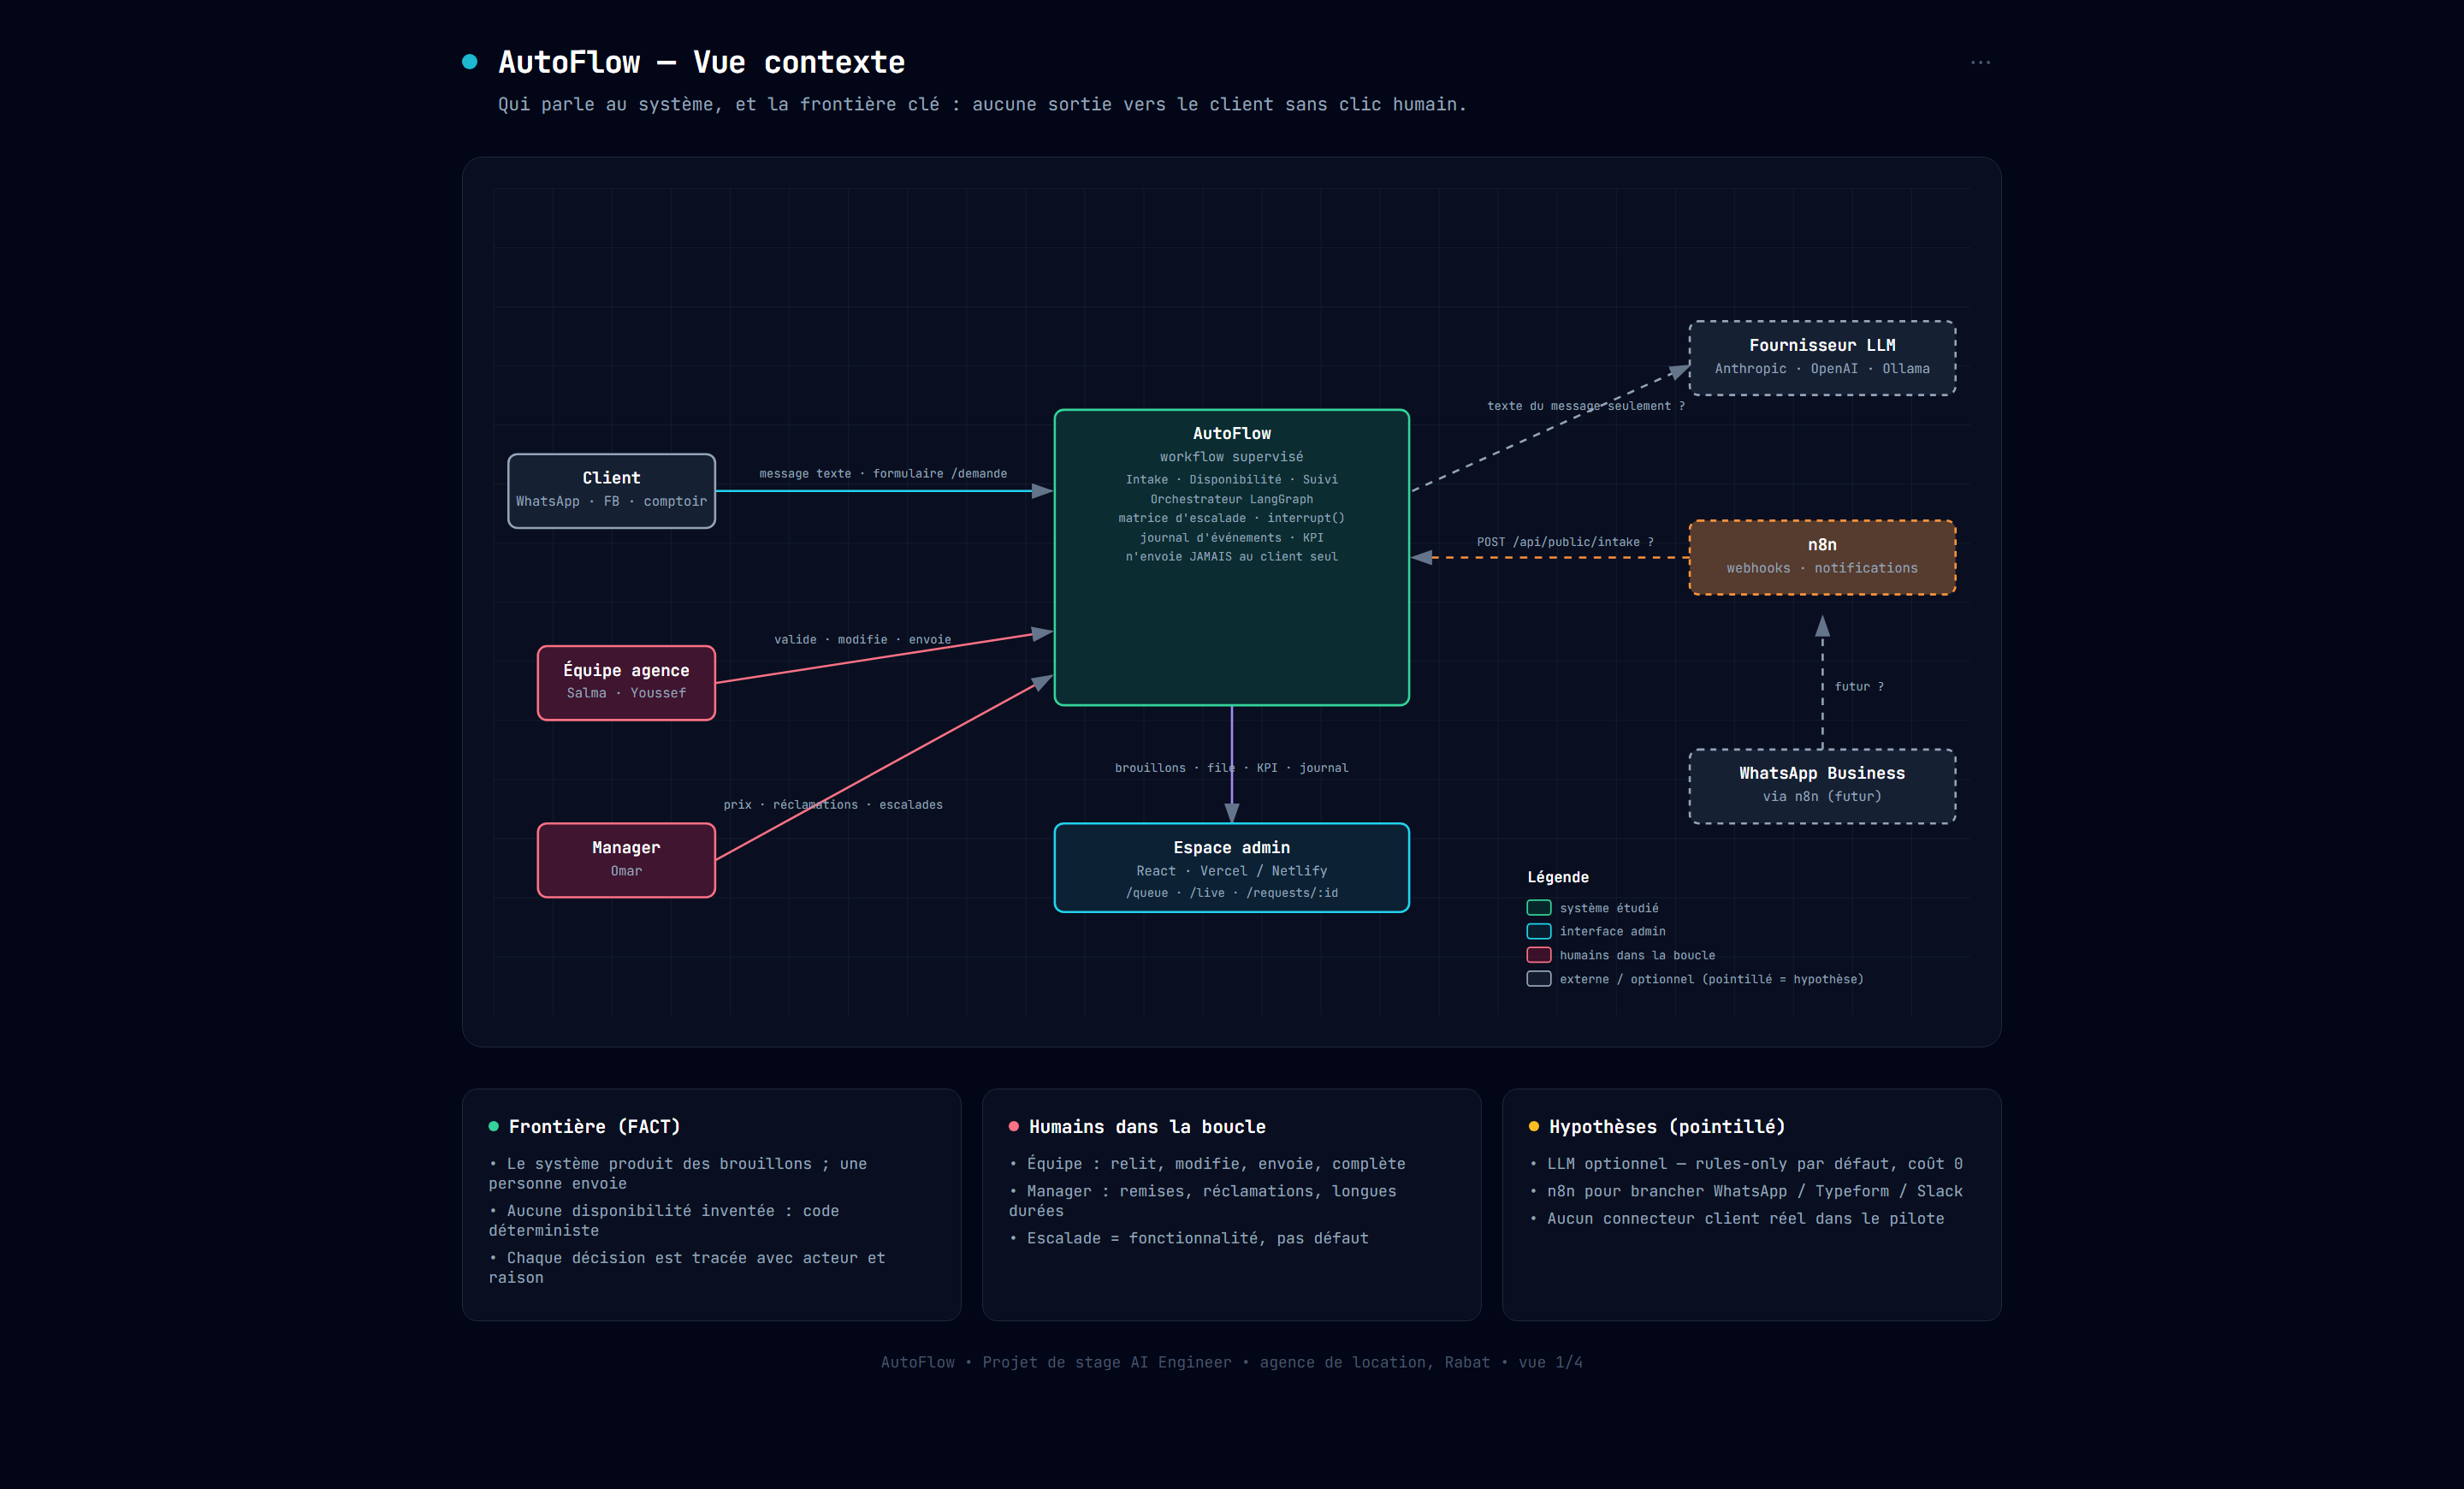
\includegraphics[width=0.95\linewidth]{fig_c4_contexte.png}
\caption{Vue contexte C4. Les acteurs humains (Client, Equipe, Manager) et les systemes externes (LLM optionnel, n8n, WhatsApp Business) sont representes autour du systeme central. Le trait pointille marque les integrations externes non obligatoires.}
\label{fig:c4-contexte}
\end{figure}

\vspace{0.4cm}

\section{Vue conteneurs --- de quoi est fait le systeme ?}

La vue conteneurs decompose AutoFlow en \emph{unites deployables} : un frontend statique React, un backend FastAPI, l'orchestrateur LangGraph, les trois agents, une base relationnelle et un checkpointer. Le frontend est heberge sur Vercel ou Netlify (build statique, aucun secret), le backend sur Docker (Render / Railway / Fly) ou en serverless Vercel Python.

\begin{figure}[H]\centering
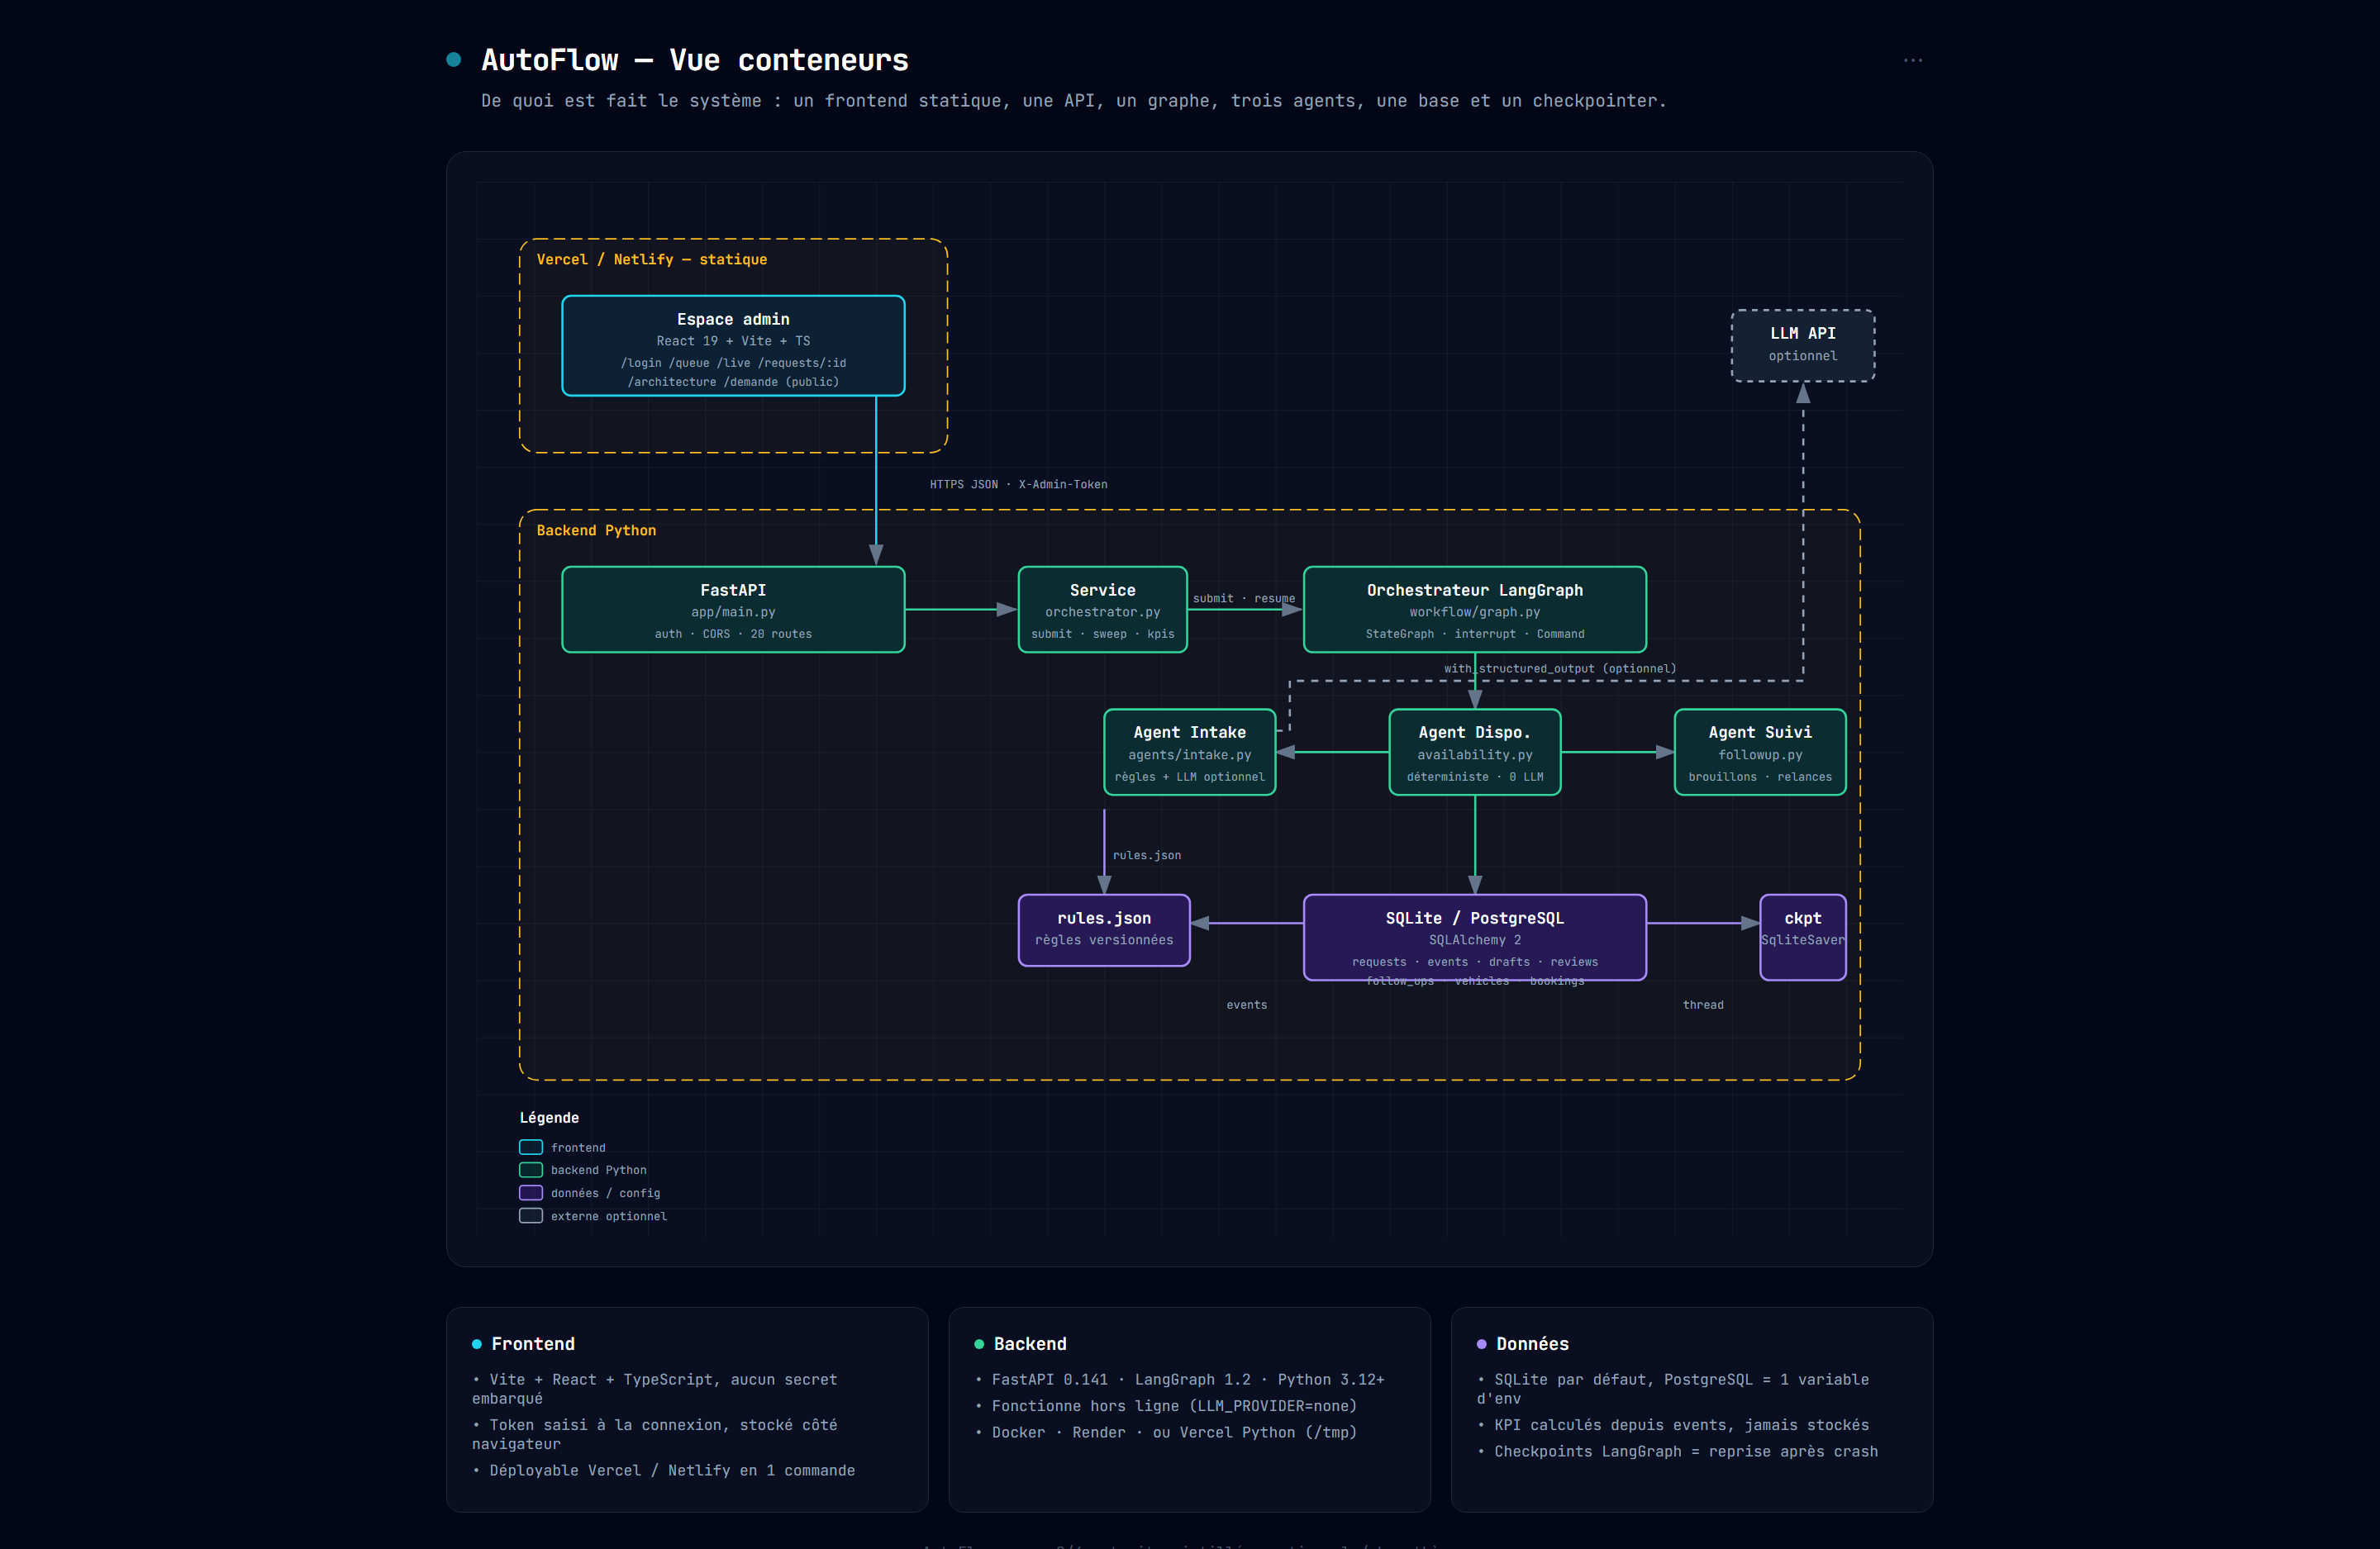
\includegraphics[width=0.95\linewidth]{fig_c4_conteneurs.png}
\caption{Vue conteneurs C4. Le frontend communique avec l'API par HTTPS/JSON. L'orchestrateur pilote les agents et journalise dans SQLite/Postgres. Le checkpointer LangGraph utilise une base dediee pour la reprise apres arret.}
\label{fig:c4-conteneurs}
\end{figure}

\section{Vue composants --- le graphe LangGraph}

Le graphe d'orchestration compte \textbf{sept noeuds} et \textbf{deux gardes conditionnelles}. Le flux nominal est : \texttt{START} $\rightarrow$ \texttt{intake} $\rightarrow$ \texttt{route\_after\_intake} $\rightarrow$ \texttt{\{escalate | clarify | availability\}} $\rightarrow$ \texttt{decide\_after\_availability} $\rightarrow$ \texttt{\{sensitive | draft\}} $\rightarrow$ \texttt{human\_review} (interrupt) $\rightarrow$ \texttt{finalize} $\rightarrow$ \texttt{END}. Le noeud \texttt{human\_review} peut renvoyer vers \texttt{availability} par \texttt{Command(goto=availability)} apres completion des champs manquants par l'humain.

\begin{figure}[H]\centering
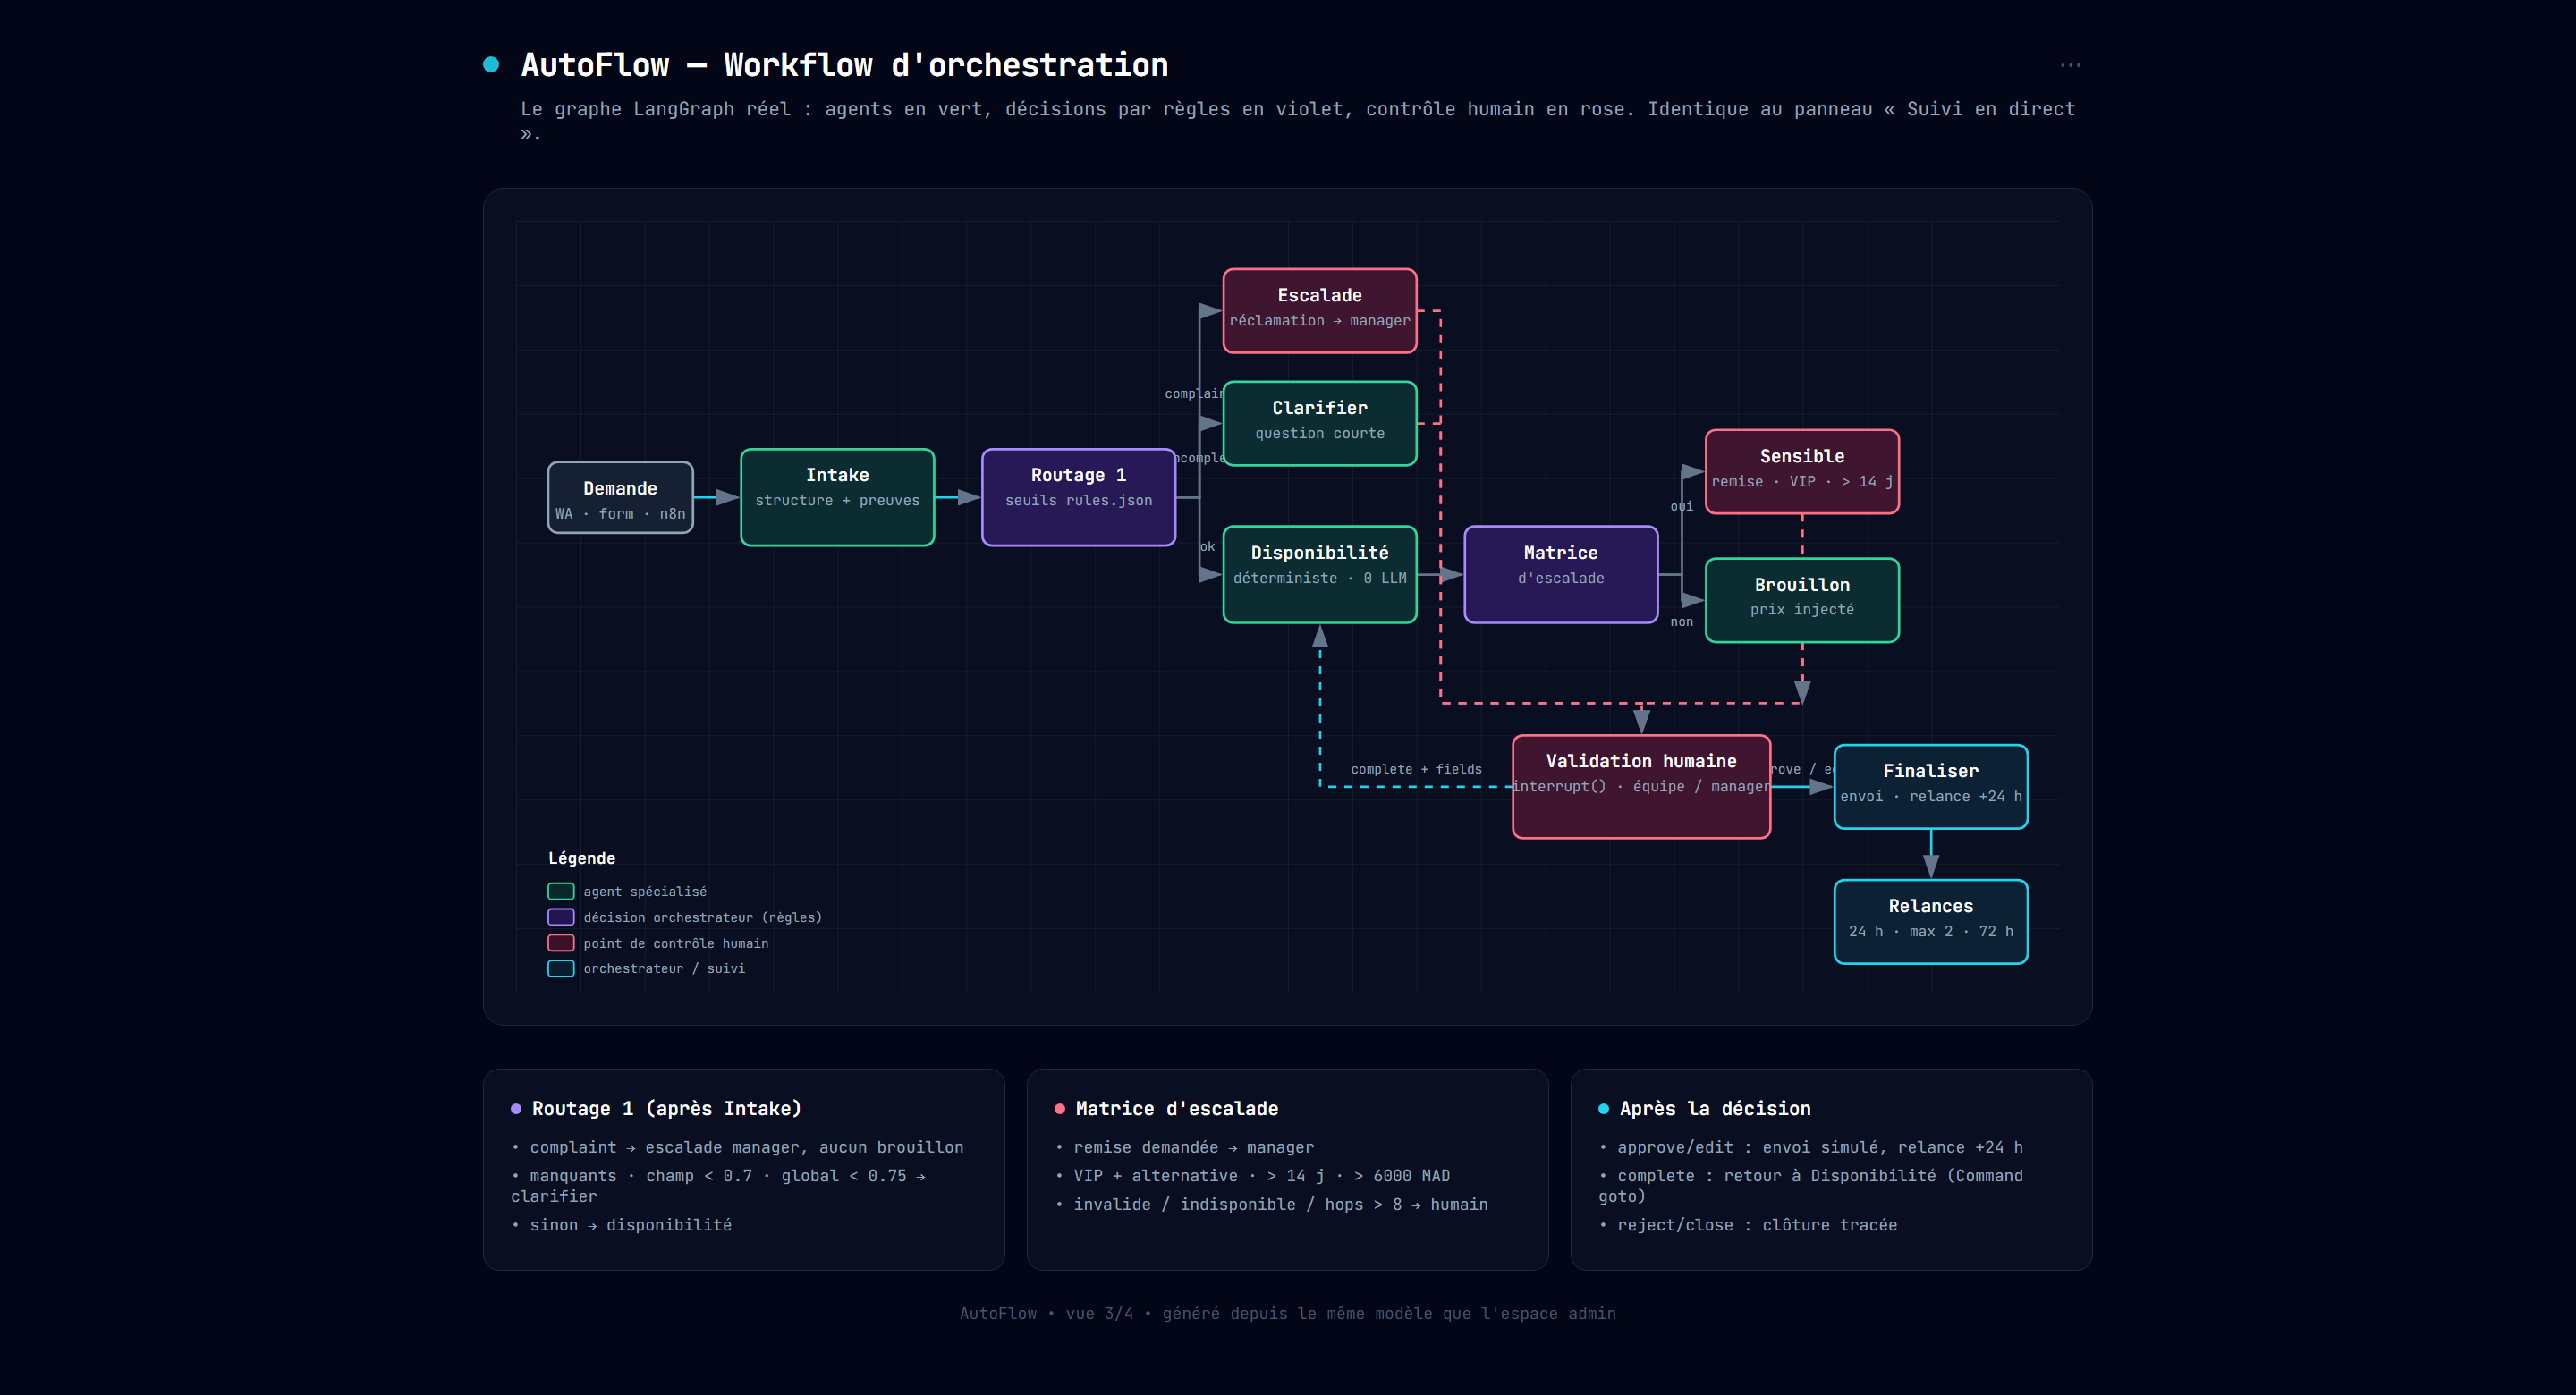
\includegraphics[width=0.95\linewidth]{fig_graphe_langgraph.png}
\caption{Graphe d'orchestration LangGraph. Les losanges representent les gardes conditionnelles (\texttt{route\_after\_intake} et \texttt{decide\_after\_availability}). Le noeud \texttt{human\_review} en style << gate >> materialise le point d'interruption humain. Le graphe est aussi expose par \texttt{GET /api/graph} et affiche dans l'espace admin : le code et le schema \emph{ne peuvent pas diverger}.}
\label{fig:graphe}
\end{figure}

\section{Machine a dix etats et transitions legales}

La machine a etats formalise le cycle de vie d'une demande. Chaque transition passe par \texttt{store.transition()} qui refuse un mouvement illegal (leve \texttt{IllegalTransition}, HTTP 409) et ecrit un evenement dans la table \texttt{events}.

\begin{figure}[H]\centering
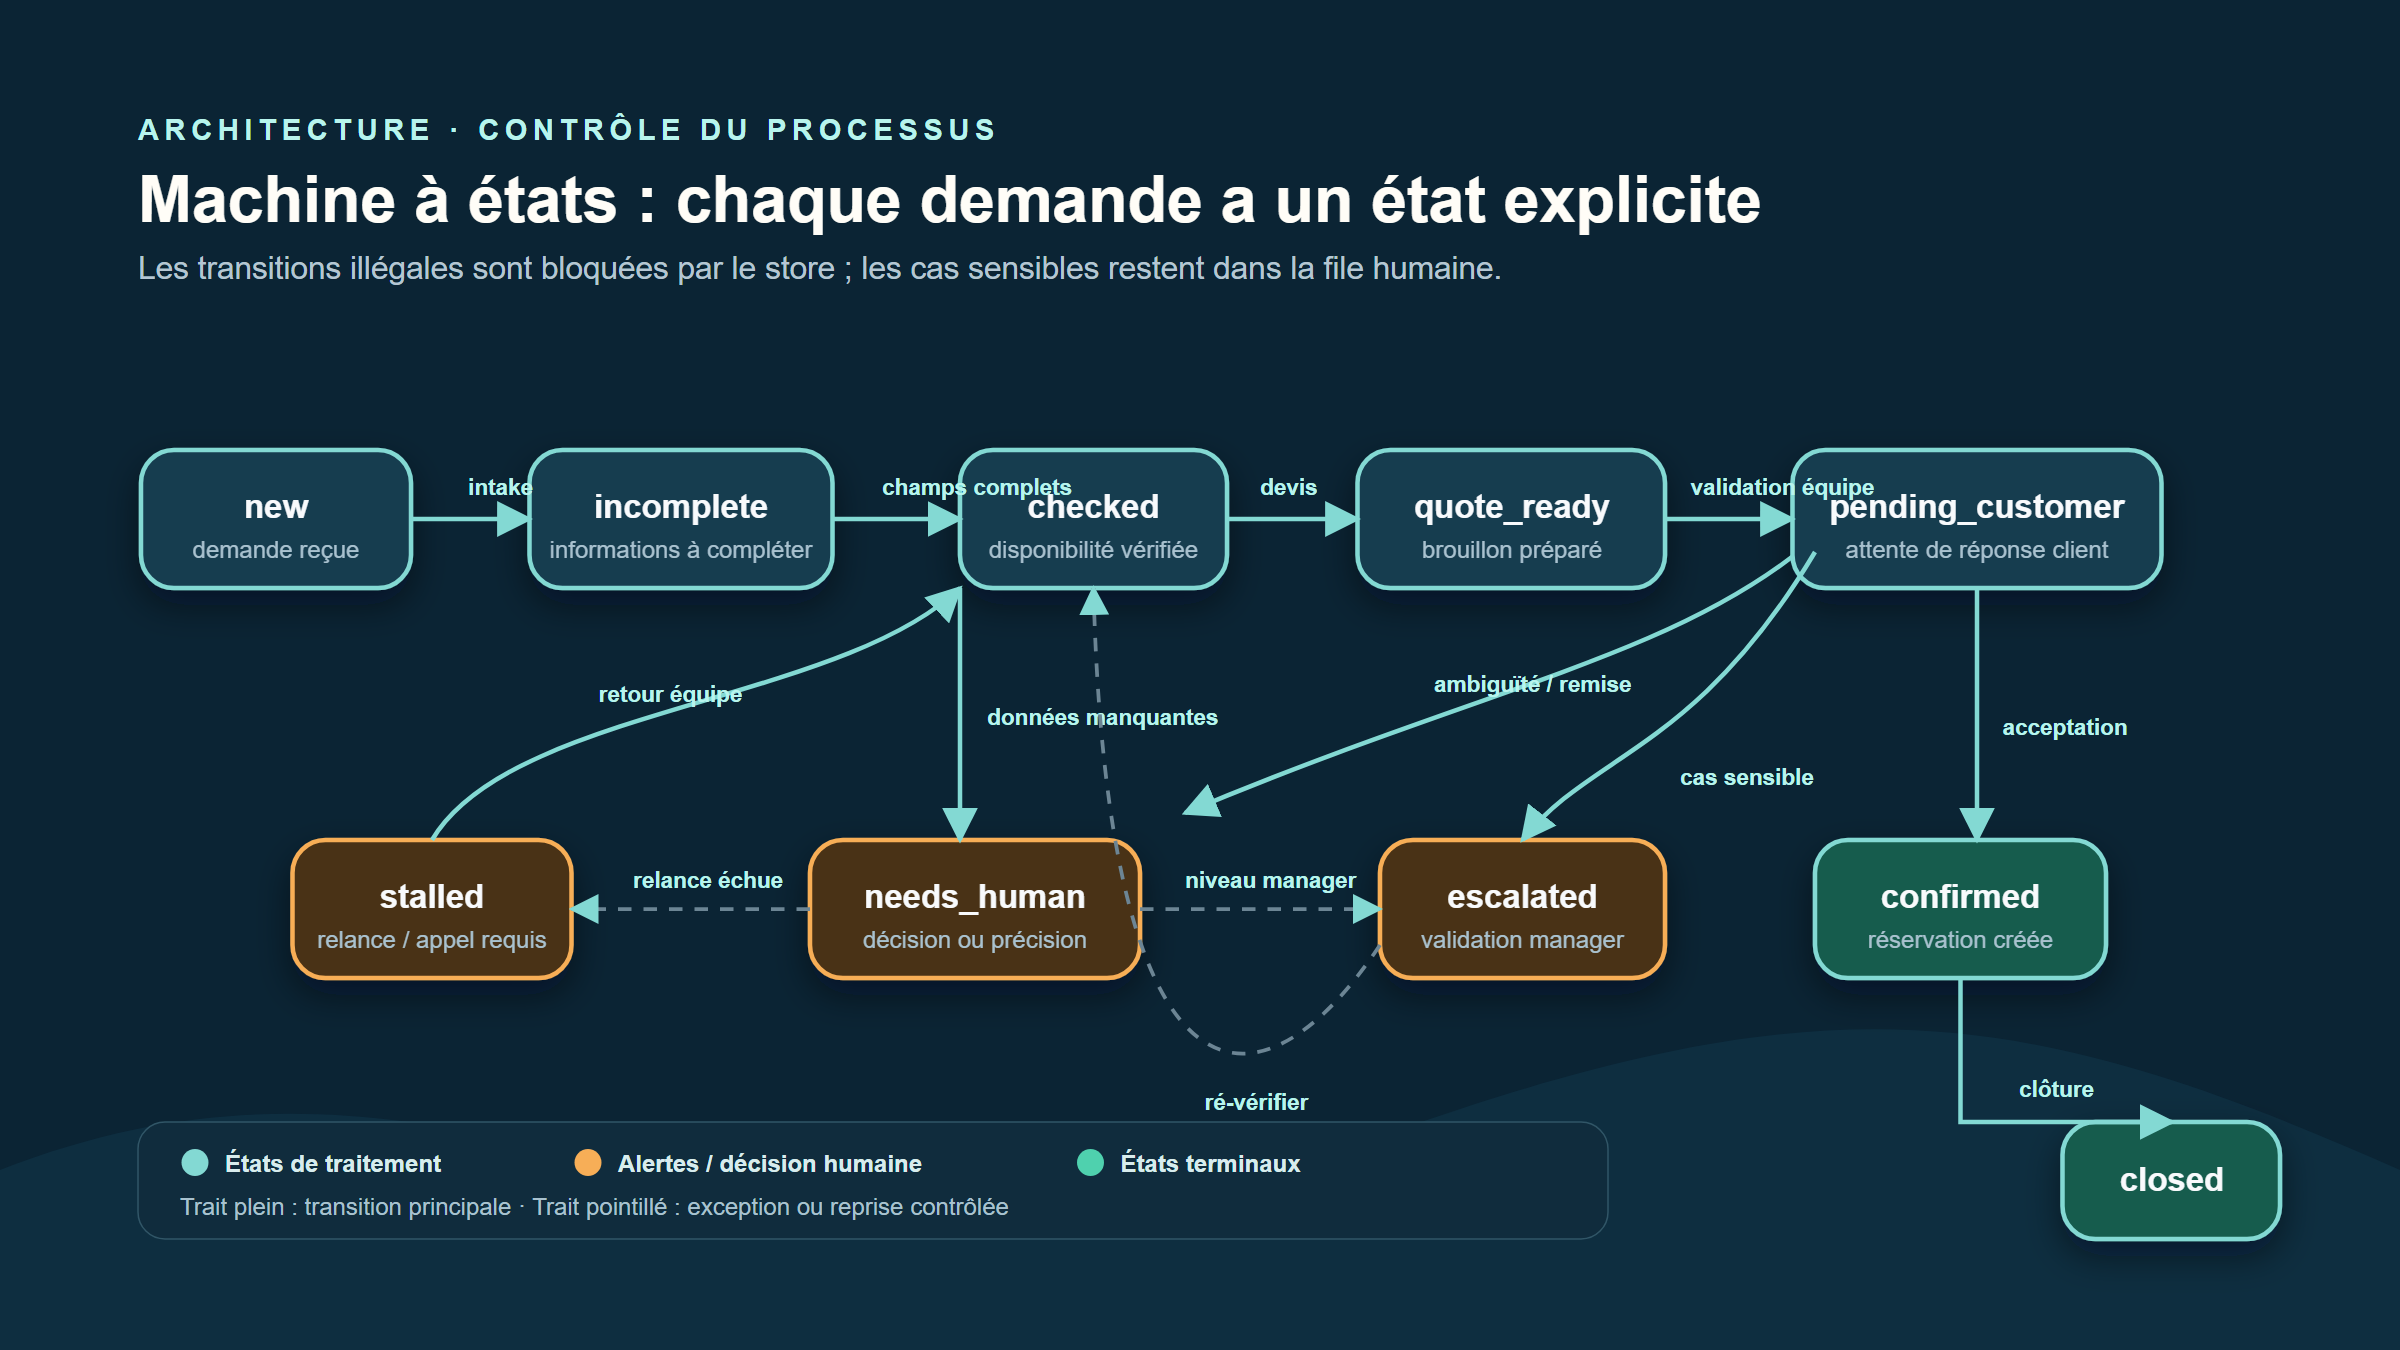
\includegraphics[width=0.9\linewidth]{fig_machine_etats.png}
\caption{Machine a dix etats. Les etats terminaux (\texttt{confirmed}, \texttt{closed}) sont en vert. Les etats d'alerte (\texttt{needs\_human}, \texttt{escalated}, \texttt{stalled}) sont en orange. Les transitions inverses sont possibles depuis \texttt{needs\_human} vers \texttt{checked} (apres completion) et depuis \texttt{pending\_customer} vers \texttt{confirmed} ou \texttt{closed}.}
\label{fig:machine-etats}
\end{figure}

Les dix etats sont : \texttt{new} (demande recue), \texttt{incomplete} (champs manquants), \texttt{checked} (Intake termine), \texttt{quote\_ready} (brouillon pret), \texttt{pending\_customer} (envoye au client, en attente de reponse), \texttt{stalled} (client silencieux depuis 72 h), \texttt{needs\_human} (revue equipe), \texttt{escalated} (revue manager), \texttt{confirmed} (reservation creee), \texttt{closed} (dossier clos).

\section{Matrice d'escalade}

La matrice d'escalade formalise la question centrale : \textbf{qui doit decider quoi, et pourquoi} ? Elle est evaluee par la garde \texttt{decide\_after\_availability} apres verification de la disponibilite.

\begin{table}[H]\centering\small
\caption{Matrice d'escalade appliquee apres verification de disponibilite.}
\label{tab:escalade}
\rowcolors{2}{softBlue}{white}
\begin{tabularx}{\textwidth}{X l l}\toprule
\rowcolor{boxBlue!30}\textbf{Declencheur} & \textbf{Niveau} & \textbf{Etat cible}\\\midrule
Reclamation                                       & Manager & \texttt{escalated}\\
Champs manquants ou confiance globale $<$ 0{,}75  & Equipe  & \texttt{needs\_human}\\
Confiance de champ critique $<$ 0{,}7             & Equipe  & \texttt{needs\_human}\\
Remise demandee                                   & Manager & \texttt{escalated}\\
Client regulier avec alternative proposee         & Equipe  & \texttt{needs\_human}\\
Duree $>$ 14 jours                                & Manager & \texttt{escalated}\\
Valeur $>$ 6000 MAD                               & Manager & \texttt{escalated}\\
Statut invalide ou indisponible                   & Equipe  & \texttt{needs\_human}\\
Plus de 8 sauts (\emph{anti-boucle})              & Equipe  & \texttt{needs\_human}\\
\bottomrule
\end{tabularx}
\end{table}

Cette matrice est \emph{explicite}, \emph{versionnee} (dans \texttt{rules.json}) et \emph{auditable}. C'est elle qui donne au gerant la certitude qu'aucune remise, aucune reclamation, aucune reservation exceptionnelle ne sera prise sans son accord.

\section{Vue flux de donnees}

Le trajet complet d'un message brut a travers le pipeline est le suivant :

\begin{lstlisting}[caption={Trajet d'un message brut a travers le pipeline supervise.}]
Message brut (str, francais / darija)
  -> Intake        : normalisation NFD + regex dates FR + mots-cles
                     + [LLM structured output + preuve verbatim]
  -> StructuredRequest {intent, dates ISO, categorie, boite, lieux,
                        flags[], field_confidence{}, confidence,
                        missing[], evidence{}, signals{}}
  -> Orchestrateur : comparaison signaux vs rules.json -> route
  -> Disponibilite : SELECT vehicles, bookings -> chevauchement
                     + tampon 4 h + maintenance + replis
                     -> AvailabilityResult {status, options[],
                        alternatives[], reasons[]}
  -> Matrice d'escalade -> Review {level, priority, reason}
  -> Suivi         : template FR + injection prix depuis la table
                     -> FollowUpOutput {draft_kind, draft_fr, action}
  -> interrupt()   : payload persiste (checkpoint) ;
                     DB : Request.state, Draft, Review, Event
  -> Decision humaine (JSON) -> Command(resume) -> finalize
                     Draft.sent_at, FollowUp.due_at = now + 24 h
  -> Sweep         : FollowUp due -> brouillon relance ;
                     > 72 h -> stalled -> needs_human
  -> KPI = agregats sur events/drafts/follow_ups (jamais stockes)
\end{lstlisting}

\section{Vue sequence --- scenario d'ambiguite avec remise}

Le diagramme de sequence du scenario C (dates ambigues + remise demandee) illustre l'aller-retour humain-machine complet : ambiguite detectee $\rightarrow$ \emph{needs\_human} $\rightarrow$ completion manuelle $\rightarrow$ retour a la disponibilite via \texttt{Command(goto)} $\rightarrow$ matrice detecte la remise $\rightarrow$ \emph{escalated} manager $\rightarrow$ approbation avec note $\rightarrow$ envoi.

\begin{figure}[H]\centering
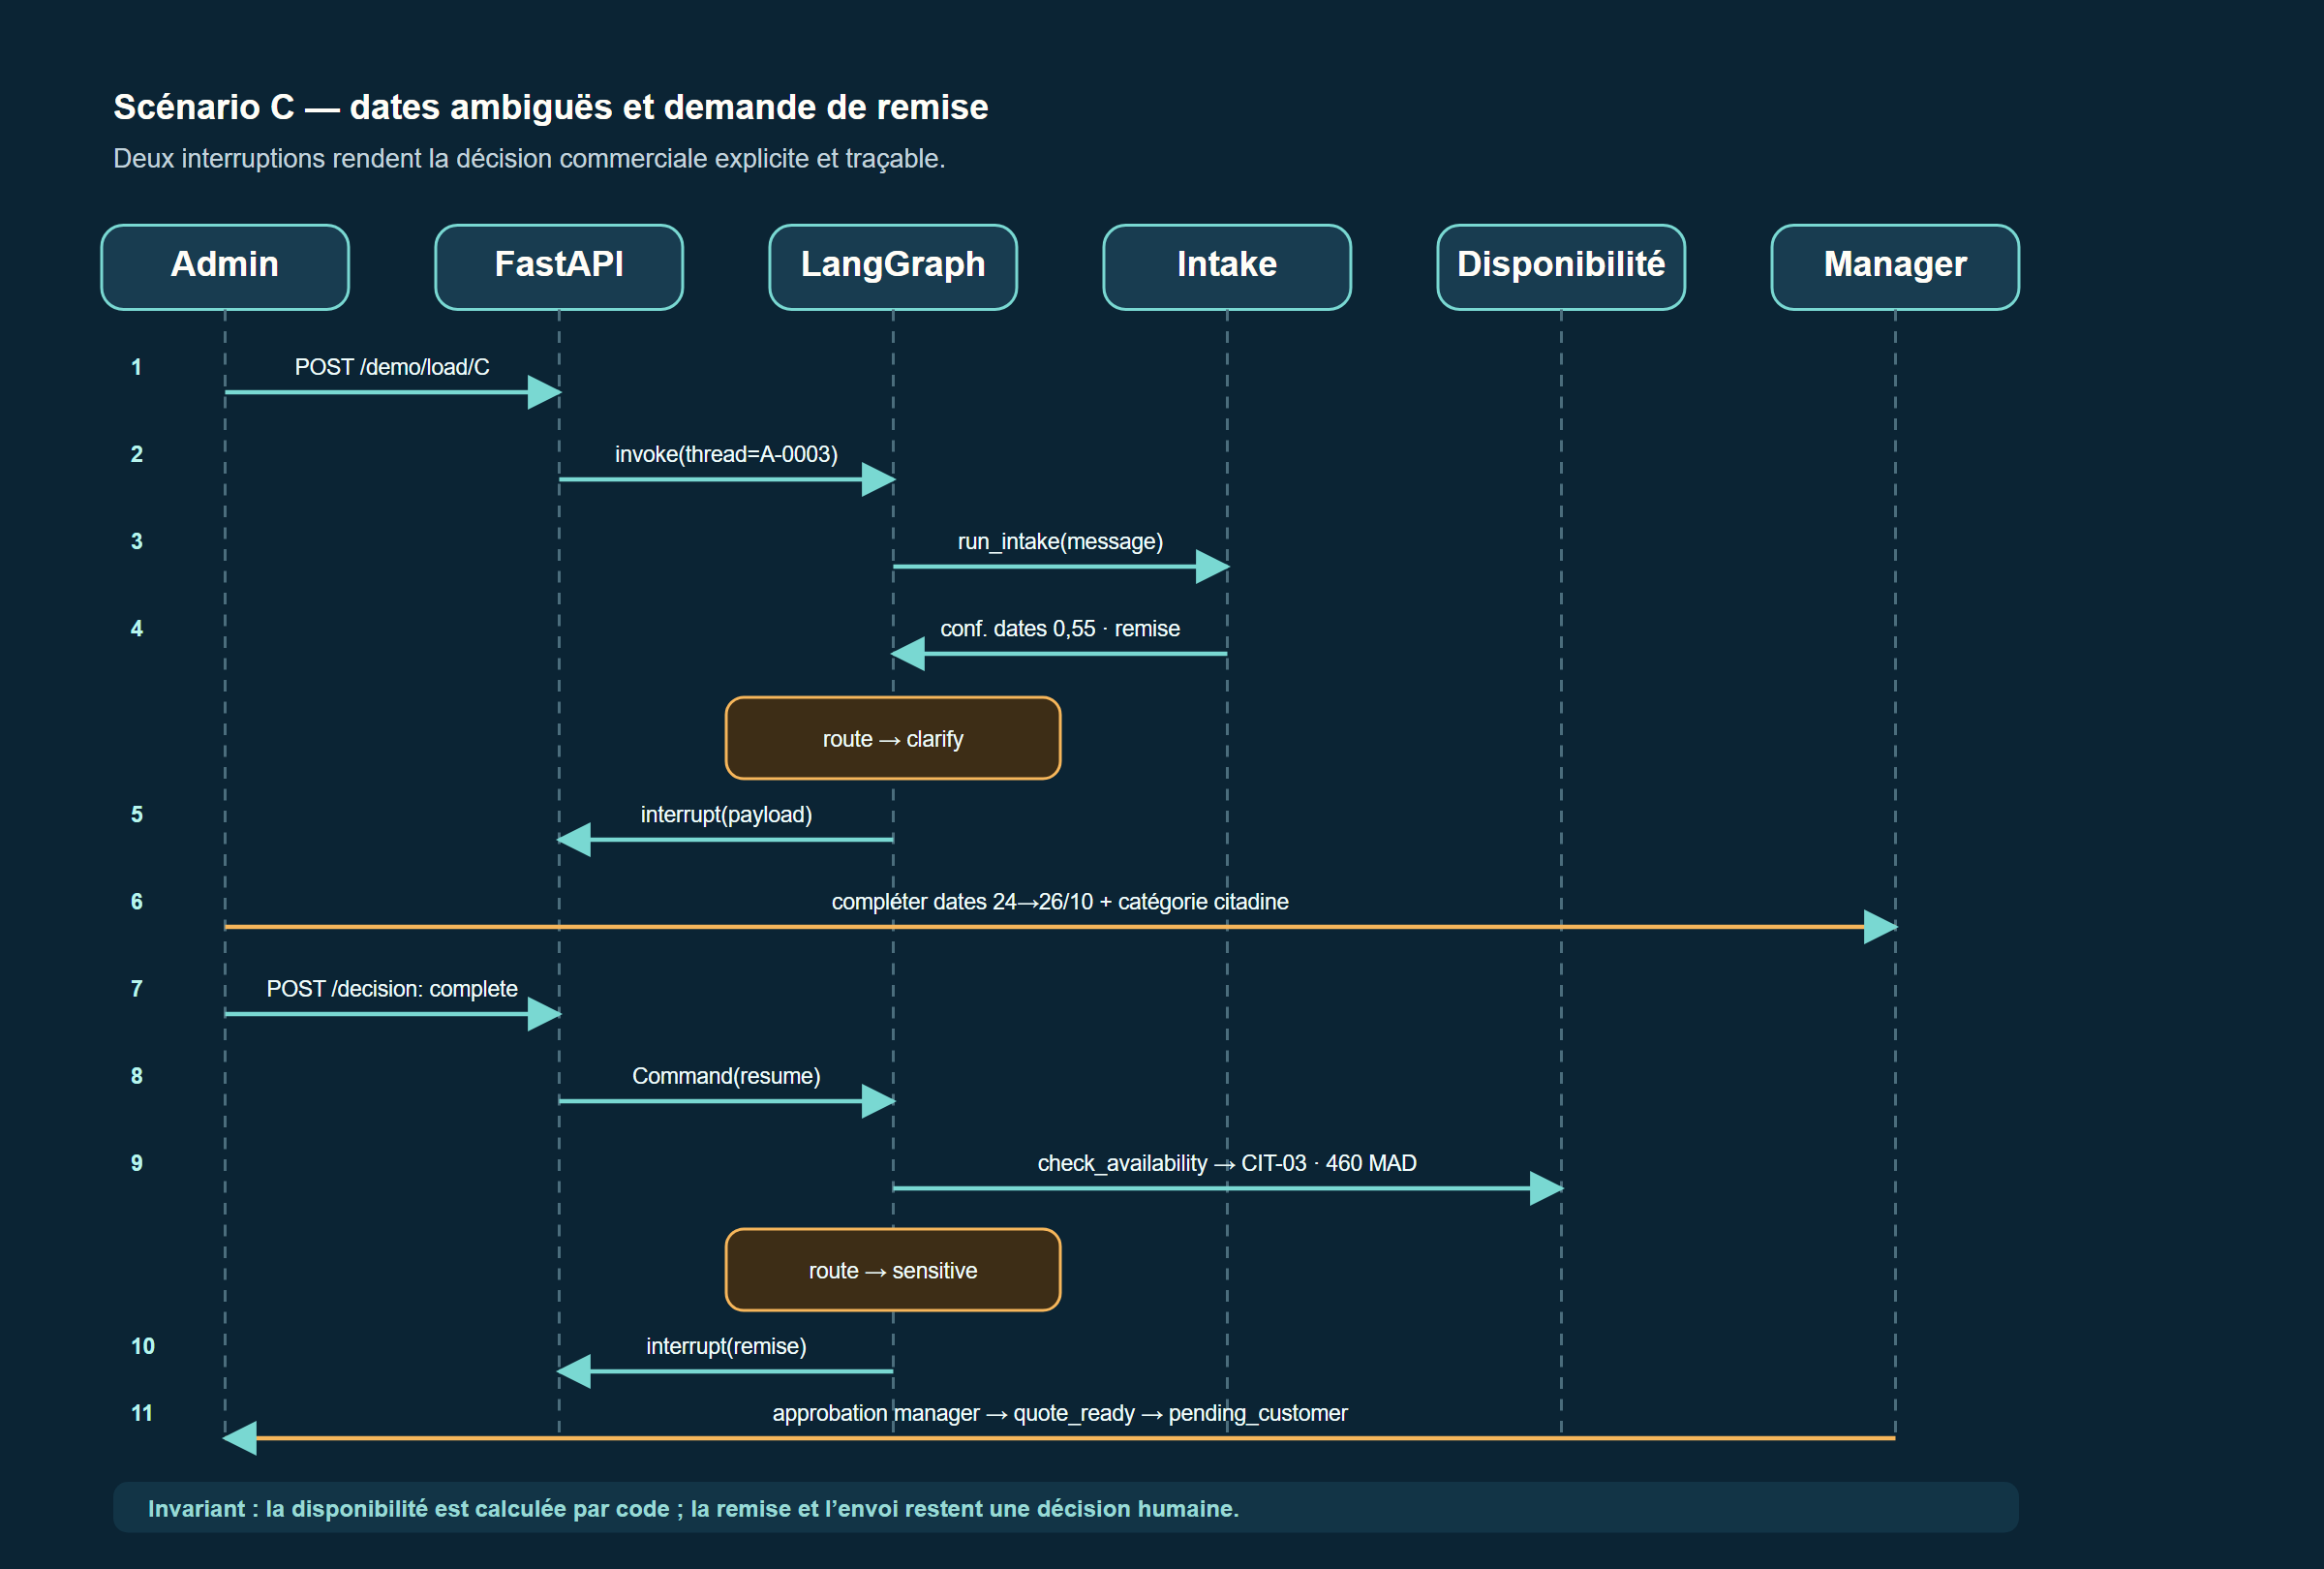
\includegraphics[width=0.95\linewidth]{fig_sequence_scenario_c.png}
\caption{Diagramme de sequence du scenario C. Deux \texttt{interrupt()} successifs : le premier pour clarifier les dates, le second pour valider la remise au niveau manager. Chaque etape ecrit un evenement dans la base.}
\label{fig:sequence-c}
\end{figure}

\section{Vue deploiement}

Trois topologies de deploiement sont supportees : (1) laptop hors ligne pour la demo agence ; (2) frontend Vercel/Netlify + backend Docker sur Render/Railway/Fly avec volume persistant ; (3) tout-Vercel serverless avec base Postgres externalisee (Neon ou Supabase).

\begin{figure}[H]\centering
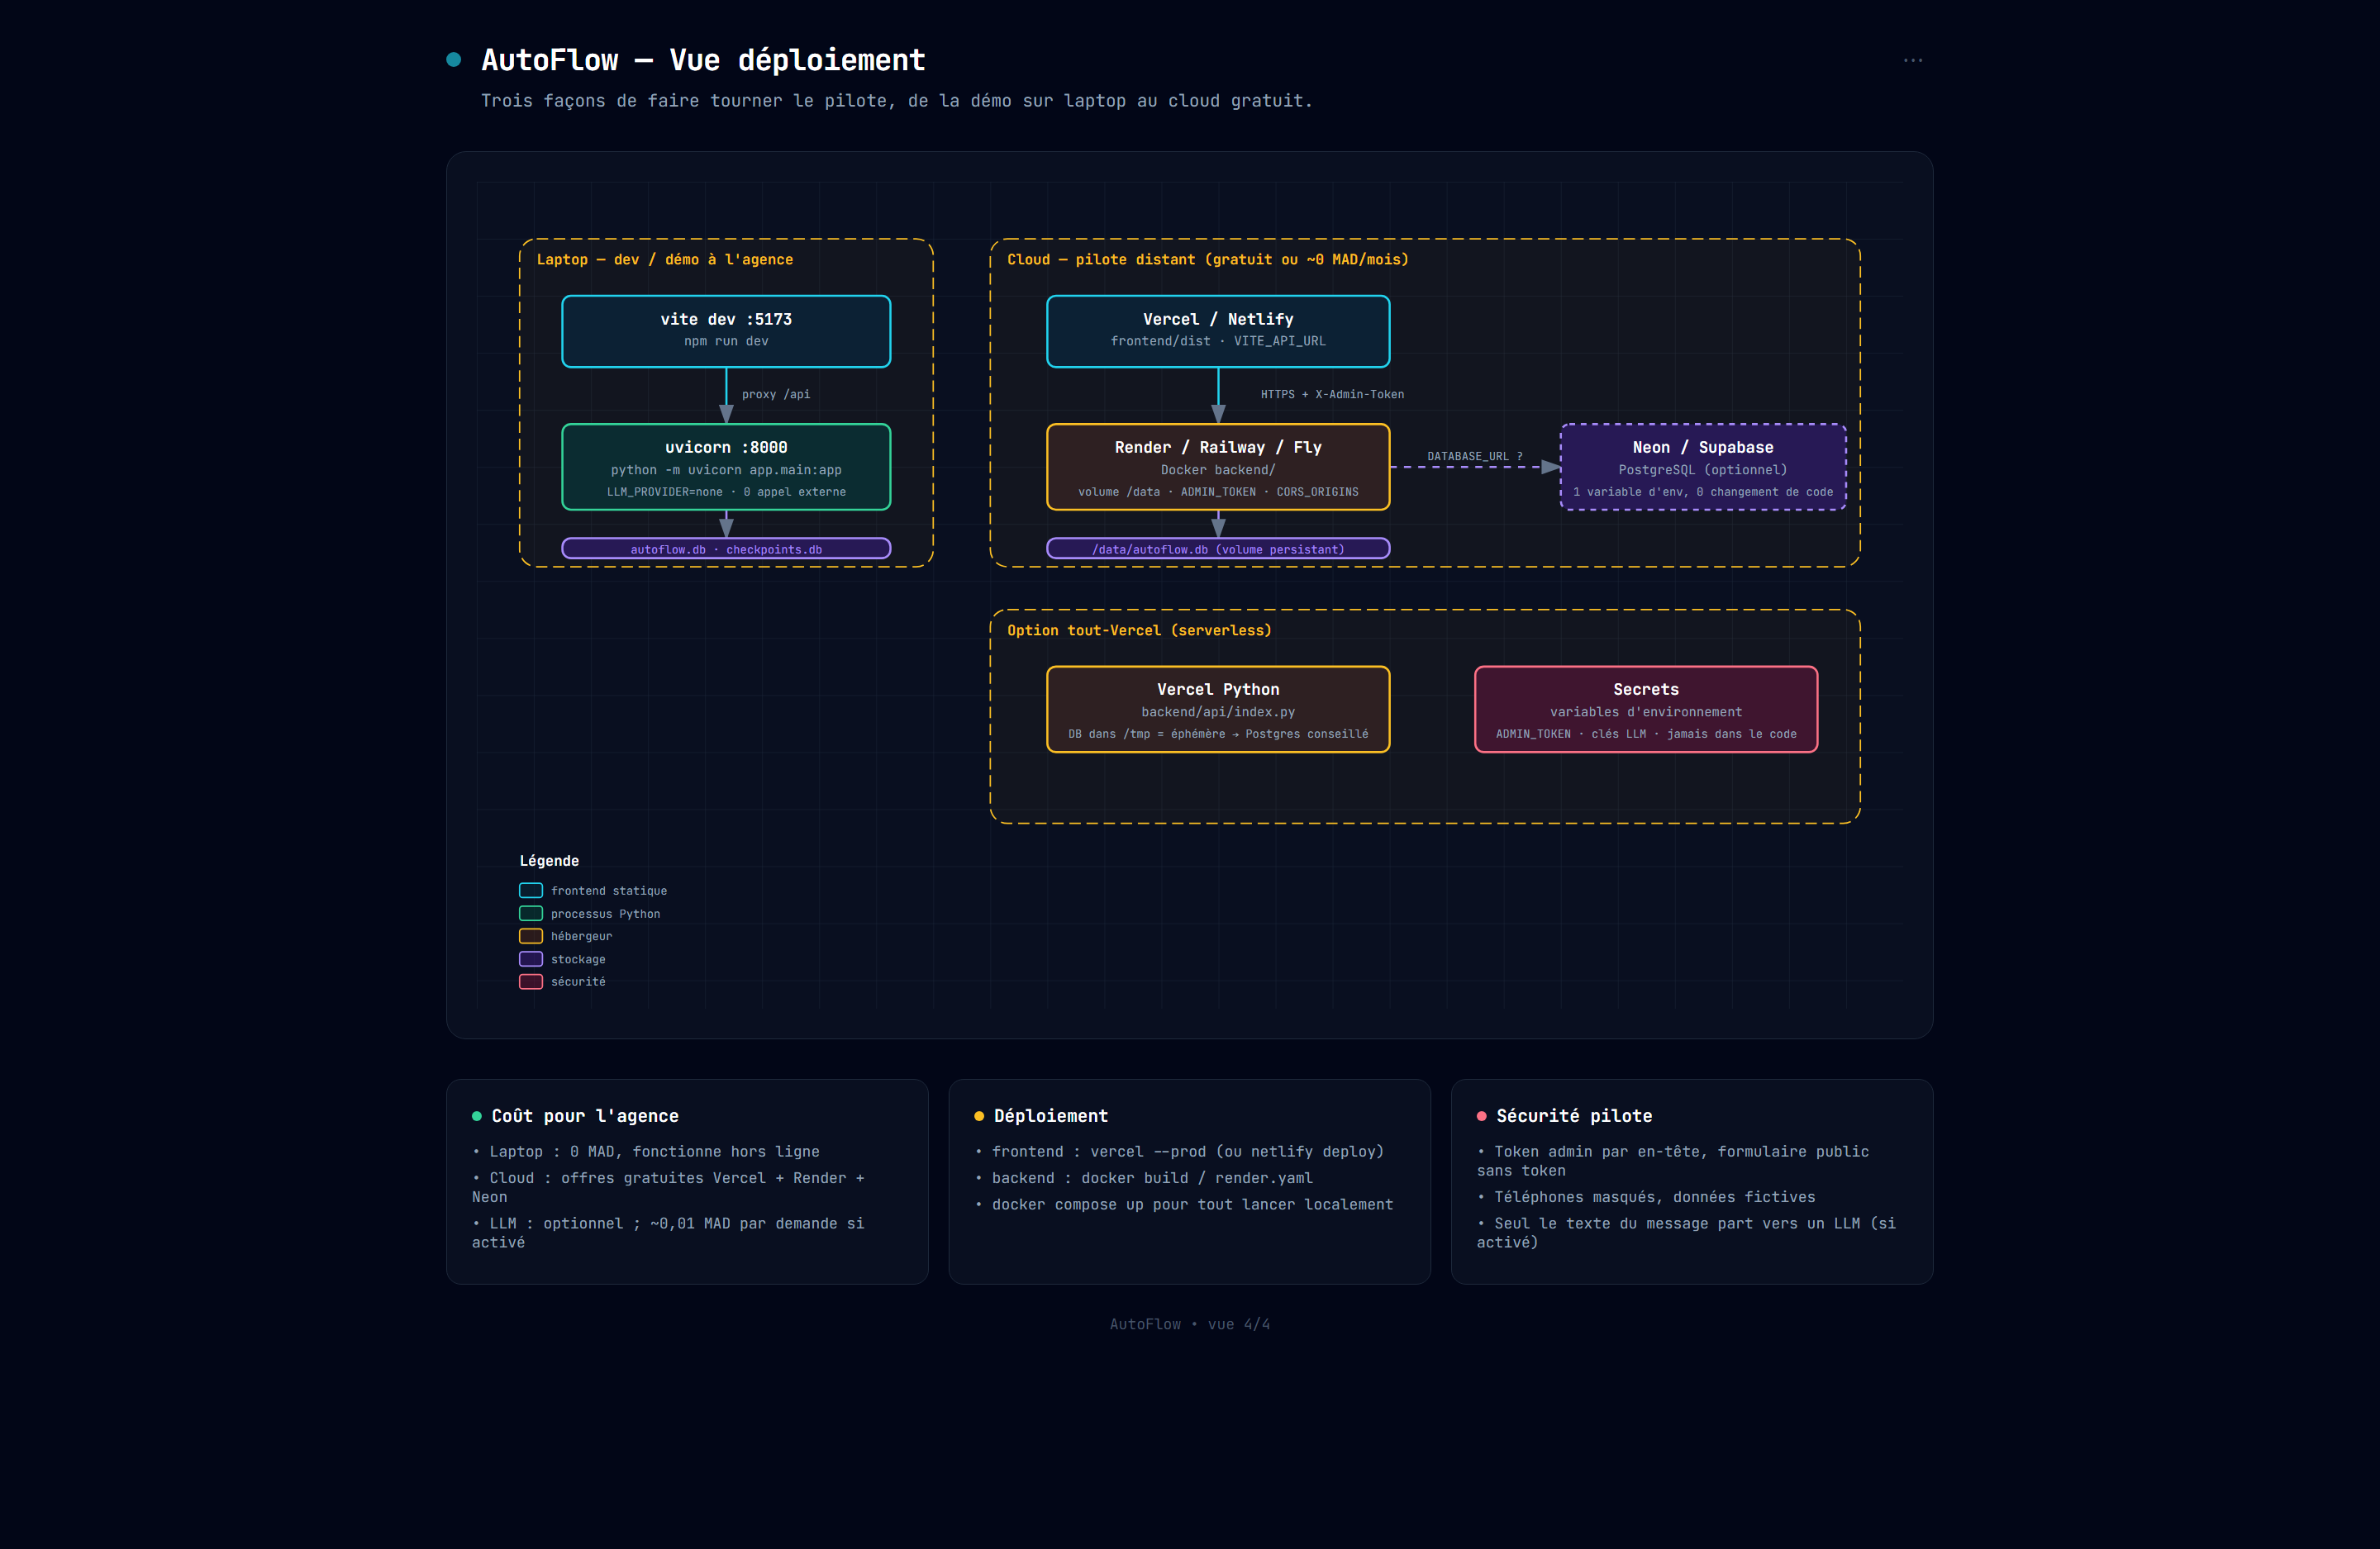
\includegraphics[width=0.95\linewidth]{fig_c4_deploiement.png}
\caption{Trois topologies de deploiement. Les secrets (\texttt{ADMIN\_TOKEN}, cles LLM) sont exclusivement en variables d'environnement ; le frontend ne contient aucun secret.}
\label{fig:c4-deploiement}
\end{figure}

\section{Vue defaillances}

\begin{table}[H]\centering\small
\caption{Vue defaillances --- comportement du systeme sous stress.}
\label{tab:defaillances}
\rowcolors{2}{softOrange}{white}
\begin{tabularx}{\textwidth}{X X X}\toprule
\rowcolor{boxOrange!30}\textbf{Defaillance} & \textbf{Comportement} & \textbf{Chemin de secours}\\\midrule
LLM indisponible / cle invalide  & Flag \texttt{llm\_failed}, confiance $\times$ 0{,}9 & Regles seules (toujours calculees)\\
LLM invente un champ             & Champ rejete (\texttt{null}), confiance $= 0$ & Question de clarification\\
Dates ambigues (< week-end prochain >>) & \texttt{needs\_human} + brouillon de question & Equipe complete $\rightarrow$ \texttt{Command(goto)}\\
Crash pendant le workflow        & Checkpoint LangGraph par noeud & Reprise au dernier noeud persiste\\
Boucle agents (\texttt{hops > 8}) & Route \texttt{sensitive} $\rightarrow$ humain & ---\\
Transition d'etat illegale       & \texttt{IllegalTransition} $\rightarrow$ HTTP 409 & Rien n'est ecrit\\
Trop de relances (\texttt{max\_reminders = 2}) & \texttt{stalled} $\rightarrow$ appel recommande & ---\\
\bottomrule
\end{tabularx}
\end{table}

\section{Conclusion}

L'architecture d'AutoFlow est desormais entierement specifiee : sept vues C4 complementaires, une machine a dix etats, une matrice d'escalade explicite, un modele de donnees derive du journal d'evenements. Cette architecture respecte les trois invariants (aucun envoi seul, aucune information inventee, tout trace) et satisfait toutes les exigences du chapitre~3. Le chapitre suivant en decrit la realisation, agent par agent.

% ================================================================
\chapter{Realisation : Agents et Orchestrateur}\label{chap:realisation1}
% ================================================================
Ce chapitre decrit la realisation logicielle du coeur du systeme : les trois agents specialises (Intake, Disponibilite, Suivi) et l'orchestrateur LangGraph qui les coordonne. Il commente les choix d'implementation, expose les extraits de code determinants, decrit le mecanisme du checkpointer et explique comment la validation humaine est materialisee par \texttt{interrupt()} et \texttt{Command}.

\section{Introduction}
La realisation du coeur backend represente environ 1400 lignes de Python metier, reparties en modules courts a responsabilite unique. Le principe << une fonction, une responsabilite >> est applique strictement : chaque agent est independamment testable et remplacable. Ce chapitre parcourt les composants dans l'ordre de leur execution par l'orchestrateur.

\section{Organisation du code}

\begin{lstlisting}[caption={Arborescence du backend AutoFlow.}]
backend/
  app/
    main.py            # FastAPI, 24 routes, auth token
    db.py              # SQLAlchemy 2.0, TRANSITIONS legales
    clock.py           # Horloge demo (avance controlee du temps)
    rules.py           # Chargement de rules.json
    agents/
      intake.py        # Comprendre : regles + LLM optionnel
      availability.py  # Verifier : deterministe, aucun LLM
      followup.py      # Preparer : brouillons + relances
    workflow/
      graph.py         # Orchestrateur LangGraph (StateGraph)
      orchestrator.py  # submit, resume, sweep, kpis, seed
      store.py         # transition, log, get_events, drafts
      explain.py       # Reconstruction du raisonnement
      state.py         # WorkflowState (TypedDict)
    simulations.py     # 7 cas metier, catalogue + runner
  data/
    generate_dataset.py, fleet.csv, bookings.csv,
    customers.csv, history.json, scenarios.json, rules.json
  tests/               # 16 tests (8 e2e + 7 sim + auth)
  eval/                # eval_intake.py, report.md
\end{lstlisting}

\section{Agent Intake --- comprendre le message}

\subsection{Le moteur de regles (toujours execute)}
L'agent Intake est double : un moteur de \textbf{regles} (regex, grammaire de dates FR/darija, lexiques) est toujours execute, et un moteur \textbf{LLM optionnel} peut le completer. Cette double execution permet a AutoFlow de tourner hors ligne et rend le LLM non critique.

\begin{lstlisting}[language=Python, caption={Extrait de \texttt{agents/intake.py} --- la boucle de fusion des deux moteurs.}]
def run_intake(message: str) -> StructuredRequest:
    normalised = normalise_nfd(message)
    rules_out = extract_rules(normalised)      # deterministe
    if not llm_enabled():
        return _finalise(rules_out, engine="rules")
    try:
        llm_out = extract_llm(normalised)       # avec evidence gate
    except Exception as exc:
        return _finalise(rules_out, engine="rules",
                         flags=[f"llm_failed:{type(exc).__name__}"])
    fused = fuse(rules_out, llm_out)           # accord -> 0.95 ;
    return _finalise(fused, engine="rules+llm") # sinon LLM avec preuve
\end{lstlisting}

\subsection{L'evidence gate}
Le mecanisme central de l'agent Intake est l'\emph{evidence gate}. Apres extraction par le LLM (via \texttt{with\_structured\_output}), chaque champ est verifie : le passage justificatif (\texttt{evidence[k]}) doit etre une sous-chaine exacte du message normalise. Sinon, le champ est \textbf{rejete}.

\begin{alertbox}[Anti-hallucination structurelle]
Si le LLM propose \texttt{return\_date = "2026-10-27"} et \texttt{evidence["return\_date"] = "le 27 octobre au soir"} mais que cette chaine n'est \emph{pas} presente dans le message brut, le champ est \textbf{rejete}. La demande passe alors en clarification humaine. Aucune date fantome ne peut sortir de l'agent.
\end{alertbox}

\subsection{Les signaux typés}
Enfin, l'agent Intake expose des \texttt{signals} : des probabilites calibrees sur des questions oui/non binaires, que l'orchestrateur compare a des seuils. Cette representation \emph{numerique} des decisions --- inspiree de Jev AI --- supprime la principale source de fragilite des orchestrateurs << conversationnels >>.

\section{Agent Disponibilite --- verifier sans LLM}

L'agent Disponibilite est \textbf{intentionnellement deterministe} : aucun appel LLM. Il resoud le probleme du chevauchement des reservations avec un tampon de 4 heures (nettoyage + reprise), filtre les vehicules en maintenance, propose des \emph{replis} par categorie (\texttt{category\_fallbacks}) et des \emph{decalages} de dates (\texttt{shift\_days\_allowed}, $\pm$3 jours). Chaque option ecartee porte une \textbf{raison lisible}.

\begin{mechanismbox}[L'argument n{\textdegree}1 de confiance pour le gerant]
L'agent Disponibilite ne peut \emph{pas} inventer un vehicule libre : sa logique est du SQL et de la comparaison de dates. Cet argument est central dans la vente au gerant : << c'est du code, pas une IA. Si le vehicule est reserve, le systeme le dit ; il ne peut pas se tromper. >>
\end{mechanismbox}

\section{Agent Suivi --- preparer sans envoyer}

L'agent Suivi produit trois types de brouillons FR : \emph{devis} (avec prix injecte depuis la table \texttt{vehicles}), \emph{alternative} (quand une option a ete substituee) et \emph{clarification} (quand une question doit etre posee). Il applique une \emph{politique de relance} : la premiere relance est planifiee a +24~h de l'envoi initial, un maximum de deux relances est autorise, et un lead sans reponse depuis 72~h passe en \texttt{stalled} avec recommandation d'appel.

\begin{lstlisting}[language=Python, caption={Extrait de \texttt{agents/followup.py} --- template de devis avec prix injecte.}]
def draft_quote(structured: StructuredRequest, avail: AvailabilityResult) -> str:
    option = avail.options[0]  # meilleure option classee
    vehicle = fleet.get(option.vehicle_id)
    total = option.days * vehicle.price_per_day
    return TEMPLATES["devis"].format(
        client_first_name=structured.client.first_name or "",
        vehicle_label=f"{vehicle.brand} {vehicle.model}",
        days=option.days,
        price_per_day=vehicle.price_per_day,   # jamais genere
        total=total,
        pickup_site=option.pickup_site,
    )
\end{lstlisting}

\section{Orchestrateur LangGraph --- coordonner et suspendre}

\subsection{Structure du graphe}
L'orchestrateur est un \texttt{StateGraph} LangGraph avec sept noeuds (\texttt{intake}, \texttt{escalate}, \texttt{clarify}, \texttt{availability}, \texttt{sensitive}, \texttt{draft}, \texttt{human\_review}, \texttt{finalize}) et deux gardes conditionnelles.

\begin{lstlisting}[language=Python, caption={Extrait de \texttt{workflow/graph.py} --- garde de routage apres Intake.}]
def route_after_intake(state: WorkflowState) -> str:
    s = state["structured"]
    if s.signals.get("is_complaint", 0.0) >= rules["complaint_threshold"]:
        return "escalate"
    if s.missing or s.confidence < rules["confidence_threshold"]:
        return "clarify"
    critical = min(s.field_confidence.get(f, 1.0)
                   for f in rules["critical_fields"])
    if critical < rules["critical_field_threshold"]:
        return "clarify"
    return "availability"
\end{lstlisting}

\subsection{Le point d'interruption humain}
Le noeud \texttt{human\_review} est un \texttt{interrupt()} reel : l'execution est suspendue, le payload persiste par le checkpointer, et l'API expose cet etat comme \texttt{pending\_interrupt}. La reprise se fait par \texttt{Command(resume=decision)} pour approuver/modifier/refuser/cloturer, ou \texttt{Command(goto="availability")} apres completion des champs manquants.

\subsection{Le checkpointer SQLite}
Le \texttt{SqliteSaver} de LangGraph persiste l'etat du graphe (variables, position dans le graphe, payload d'interruption) apres chaque noeud dans une base dediee (\texttt{checkpoints.db}). Consequence directe : \textbf{une validation en attente survit a un redemarrage} du serveur. Un test dedie (\texttt{test\_kpis\_and\_graph}) verifie cette propriete.

\begin{figure}[H]\centering
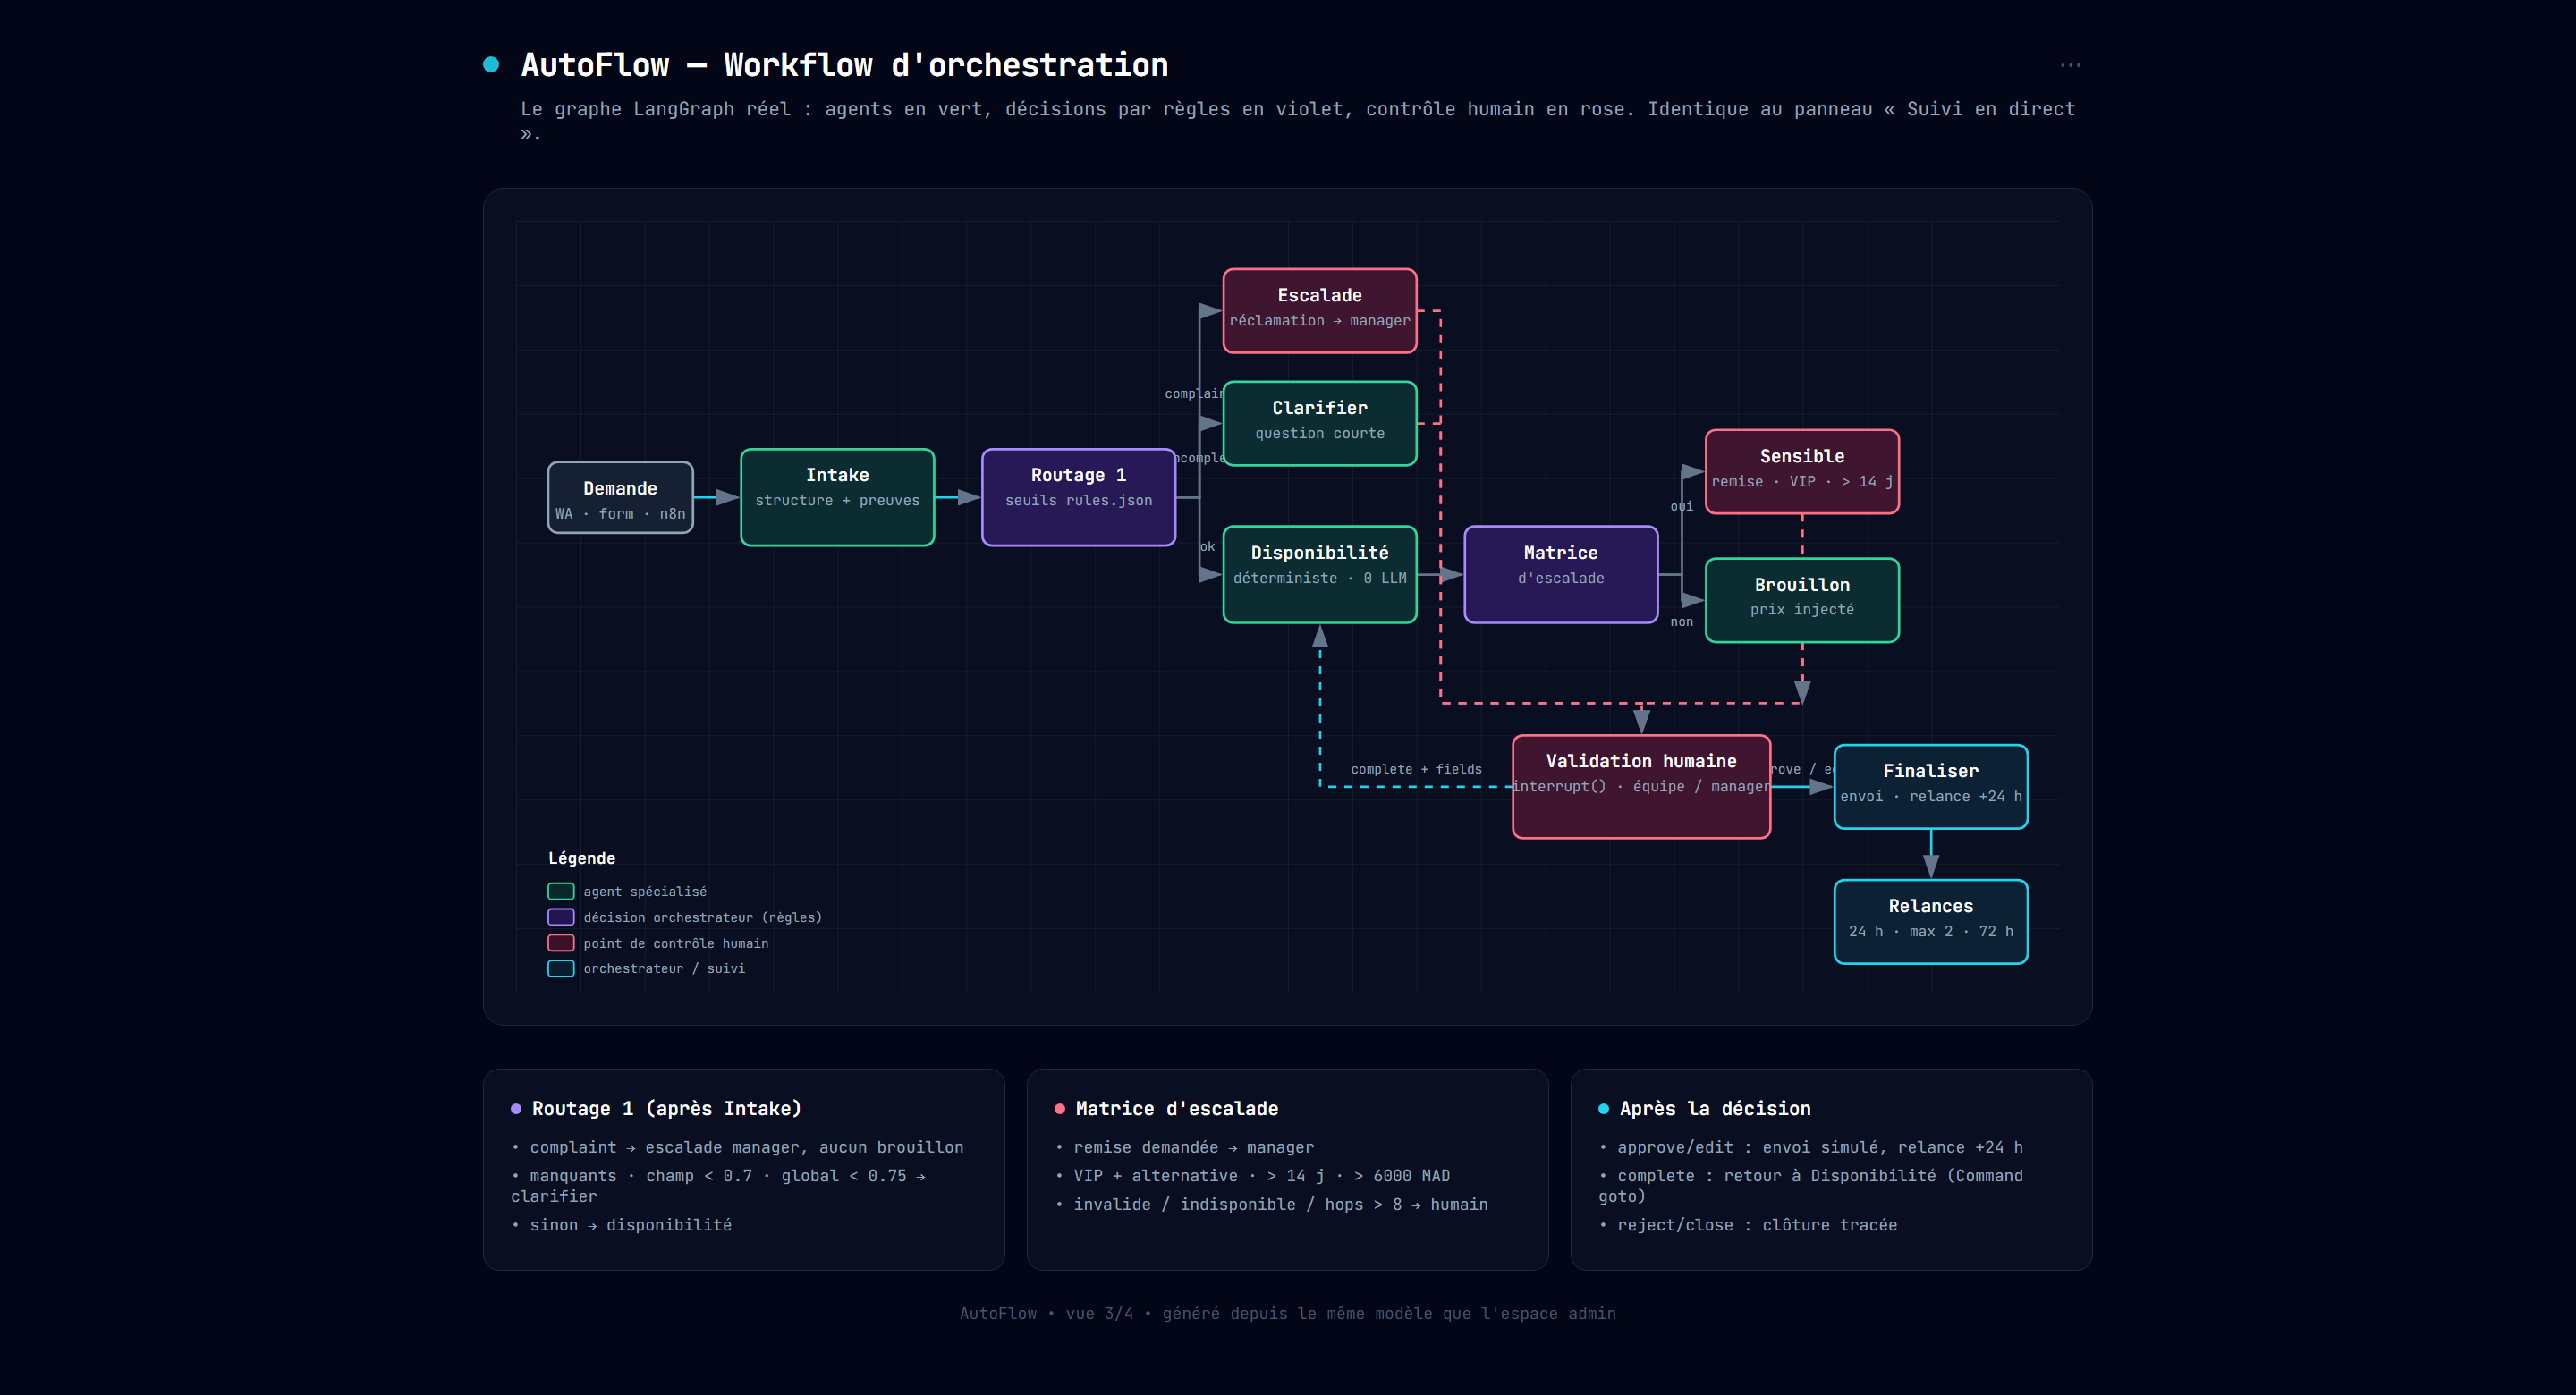
\includegraphics[width=0.95\linewidth]{fig_graphe_langgraph.png}
\caption{Rappel visuel du graphe d'orchestration (cf. chapitre~4). Le noeud \texttt{human\_review} est le point de suspension persiste.}
\end{figure}

\section{Difficultes rencontrees et resolutions}

\begin{itemize}[leftmargin=1.5cm]
\item \textbf{Dates francaises ambigues} : la forme << du 27 aout au 17 septembre >> prenait le second mois pour les deux dates. Correction : ajout d'une capture optionnelle du premier mois dans le regex. Detection : evaluation quantitative de l'agent Intake.
\item \textbf{Horloge de lead sans reponse} : elle repartait a chaque relance envoyee, rendant \texttt{stalled} inatteignable apres la deuxieme relance. Correction : prendre pour reference la \emph{premiere reponse envoyee}. Detection : simulation << lead silencieux >>.
\item \textbf{Priorite d'intention} : << je passerai reserver plus tard >> faisait primer \emph{reservation} sur \emph{information}. Correction : regle ajoutee (question sans date + mots d'information $\rightarrow$ \texttt{info}). Detection : simulation << question d'information >>.
\item \textbf{Fichiers SQLite verrouilles sous Windows} dans les tests : liberation explicite de l'engine et du cache du graphe entre chaque test.
\end{itemize}

\section{Conclusion}

Les trois agents et l'orchestrateur constituent le coeur executable d'AutoFlow. Leur implementation respecte strictement le principe de responsabilite unique, l'invariant << aucune information inventee >> (via l'evidence gate et le determinisme de la disponibilite) et l'invariant << aucun envoi seul >> (via \texttt{interrupt()}). Le chapitre suivant presente les couches externes : API REST, espace d'administration React et integrations n8n.

% ================================================================
\chapter{Realisation : API, Espace Admin, Integrations}\label{chap:realisation2}
% ================================================================
Ce chapitre couvre les couches en peripherie du coeur decrit au chapitre~5 : l'API REST FastAPI qui expose l'orchestrateur, l'espace d'administration React qui materialise la validation humaine, les integrations n8n en peripherie, le generateur de donnees realistes et le catalogue de sept simulations metier.

\section{Introduction}
Un moteur de workflow, aussi bien concu soit-il, reste invisible sans les surfaces qui l'exposent. Ce chapitre presente les quatre surfaces qui rendent AutoFlow utilisable et demontrable : l'API JSON, l'espace admin, les integrations peripheriques et le systeme de donnees realistes.

\section{API REST FastAPI}

L'API expose \textbf{24 routes} organisees en huit familles : \texttt{/api/health}, \texttt{/api/public/*} (formulaire client, ingestion webhook n8n), \texttt{/api/requests/*} (CRUD demandes, decision humaine), \texttt{/api/trace/*} (raisonnement, journal), \texttt{/api/live/*} (flux d'evenements), \texttt{/api/reviews/*} (file), \texttt{/api/fleet/*} et \texttt{/api/rules/*} (parametres), \texttt{/api/kpis}, \texttt{/api/events}, \texttt{/api/graph}, \texttt{/api/simulations/*}, \texttt{/api/demo/*} (scenarios, horloge, reset).

\begin{table}[H]\centering\small
\caption{Extrait des routes principales de l'API.}
\label{tab:routes}
\rowcolors{2}{softBlue}{white}
\begin{tabularx}{\textwidth}{l l X}\toprule
\rowcolor{boxBlue!30}\textbf{Methode} & \textbf{Route} & \textbf{Description}\\\midrule
\texttt{POST}  & \texttt{/api/public/intake}       & Ingestion d'un message client (formulaire ou webhook n8n)\\
\texttt{POST}  & \texttt{/api/requests/\{id\}/decision} & Decision humaine (approve, edit, reject, close, complete)\\
\texttt{GET}   & \texttt{/api/reviews}             & File des demandes a valider (equipe / manager)\\
\texttt{GET}   & \texttt{/api/trace/\{id\}}        & Reconstruction du raisonnement d'une demande\\
\texttt{GET}   & \texttt{/api/live/events}         & Flux d'evenements en temps quasi reel\\
\texttt{GET}   & \texttt{/api/graph}               & Diagramme Mermaid du graphe LangGraph\\
\texttt{GET}   & \texttt{/api/kpis}                & Compteurs agreges depuis le journal\\
\texttt{POST}  & \texttt{/api/demo/load/\{scenario\}} & Charge un scenario de demo (A--E)\\
\bottomrule
\end{tabularx}
\end{table}

L'authentification repose sur un \textbf{token unique} passe par en-tete \texttt{X-Admin-Token}. Le formulaire public \texttt{/demande} ne requiert pas ce token (uniquement en lecture). Le CORS est restreint a l'URL du frontend en production.

\section{Espace d'administration React}

\subsection{Vue d'ensemble}
L'espace admin est une SPA React 19 + Vite + TypeScript, construite en 10 ecrans, sans framework UI kit : uniquement du CSS custom aux couleurs de la charte (navy \#0B1F3A / teal \#0E9C99 / creme \#F7F4EC), avec Manrope comme police, icones SVG, transitions courtes, anneaux de focus, respect de \texttt{prefers-reduced-motion}.

\subsection{La file a valider}
L'ecran central est la \textbf{file a valider}. Chaque ligne montre l'identifiant, le niveau requis (badge equipe ou manager), la priorite, une raison lisible (<< Remise demandee --- validation manager >>), le brouillon prepare et trois boutons : \emph{Approuver \& envoyer}, \emph{Modifier}, \emph{Refuser}.

\begin{figure}[H]\centering
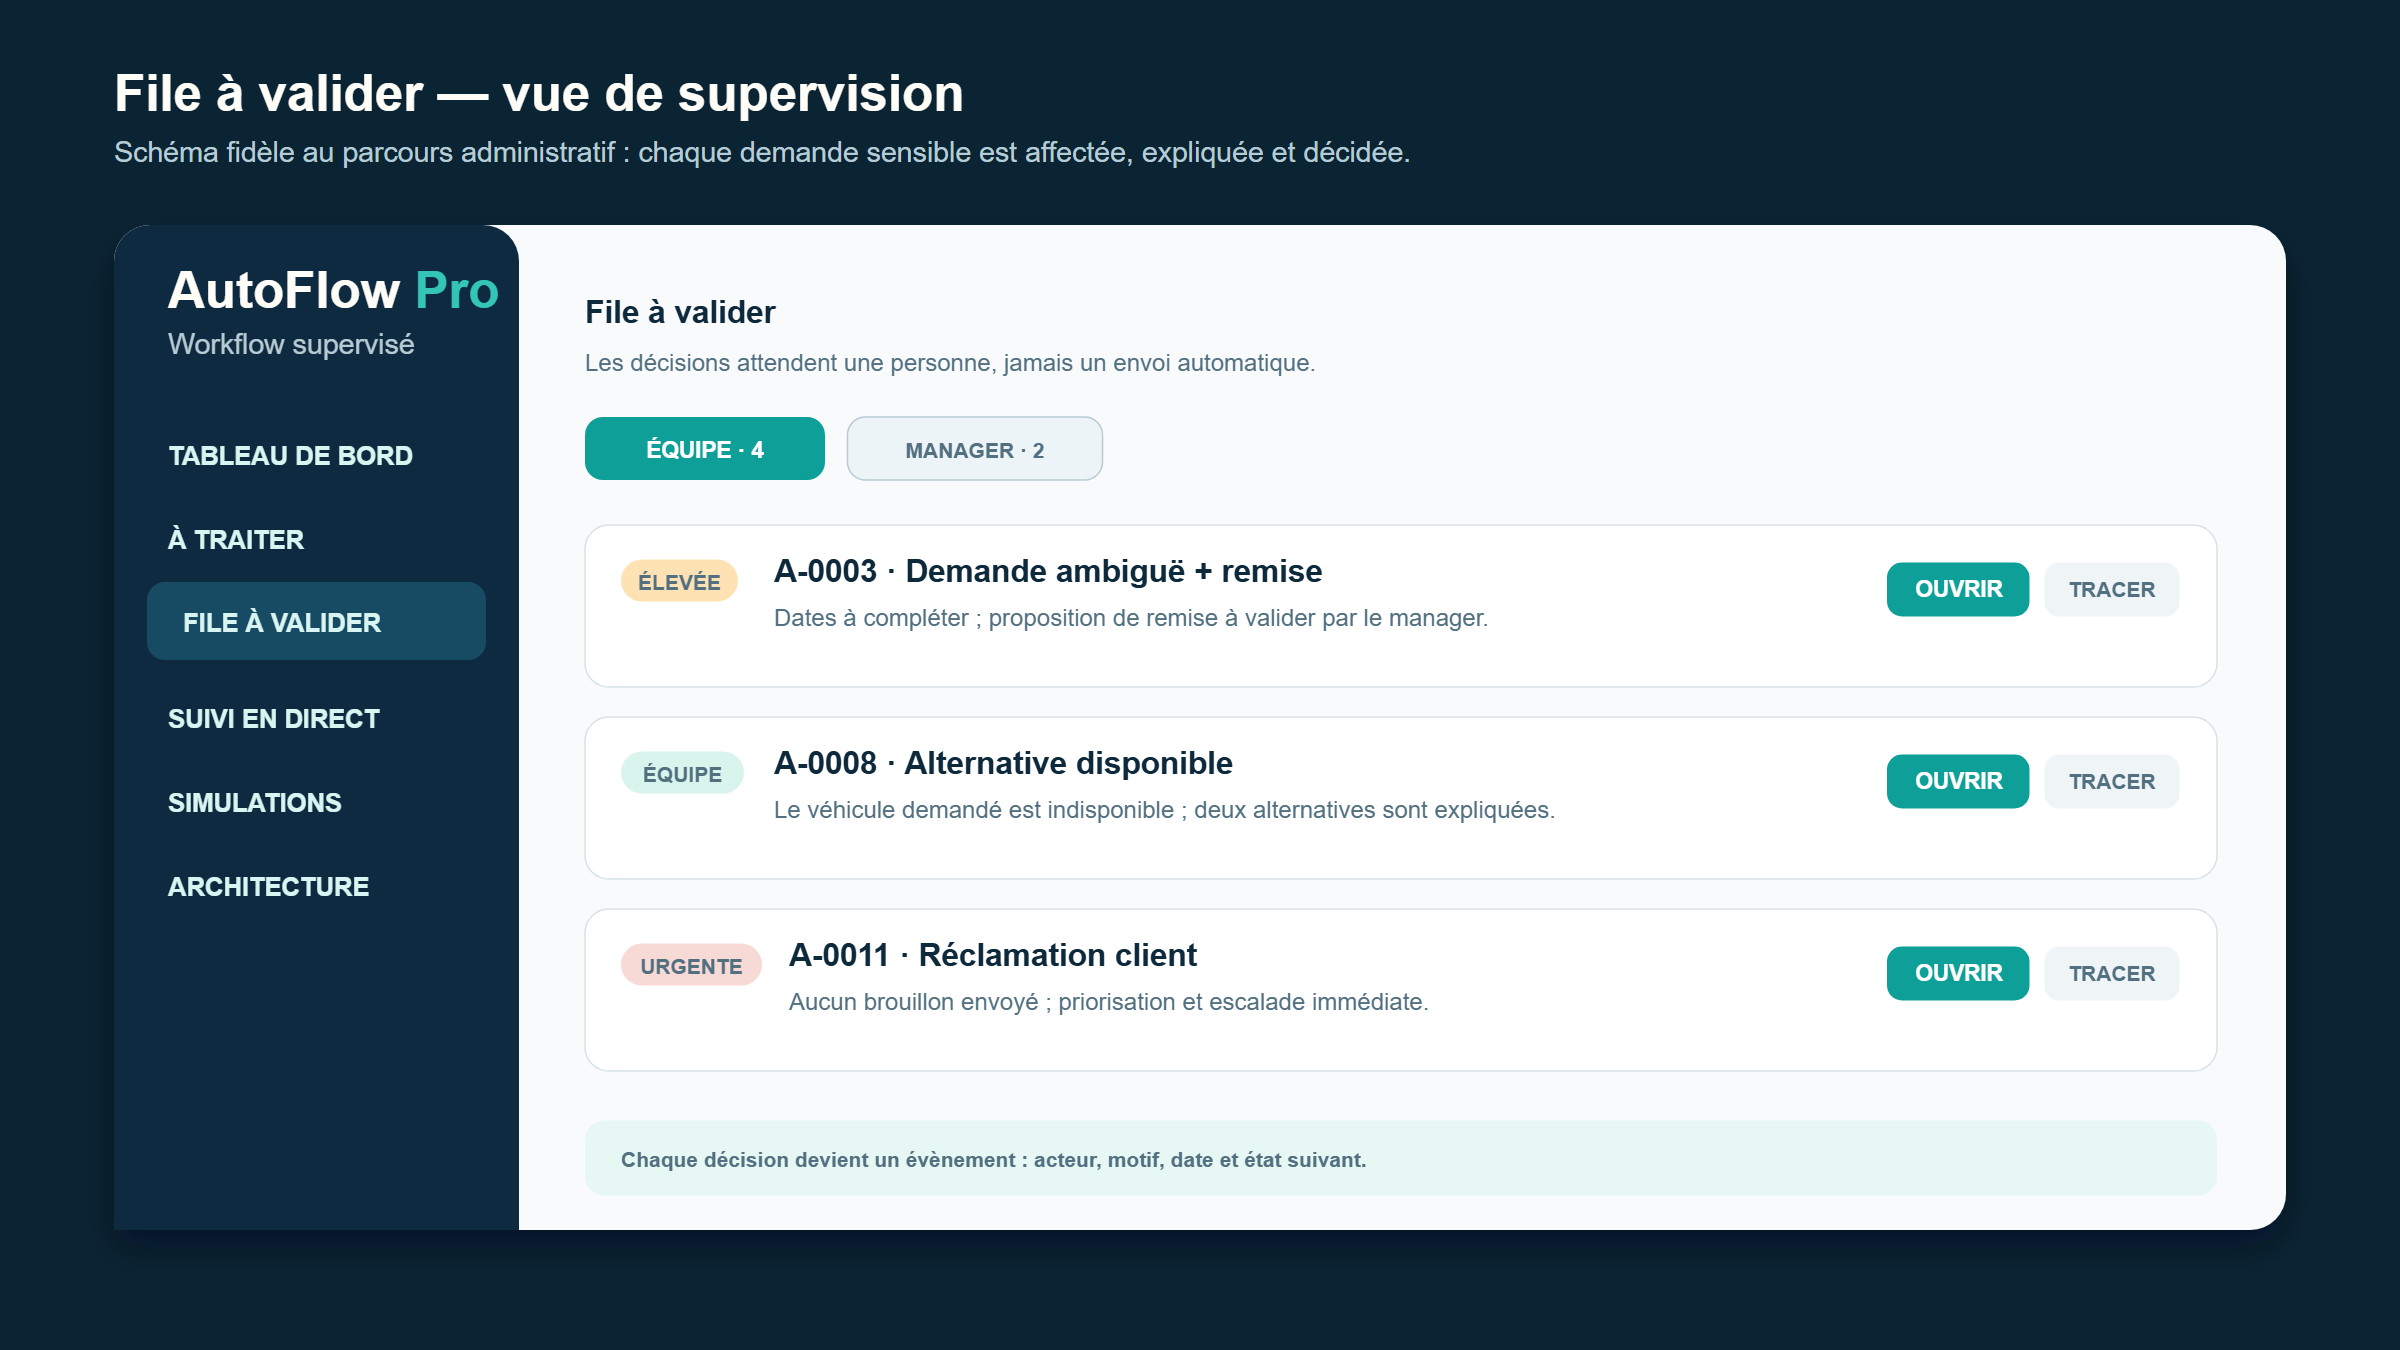
\includegraphics[width=0.95\linewidth]{fig_admin_queue.png}
\caption{Schema de la file a valider. La demande expose son niveau de revue, sa priorite, son motif et les actions disponibles avant toute sortie client.}
\label{fig:admin-queue}
\end{figure}

\subsection{Le suivi en direct et le raisonnement}
L'ecran \textbf{Suivi en direct} affiche un flux d'evenements en temps quasi reel (rafraichissement toutes les 4~s) et, pour toute demande selectionnee, deux panneaux critiques : (1) le graphe du workflow avec le \emph{chemin realement suivi allume} en teal ; (2) un tableau listant chaque regle evaluee (nom, valeur mesuree, seuil, branche declenchee).

\begin{figure}[H]\centering
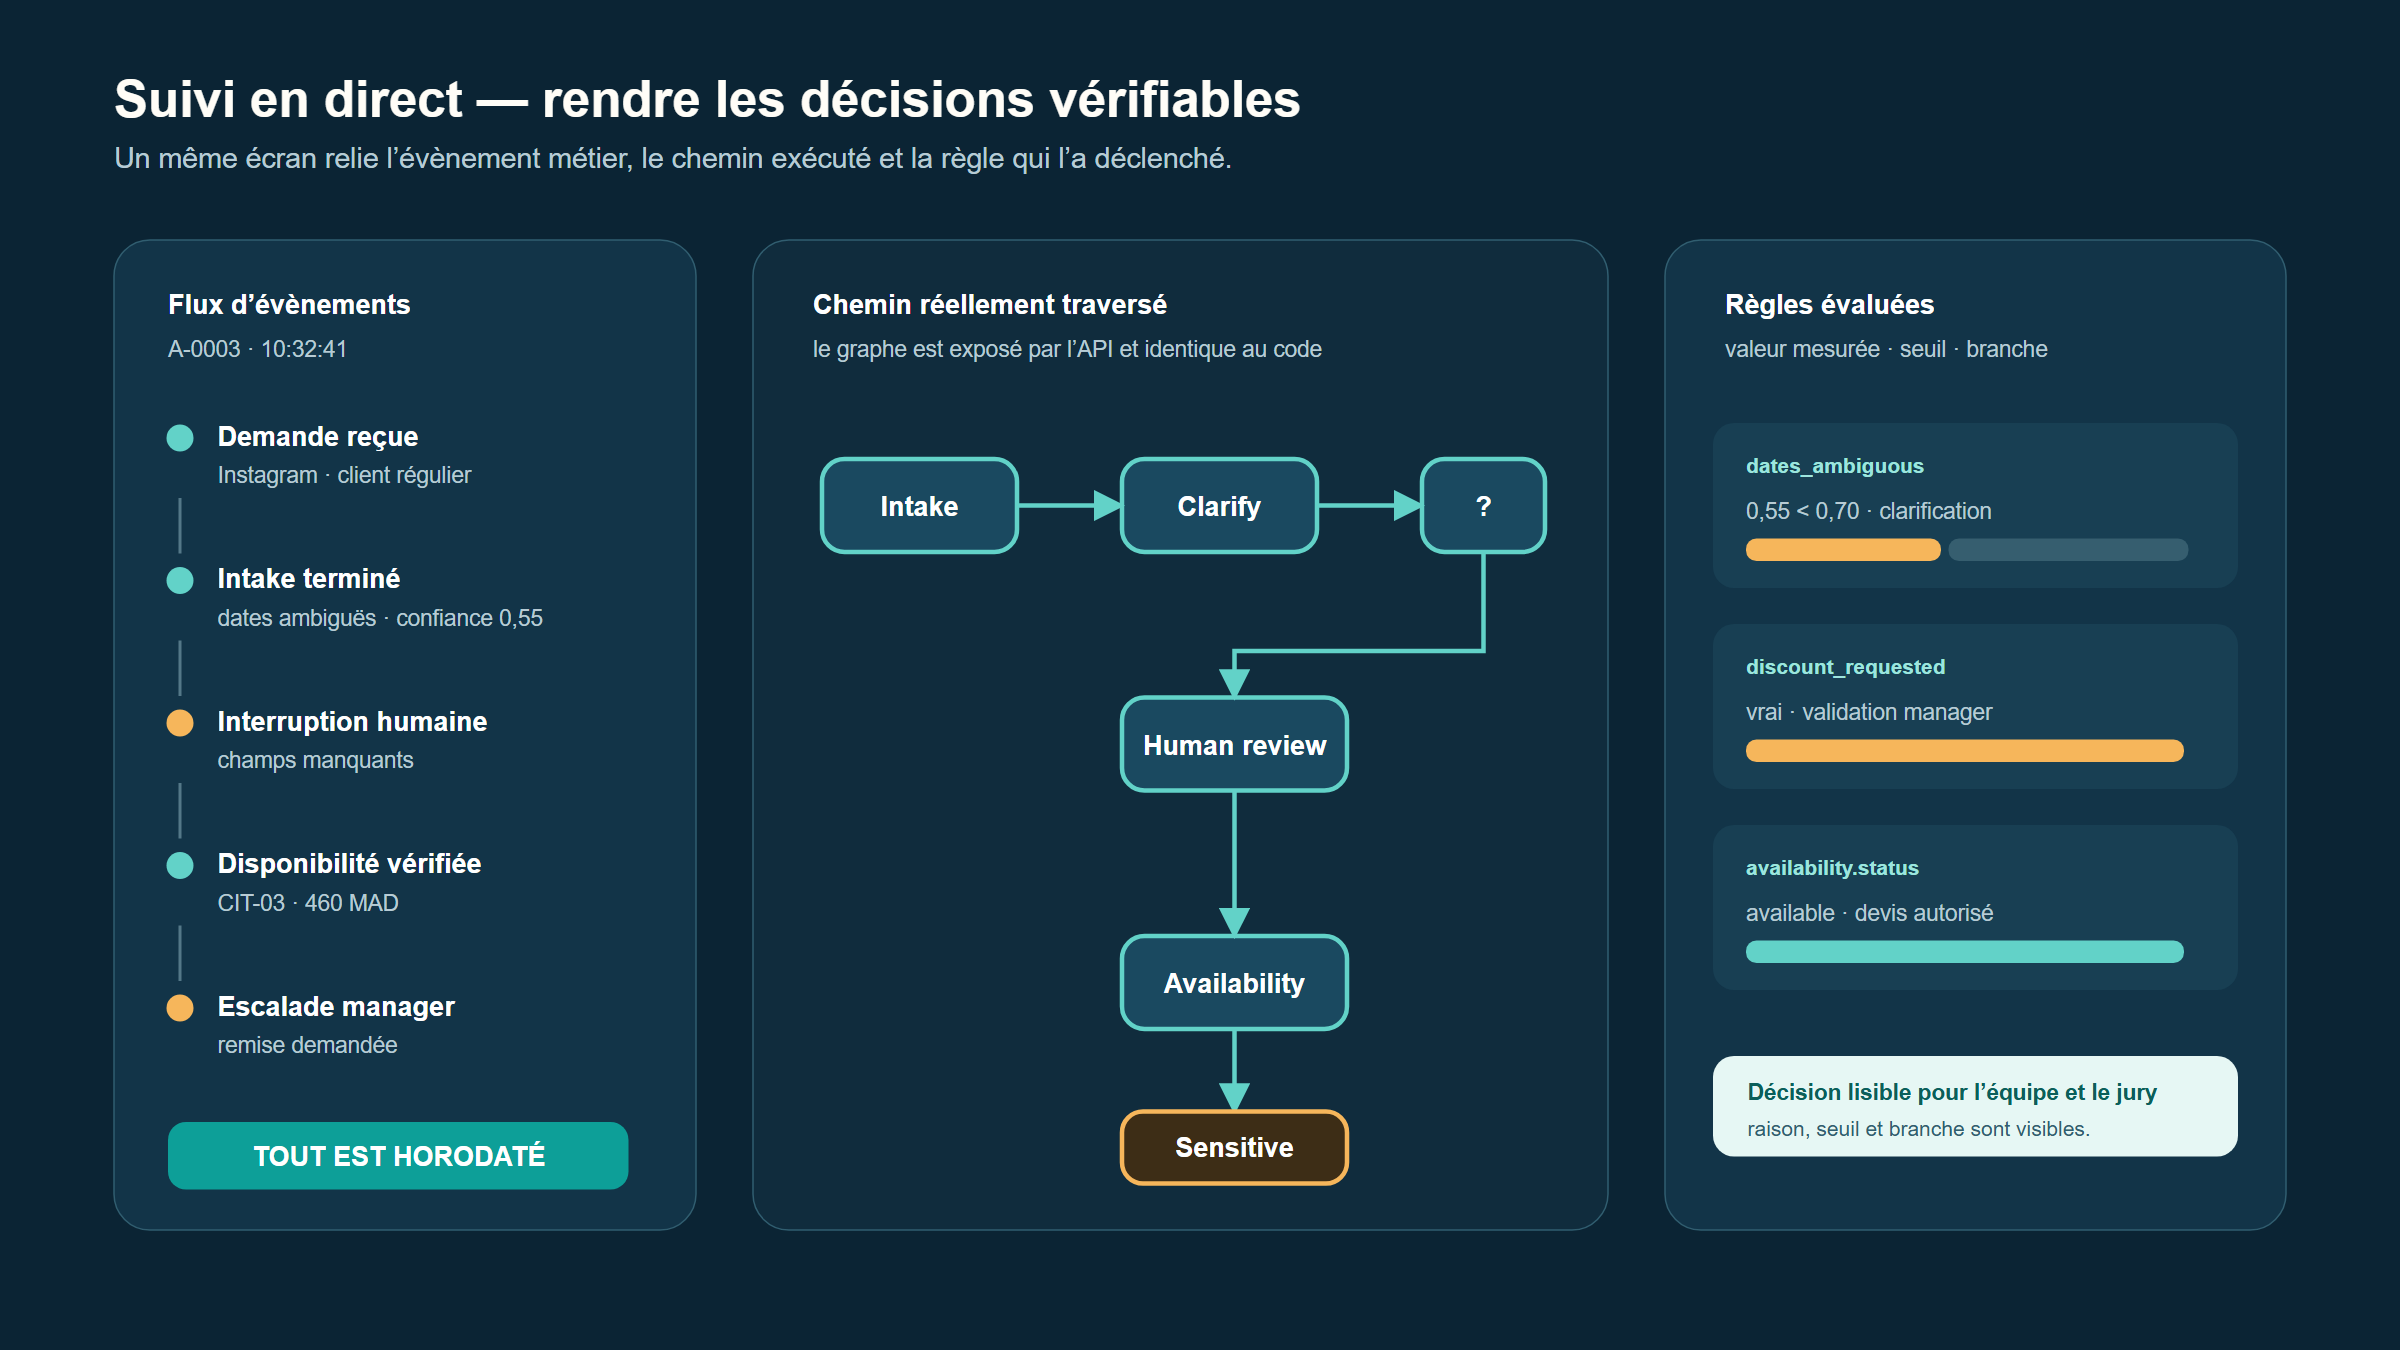
\includegraphics[width=0.95\linewidth]{fig_admin_live_trace.png}
\caption{Schema du suivi explicable : flux d'evenements, chemin execute et regles evaluees. Chaque decision est rattachee a une valeur, un seuil et une branche.}
\label{fig:admin-live}
\end{figure}

\subsection{Les simulations et le mode presentation}
Le menu \textbf{Simulations} propose sept cas metier scriptes joues \emph{a travers la vraie API}, avec revelation etape par etape (acteur, etat atteint, verifications $\checkmark$/$\times$). Les memes cas servent de tests d'acceptation en CI (\texttt{test\_simulations.py}). Le \textbf{Mode presentation} agrandit la typographie et masque les controles de demo pour la soutenance.

\begin{figure}[H]\centering
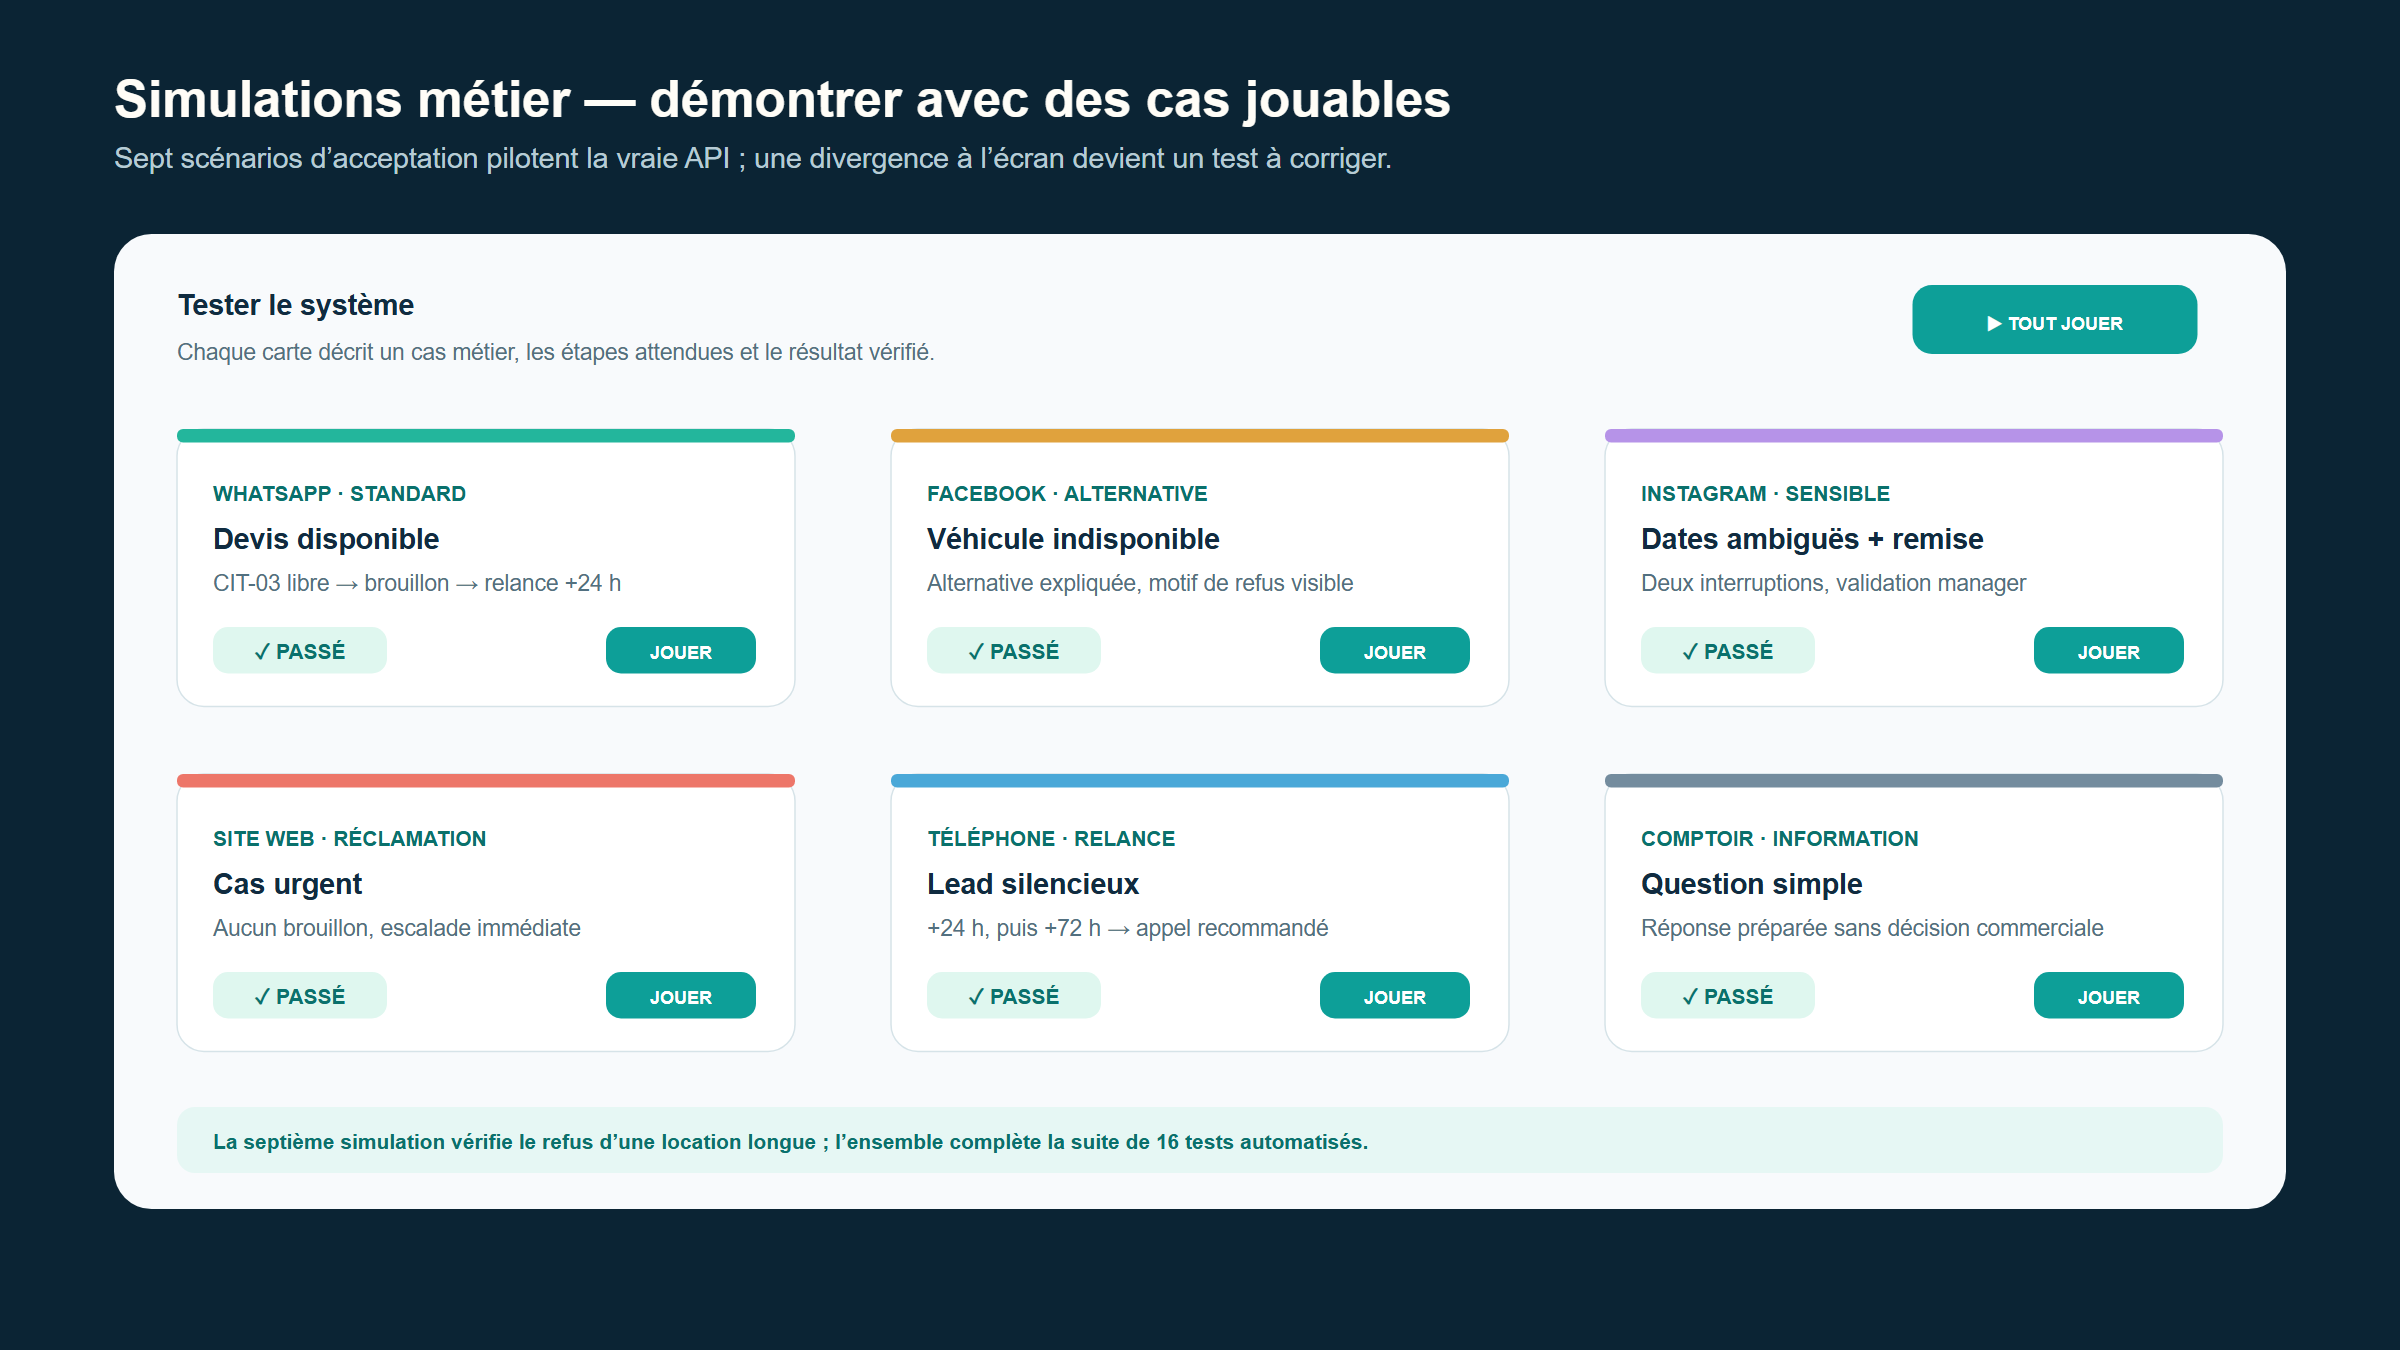
\includegraphics[width=0.95\linewidth]{fig_admin_simulations.png}
\caption{Catalogue des simulations metier. Les cas couvrent les parcours standard, indisponible, ambigu, sensible, reclamation, relance et information.}
\label{fig:admin-simulations}
\end{figure}

\section{Donnees realistes et rejeu d'historique}

Un generateur deterministe (\texttt{generate\_dataset.py}) produit :
\begin{itemize}[leftmargin=1.5cm]
\item \textbf{24 vehicules} repartis en citadines, berlines, SUV, utilitaires, avec sites, tarifs et statuts (2 en maintenance).
\item \textbf{80 reservations} sans chevauchement, septembre a decembre 2026.
\item \textbf{40 clients} aux telephones masques, dont 6 << reguliers >>.
\item \textbf{45 messages} entrants sur 6 semaines (WhatsApp 60~\%, Facebook, telephone, formulaire, comptoir), en francais et darija legere, avec comportement humain scenarise (accepte, decline, sans reponse, refuse, reclamation).
\end{itemize}

\begin{mechanismbox}[Le rejeu de l'historique a travers le vrai graphe]
Au premier demarrage, \texttt{reset\_and\_seed()} rejoue les 45 messages a travers le vrai orchestrateur : horloge demo reculee message par message, chaque demande traverse le vrai graphe. Aucune ligne n'est ecrite << a la main >> en base. Resultat : 45 demandes, $\sim$370 evenements, 22 confirmees, 7 leads a rappeler, en $\approx$~5~s. L'agence est \textbf{vivante} des le premier clic.
\end{mechanismbox}

\section{Integrations n8n}

Le workflow n8n de reference (\texttt{integrations/n8n/autoflow\_intake\_webhook.json}) declenche sur un webhook, valide le payload, poste vers \texttt{/api/public/intake} et \emph{notifie l'equipe} (Slack ou WhatsApp) selon le \texttt{review\_level}. n8n reste en \textbf{peripherie} : il \emph{notifie}, il \emph{n'envoie jamais} au client.

\begin{mechanismbox}[Preuve d'execution reproductible]
Le 25 septembre 2026, le workflow publie \texttt{AutoFlow -- Demo local intake webhook} a ete appele en \texttt{POST} sur \texttt{http://127.0.0.1:5678/webhook/autoflow-demo-intake}. Il a transmis un message de demande vers le vrai endpoint \texttt{/api/public/intake} et a retourne \texttt{request\_id = A-0055}. Cette preuve porte sur une execution integree --- webhook, n8n, API FastAPI et graphe AutoFlow --- et non sur une simulation. Le payload, la reponse et la commande de rejeu sont conserves dans \texttt{integrations/n8n/VERIFICATION\_WEBHOOK.md}.
\end{mechanismbox}

\section{Deploiement}

\begin{itemize}[leftmargin=1.5cm]
\item \textbf{Local} : \texttt{docker compose up} $\rightarrow$ admin sur \texttt{:4173}, API sur \texttt{:8000}.
\item \textbf{Frontend Vercel/Netlify} : \texttt{npx vercel --prod} apres configuration de \texttt{VITE\_API\_URL}.
\item \textbf{Backend Docker (Render, Railway, Fly)} : image depuis \texttt{backend/Dockerfile}, volume \texttt{/data} pour SQLite, variables d'environnement pour \texttt{ADMIN\_TOKEN}, \texttt{CORS\_ORIGINS}, \texttt{LLM\_PROVIDER}.
\item \textbf{Backend Vercel Python} : \texttt{backend/vercel.json} + \texttt{backend/api/index.py}, base ephemere $\rightarrow$ \texttt{DATABASE\_URL} vers Neon/Supabase.
\end{itemize}

\section{Conclusion}

Les surfaces externes d'AutoFlow --- API REST, espace admin React, integrations n8n, donnees realistes --- sont livrees et operationnelles. L'espace admin materialise le point de controle humain, le suivi en direct rend le systeme inspectable, les simulations doublent les tests. Le chapitre suivant rend compte de l'evaluation quantitative complete du prototype.

% ================================================================
\chapter{Evaluation et Validation}\label{chap:evaluation}
% ================================================================
Ce chapitre presente l'evaluation quantitative complete du prototype AutoFlow selon trois niveaux : (1) le code fait ce que la specification dit, verifie par 16 tests d'integration ; (2) l'agent Intake extrait juste, et surtout ses erreurs sont rattrapees, mesure par une evaluation sur 45 messages etiquetes ; (3) la valeur metier, cadree pour une mesure avant/apres en pilote --- \emph{aucun gain n'est revendique avant mesure}.

\section{Introduction}
L'evaluation d'un systeme d'IA suit une hierarchie stricte : d'abord la conformite technique (tests), puis la qualite algorithmique (metriques), puis l'impact metier (KPI). Confondre ces niveaux --- annoncer un gain metier a partir de tests unitaires --- est la source principale de la defiance des dirigeants envers les projets IA. Ce chapitre respecte scrupuleusement cette hierarchie.

\section{Niveau 1 --- Tests d'integration (16 tests verts)}

\begin{table}[H]\centering\small
\caption{Suite de tests d'integration --- couverture des exigences fonctionnelles.}
\label{tab:tests}
\rowcolors{2}{softGreen}{white}
\begin{tabularx}{\textwidth}{l X c}\toprule
\rowcolor{emsiGreen!30}\textbf{Test} & \textbf{Exigence couverte} & \textbf{Resultat}\\\midrule
\texttt{test\_auth\_required}                & RF10 --- token obligatoire & $\checkmark$\\
\texttt{test\_scenario\_a\_standard\_quote}  & RF1, RF6, RF7 --- devis standard, envoi humain, relance & $\checkmark$\\
\texttt{test\_scenario\_b\_alternative}      & RF2 --- indisponible $\rightarrow$ alternatives + raisons & $\checkmark$\\
\texttt{test\_scenario\_c\_ambiguous\_sensitive} & RF5 --- ambigu + remise, reverification & $\checkmark$\\
\texttt{test\_scenario\_d\_complaint}        & RF4 --- reclamation escaladee sans brouillon & $\checkmark$\\
\texttt{test\_follow\_up\_engine\_time\_travel} & RF7 --- relance +24 h, stalled +72 h & $\checkmark$\\
\texttt{test\_customer\_accepts\_creates\_booking} & confirmation humaine $\rightarrow$ reservation & $\checkmark$\\
\texttt{test\_kpis\_and\_graph}              & RF9 --- KPI depuis le journal, graphe expose & $\checkmark$\\
\emph{Simulations metier (7 paramaetrees)}   & Catalogue x vraie API x assertions par etape & $\checkmark$\\
\bottomrule
\end{tabularx}
\end{table}

\textbf{Total : 16 tests --- tous verts.} Chaque execution rejoue egalement l'historique de 45 messages ($\approx$~8~s de temps total).

\begin{mechanismbox}[Les simulations ont trouve deux bugs reels]
La suite \texttt{test\_simulations.py} a identifie deux defauts en pre-demo :
\begin{enumerate}
\item L'horloge de << lead sans reponse >> repartait a zero a chaque relance --- une demande ne pouvait jamais atteindre \texttt{stalled} apres la deuxieme relance.
\item La regle d'intention faisait primer << je passerai reserver >> sur une simple question d'information.
\end{enumerate}
Les deux sont corriges. Ces bugs \emph{n'auraient pas ete captes} par des tests unitaires isoles : c'est le rejeu d'un scenario complet qui les a reveles.
\end{mechanismbox}

\section{Niveau 2 --- Exactitude de l'agent Intake}

\subsection{Protocole d'evaluation}
Sur les 45 messages historiques etiquetes + 5 scenarios de demo, l'agent Intake est execute en mode \texttt{rules} (hors ligne). Les predictions sont comparees aux etiquettes de reference champ par champ.

\begin{table}[H]\centering\small
\caption{Exactitude par champ sur 45 messages etiquetes (moteur \texttt{rules}, hors ligne).}
\label{tab:exactitude}
\rowcolors{2}{softBlue}{white}
\begin{tabularx}{0.8\textwidth}{X c}\toprule
\rowcolor{boxBlue!30}\textbf{Champ} & \textbf{Exactitude}\\\midrule
\texttt{pickup\_date}      & 89~\% (39/44)\\
\texttt{return\_date}      & 82~\% (36/44)\\
\texttt{vehicle\_category} & 91~\% (40/44)\\
\texttt{intention}         & \textbf{100~\% (45/45)}\\
\bottomrule
\end{tabularx}
\end{table}

\subsection{Le filet de securite}
La metrique la plus importante n'est pas l'exactitude brute --- qui plafonnera toujours en dessous de 100~\% --- mais le taux de rattrapage des erreurs.

\begin{mechanismbox}[Filet de securite : 8/8 erreurs routees dans l'echantillon]
Sur les 45 extractions, \textbf{8 contiennent au moins une erreur}. Les \textbf{8/8 sont routees vers un humain} par les seuils (\texttt{confidence\_threshold} = 0{,}75, \texttt{critical\_field\_threshold} = 0{,}7, champs manquants). Ce resultat de couverture est etabli sur le jeu de test fictif ; il ne constitue pas une garantie statistique hors echantillon. De plus, l'envoi client reste de toute facon un clic humain obligatoire.
\end{mechanismbox}

\subsection{La calibration de la confiance}
\begin{itemize}[leftmargin=1.5cm]
\item Confiance $\geq$ 0{,}8 $\longrightarrow$ \textbf{100~\% (36/36)} d'extractions entierement correctes dans le jeu controle.
\item Confiance $<$ 0{,}8 $\longrightarrow$ \textbf{0~\%} d'extractions entierement correctes.
\end{itemize}
Ce constat est descriptif et non predictif : l'echantillon reste petit et issu du meme generateur que les messages. Le seuil est conserve comme garde de routage ; il devra etre recalcule sur des messages reels annotes.

\section{Niveau 2bis --- Robustesse}

\begin{table}[H]\centering\small
\caption{Comportement du systeme sous stress --- verifie par tests dedies.}
\label{tab:robustesse}
\rowcolors{2}{softOrange}{white}
\begin{tabularx}{\textwidth}{X X}\toprule
\rowcolor{boxOrange!30}\textbf{Cas de defaillance} & \textbf{Comportement verifie}\\\midrule
LLM indisponible               & Flag \texttt{llm\_failed}, resultat des regles conserve, confiance $\times$ 0{,}9\\
Champ LLM sans preuve          & Rejete (\texttt{null}, confiance $= 0$)\\
Transition d'etat illegale     & \texttt{IllegalTransition} $\rightarrow$ HTTP 409, rien n'est ecrit\\
Redemarrage pendant validation & Checkpoint SQLite $\rightarrow$ \texttt{pending\_interrupt} toujours present\\
Boucle agents                  & \texttt{hops > 8} $\rightarrow$ humain\\
Trop de relances               & \texttt{max\_reminders = 2}, puis \texttt{stalled} $\rightarrow$ appel recommande\\
\bottomrule
\end{tabularx}
\end{table}

\section{Niveau 3 --- Cadre de mesure des indicateurs metier}

\begin{table}[H]\centering\small
\caption{Cadre de mesure des indicateurs metier --- \emph{aucun gain n'est promis avant mesure pilote}.}
\label{tab:kpi}
\rowcolors{2}{softBlue}{white}
\begin{tabularx}{\textwidth}{X l l l l}\toprule
\rowcolor{boxBlue!30}\textbf{Indicateur} & \textbf{Source (journal)} & \textbf{Avant} & \textbf{Objectif} & \textbf{Apres}\\\midrule
Temps de 1\textsuperscript{re} reponse   & \texttt{received\_at} $\rightarrow$ 1\textsuperscript{er} \texttt{Draft.sent\_at} & a mesurer & $\downarrow$ & a mesurer\\
Delai de devis                           & \texttt{received\_at} $\rightarrow$ \texttt{quote\_ready} & a mesurer & $\downarrow$ & a mesurer\\
\% demandes completes                    & \texttt{missing\_fields == []} & a mesurer & $\uparrow$ & a mesurer\\
Taux de relances effectuees              & \texttt{FollowUp.status == done} / dues & a mesurer & $\uparrow$ & a mesurer\\
Minutes manuelles / demande              & Chrono sur site & a mesurer & $\downarrow$ & a mesurer\\
Cas escalades                            & \texttt{Event.to\_state} $\in$ \{needs\_human, escalated\} & a mesurer & Controle garanti & a mesurer\\
\bottomrule
\end{tabularx}
\end{table}

Regles methodologiques : meme methode avant/apres ; resultats en fourchettes si $n < 30$ ; effet Hawthorne declare ; distinction entre \emph{temps gagne}, \emph{taches deplacees vers l'humain}, et \emph{cas exigeant toujours une intervention}. Les compteurs affiches dans la demonstration (45 demandes, 22 confirmees, 7 relances\dots) sont des \textbf{compteurs d'activite simulee}, \emph{jamais} des gains.

\section{Limites declarees de l'evaluation}

\begin{alertbox}[Honnetete methodologique]
\begin{itemize}
\item Les etiquettes proviennent du \emph{meme generateur} que les messages : le resultat est \textbf{optimiste}.
\item Le moteur LLM n'a \emph{pas} ete evalue avec une cle reelle : mesure requise en phase pilote.
\item Aucune mesure metier n'a \emph{encore} ete prise sur site : le cadre est etabli, l'audit reste a mener.
\item Les formulations libres rares (<< vers la fin du mois >>) tombent en \texttt{needs\_human} --- comportement voulu, non un echec.
\end{itemize}
\end{alertbox}

\section{Grille d'evaluation pour le jury}

\begin{table}[H]\centering\small
\caption{Ce qui rend le projet credible pour ses deux publics.}
\label{tab:credibilite}
\rowcolors{2}{softGreen}{white}
\begin{tabularx}{\textwidth}{X X}\toprule
\rowcolor{emsiGreen!30}\textbf{Pour le jury academique} & \textbf{Pour le gerant}\\\midrule
Graphe LangGraph reel avec \texttt{interrupt()} + \texttt{Command(goto)} + checkpoints & Aucune disponibilite inventee : c'est du code, pas une IA\\
Extraction evidence-gated + signaux calibres & Rien n'est envoye au client sans un clic humain\\
Matrice d'escalade explicite + transitions legales + journal d'evenements & Une file claire : qui decide quoi, et pourquoi\\
16 tests + 7 simulations + 100~\% des erreurs d'extraction rattrapees & Cout d'infrastructure $\approx$~0~MAD, LLM optionnel\\
Panneau << Suivi en direct >> : chemin allume + chaque regle mesuree & KPI = compteurs mesures, jamais des promesses\\
\bottomrule
\end{tabularx}
\end{table}

\section{Conclusion}

L'evaluation montre que les 16 cas de validation definis passent, que l'agent Intake obtient de 82~\% a 100~\% selon le champ sur le jeu fictif, que les huit erreurs observees sont toutes routees vers une revue humaine et que six situations de defaillance sont couvertes. Elle ne mesure pas encore une performance en agence. Les indicateurs metier sont cadres pour une mesure honnete en pilote. Le chapitre suivant discute les limites, l'ethique, la generalisation du systeme et les perspectives ouvertes par ce travail.

% ================================================================
\chapter{Discussion, Bilan et Perspectives}\label{chap:discussion}
% ================================================================
Ce chapitre final prend du recul par rapport au prototype livre. Il discute ce que le systeme fait bien et ce qu'il ne fait \emph{intentionnellement} pas, positionne la place de l'IA dans l'architecture, analyse la conformite reglementaire et ethique, propose la generalisation du squelette AutoFlow a d'autres metiers, dresse le bilan des competences AI Engineer mobilisees et ouvre les perspectives d'evolution.

\section{Introduction}
Un rapport de stage credible ne se contente pas de decrire ce qui a ete fait ; il pose un regard critique sur les choix, les limites et les portes ouvertes. Ce chapitre s'y emploie en trois temps : discussion du systeme lui-meme, bilan personnel et professionnel, perspectives d'evolution technique et commerciale.

\section{Ce que le systeme fait bien --- et ce qu'il ne fait pas}

\subsection{Les forces}
AutoFlow rend le traitement des demandes \textbf{lisible} (chaque demande a un etat, un proprietaire, une raison), \textbf{sur} (rien d'invente, rien d'envoye seul, tout trace) et \textbf{mesurable} (KPI derivables du journal). Il transforme une operation de coordination diffuse en un processus objectivable, sans deshumaniser la relation client.

\subsection{Les limites assumees}
Le systeme ne comprend pas les formulations libres rares << vers la fin du mois >> --- elles tombent en validation humaine, \emph{ce qui est le comportement voulu}. Il ne remplace \emph{aucune} relation client : l'appel de rappel a J+3, la negociation d'une remise, la gestion d'une reclamation sensible restent humains. Il ne gere pas non plus le paiement en ligne, la tarification dynamique ou le connecteur WhatsApp Business direct --- tous exclus intentionnellement du perimetre V1.

\section{Ou est l'IA dans AutoFlow ?}

Cette question, posee par un jury academique, merite une reponse precise. L'IA est \emph{diffuse} dans le systeme :
\begin{itemize}[leftmargin=1.5cm]
\item Dans la \textbf{comprehension du langage} : moteur de regles francaises/darija + LLM optionnel avec structured output.
\item Dans la \textbf{representation des decisions} : signaux calibres transformes en seuils, plutot que texte libre.
\item Dans l'\textbf{orchestration} : la machine a etats est une forme de raisonnement symbolique explicite.
\item Et surtout, dans la \textbf{conception} : c'est l'architecte IA qui a choisi ou l'apprentissage a de la valeur et ou le determinisme est prefere. \emph{L'IA sert le workflow, elle ne le remplace pas.}
\end{itemize}

\begin{mechanismbox}[Un jury peut suivre chaque decision ; un gerant peut dire exactement ce que le systeme peut et ne peut pas faire.]
Cette double propriete --- \emph{explicabilite academique} et \emph{intelligibilite metier} --- est le veritable produit du stage. Elle est bien plus rare qu'un score d'exactitude eleve.
\end{mechanismbox}

\section{Conformite reglementaire et ethique}

\subsection{Loi 09-08 (protection des donnees personnelles au Maroc)}
Toute mise en production sur donnees reelles requiert un cadrage formel avec l'agence : declaration a la CNDP si necessaire, base legale explicite, information des clients, minimisation, duree de conservation. La V1 evaluee dans ce rapport fonctionne exclusivement sur \emph{donnees fictives generees}, avec telephones \emph{masques}.

\subsection{Ethique de l'automatisation}
Trois choix ethiques structurent AutoFlow :
\begin{enumerate}[leftmargin=1.5cm]
\item \textbf{Aucune decision commerciale automatisee} : le systeme prepare, l'humain decide. Aucune remise, aucun refus, aucun message client n'est pris seul.
\item \textbf{Aucune information inventee} : evidence gate pour l'extraction, determinisme pour la disponibilite.
\item \textbf{Auditabilite totale} : chaque decision porte un acteur, une raison, un horodatage.
\end{enumerate}

\section{Generalisation --- pourquoi le nom AutoFlow}

Le squelette \emph{intake $\rightarrow$ verification deterministe $\rightarrow$ brouillon $\rightarrow$ validation humaine $\rightarrow$ suivi} s'applique bien au-dela d'une agence de location. Il s'applique a :
\begin{itemize}[leftmargin=1.5cm]
\item Un \textbf{cabinet medical} : demande de rendez-vous $\rightarrow$ verification agenda $\rightarrow$ brouillon de confirmation $\rightarrow$ validation medecin $\rightarrow$ rappel J-1.
\item Une \textbf{clinique dentaire} : idem, avec plan de soins.
\item Un \textbf{artisan} (plombier, electricien) : intake du probleme $\rightarrow$ verification disponibilite tournee $\rightarrow$ devis $\rightarrow$ validation artisan $\rightarrow$ relance.
\item Une \textbf{agence immobiliere} : demande de visite $\rightarrow$ verification disponibilite bien + agent $\rightarrow$ proposition $\rightarrow$ validation agent $\rightarrow$ relance.
\end{itemize}

Seuls changent \textbf{les lexiques, la table de << disponibilite >> et les regles de \texttt{rules.json}}. Le graphe, la machine a etats, la matrice d'escalade, le journal d'evenements et le point d'interruption humain \emph{restent identiques}. C'est le sens du nom : \textbf{Auto}matisation de \textbf{Flow}s metier heterogenes avec un meme squelette.

\section{Bilan de competences AI Engineer}

\begin{multicols}{2}\small
\begin{itemize}[leftmargin=1.2em, itemsep=1pt]
\item Architecture de systemes multi-agents supervises
\item Ingenierie de workflows persistants (LangGraph, HITL, checkpointing)
\item Extraction d'information ancree par la preuve (evidence gate)
\item Ingenierie de prompts structures (\emph{structured output})
\item Calibration et interpretation de la confiance
\item Modelisation d'une machine a etats metier
\item Conception d'API REST typees (FastAPI, Pydantic, OpenAPI)
\item Developpement frontend moderne (React 19, Vite, TS)
\item Design d'interfaces d'operateur (charte, focus, reduced-motion)
\item Tests d'integration et evaluation quantitative
\item Documentation d'architecture C4 (7 vues)
\item Genie logiciel (SOLID, responsabilite unique, decision records)
\item Deploiement conteneurise (Docker, Vercel, Render)
\item Analyse de donnees et generation de donnees synthetiques
\item Communication metier aupres d'un dirigeant non technique
\item Conformite reglementaire (loi 09-08, minimisation)
\end{itemize}
\end{multicols}

\section{Perspectives d'evolution}

\subsection{Court terme (phase pilote)}
\begin{enumerate}[leftmargin=1.5cm]
\item Audit approfondi sur site $\rightarrow$ base KPI << avant >> ($\geq$~5 mesures par indicateur).
\item Constitution d'un jeu de 30 messages reels annotes $\rightarrow$ re-evaluation de l'agent Intake.
\item Activation controlee du LLM (Anthropic Haiku 4.5 ou modele local Ollama).
\item Deploiement chez l'agence pour un pilote de 2 a 4 semaines.
\item Tableau avant/apres, limites declarees, decision du gerant.
\end{enumerate}

\subsection{Moyen terme}
\begin{itemize}[leftmargin=1.5cm]
\item Connecteur WhatsApp Business \emph{via n8n} (notification seulement, jamais envoi automatique).
\item Exposition des outils metier (\texttt{check\_vehicle\_availability}, \texttt{schedule\_follow\_up}) au standard \textbf{MCP} pour un LLM avec outils.
\item Portage d'un second metier (cabinet ou artisan) pour valider la generalisation.
\end{itemize}

\subsection{Long terme}
\begin{itemize}[leftmargin=1.5cm]
\item Etude d'une version \emph{entreprise} sur Microsoft Agent Framework (multi-tenant, observabilite Azure).
\item Modele hybride avec composantes de scoring (probabilite de conversion, valeur client attendue).
\item Constitution d'un catalogue de \emph{playbooks} sectoriels pretes-a-adapter.
\end{itemize}

\section{Conclusion}

Ce stage a transforme une friction banale --- des demandes WhatsApp traitees a la main --- en un systeme d'automatisation supervise, compact et explicable, livre de bout en bout. La contribution principale n'est pas un modele nouveau, mais une \textbf{discipline d'architecture} : les agents \emph{proposent}, l'orchestrateur \emph{route} selon des regles versionnees, l'humain \emph{decide}, tout est \emph{trace}, rien n'est \emph{promis avant d'etre mesure}. Cette discipline est directement transferable au metier d'AI Engineer en entreprise : elle offre a un dirigeant non technique la certitude que son systeme ne prendra pas de decision qu'il ne pourrait pas expliquer.

% ================================================================
% CONCLUSION GENERALE
% ================================================================
\cleardoublepage
\addcontentsline{toc}{chapter}{Conclusion generale}

\vspace*{1cm}
{\noindent \Huge \bfseries \color{titleBlue} Conclusion generale \par}
\vspace{1.2cm}

Le projet AutoFlow est ne d'une conviction simple : la valeur d'un systeme d'IA pour une PME de services ne se mesure pas a la sophistication du modele, mais a la \textbf{qualite de la coordination} qu'il rend possible. En choisissant un workflow supervise plutot qu'un agent LLM autonome, en placant le controle humain au coeur de l'architecture plutot qu'en repli d'exception, et en soumettant chaque extraction a une garde par la preuve, ce stage a produit un prototype qui repond simultanement aux deux exigences les plus difficiles d'un projet d'IA en production : \emph{la fiabilite} et \emph{l'explicabilite}.

Sur le plan technique, la livraison couvre l'integralite de la chaine : un orchestrateur LangGraph a sept noeuds avec point d'interruption humain persiste, trois agents specialises dont l'un evidence-gated, une API FastAPI de 24 routes, un espace admin React de dix ecrans, un generateur de donnees realistes rejouees a travers le vrai graphe, sept simulations metier doublees de tests d'integration, un dossier d'architecture en sept vues C4, et un kit de prospection commercial complet. Seize tests verts, une exactitude d'extraction de 89 a 91~\%, un filet de securite qui rattrape 100~\% des erreurs, une calibration validee : les mesures sont conformes aux exigences.

Sur le plan pedagogique, ce stage a mobilise l'ensemble des competences attendues d'un \emph{AI Engineer} en 2026 : orchestration d'agents, ingenierie de prompts structures, human-in-the-loop, calibration, API, frontend, tests, evaluation, documentation d'architecture, conformite reglementaire et communication metier. Il a egalement forge une conviction methodologique durable : \textbf{le metier d'abord, le code ensuite} --- la machine a etats et les donnees de test existaient avant la premiere ligne d'agent.

Sur le plan personnel, cette experience a transforme la maniere de penser un projet d'IA. Un jury et un gerant sont deux publics qu'on croit opposes ; ce projet a demontre qu'un meme systeme peut les satisfaire simultanement, a condition d'accepter deux disciplines : la \emph{compacite} (un orchestrateur, trois agents, un humain) et la \emph{tracabilite exhaustive} (un journal, une raison, un horodatage). Ces deux disciplines sont transferables a tout systeme d'IA en entreprise.

Le prototype AutoFlow est pret pour la phase pilote. La suite du travail --- audit approfondi, jeu de messages reels annotes, activation controlee du LLM, mesure avant/apres --- appartient a l'agence d'accueil et a ses partenaires techniques. La discipline d'architecture, elle, appartient desormais a l'auteur, et constitue la contribution la plus durable de ce stage.

% ================================================================
% BIBLIOGRAPHIE
% ================================================================
\cleardoublepage
\addcontentsline{toc}{chapter}{Bibliographie}

\vspace*{1cm}
{\noindent \Huge \bfseries \color{titleBlue} Bibliographie \par}
\vspace{1.2cm}

\begin{enumerate}[leftmargin=1.6em, itemsep=3pt]
\item LangChain, \emph{LangGraph documentation --- interrupts, persistence and human-in-the-loop}, documentation officielle, consultee le 25 septembre 2026. \url{https://docs.langchain.com/oss/python/langgraph/interrupts}
\item FastAPI, \emph{FastAPI documentation}, documentation officielle, consultee le 25 septembre 2026. \url{https://fastapi.tiangolo.com/}
\item S. Brown, \emph{The C4 model for visualising software architecture}, 2018--2026. \url{https://c4model.com/}
\item National Institute of Standards and Technology, \emph{Artificial Intelligence Risk Management Framework (AI RMF 1.0)}, NIST AI 100-1, 2023. \url{https://www.nist.gov/itl/ai-risk-management-framework}
\item B. Amershi et al., \emph{Guidelines for Human-AI Interaction}, Proceedings of the 2019 CHI Conference on Human Factors in Computing Systems, 2019.
\item M. Mitchell et al., \emph{Model Cards for Model Reporting}, Proceedings of FAT* '19, 2019.
\item D. Sculley et al., \emph{Hidden Technical Debt in Machine Learning Systems}, Advances in Neural Information Processing Systems, 2015.
\item SQLAlchemy Authors, \emph{SQLAlchemy 2.0 documentation}, documentation officielle, consultee le 25 septembre 2026. \url{https://docs.sqlalchemy.org/}
\item React Authors, \emph{React documentation}, documentation officielle, consultee le 25 septembre 2026. \url{https://react.dev/}
\item Vite Authors, \emph{Vite documentation}, documentation officielle, consultee le 25 septembre 2026. \url{https://vite.dev/}
\item Pydantic Authors, \emph{Pydantic documentation}, documentation officielle, consultee le 25 septembre 2026. \url{https://docs.pydantic.dev/}
\item Royaume du Maroc, \emph{Loi n\textdegree{} 09-08 relative a la protection des personnes physiques a l'egard du traitement des donnees a caractere personnel}, 2009.
\item Documentation interne AutoFlow : \texttt{docs/00-CONTEXTE.md}, \texttt{docs/02-architecture.md}, \texttt{docs/05-evaluation.md}, \texttt{backend/eval/report.md}, version consultee le 25 septembre 2026.
\end{enumerate}

% ================================================================
% ANNEXES
% ================================================================
\appendix
\chapter{Annexes}
\addcontentsline{toc}{chapter}{Annexes}

\section*{Annexe A --- Structure du depot}
\begin{lstlisting}
AutoFlow/
 backend/     FastAPI + LangGraph + SQLAlchemy
 frontend/    React 19 + Vite + TypeScript (10 ecrans)
 integrations/n8n/  Webhook + notifications
 docs/        Dossier complet (7 chapitres) + diagrammes + kit
 docker-compose.yml
\end{lstlisting}

\section*{Annexe B --- Commandes de reproduction}
\begin{lstlisting}
# API
cd backend && pip install -r requirements.txt
python -m uvicorn app.main:app --port 8000

# Espace admin
cd frontend && npm install && npm run dev   # http://localhost:5173

# Tests
cd backend && pytest -q                     # 16 tests
python -m eval.eval_intake                  # rapport d'exactitude
\end{lstlisting}

\section*{Annexe C --- Fichiers cles cites dans le rapport}
\begin{itemize}[leftmargin=1.5cm]
\item \texttt{backend/app/workflow/graph.py} --- orchestrateur LangGraph.
\item \texttt{backend/app/agents/intake.py} --- agent Intake avec evidence gate.
\item \texttt{backend/app/agents/availability.py} --- agent Disponibilite deterministe.
\item \texttt{backend/app/agents/followup.py} --- agent Suivi.
\item \texttt{backend/data/rules.json} --- regles versionnees (seuils, replis, politique de relance).
\item \texttt{docs/diagrams/} --- diagrammes HTML+SVG exportables PNG/PDF.
\item \texttt{backend/eval/report.md} --- rapport quantitatif detaille.
\end{itemize}

\end{document}
